\documentclass{article}

\usepackage[numbers,sort &compress]{natbib}
\usepackage[english]{babel}
\usepackage[utf8]{inputenc}
\usepackage{amsmath,amssymb}
\usepackage{parskip}
\usepackage{graphicx}
\usepackage[utf8]{inputenc}
\usepackage[english]{babel}
\usepackage{rotating}
 
\usepackage[nottoc]{tocbibind}

% Margins
\usepackage[top=2.5cm, left=3cm, right=3cm, bottom=4.0cm]{geometry}
% Colour table cells
\usepackage[table]{xcolor}

% Get larger line spacing in table
\newcommand{\tablespace}{\\[1.25mm]}
\newcommand\Tstrut{\rule{0pt}{2.6ex}}         % = `top' strut
\newcommand\tstrut{\rule{0pt}{2.0ex}}         % = `top' strut
\newcommand\Bstrut{\rule[-0.9ex]{0pt}{0pt}}   % = `bottom' strut

%%%%%%%%%%%%%%%%%
%     Title     %
%%%%%%%%%%%%%%%%%
\title{Efficient Reinforcement Learning with Initialized Policy}
\author{Author: Zihan Ding\\Supervisor: Dr. Edward Johns\\Department of Computing\\Imperial College London}

\date{\today}

\begin{document}
\maketitle
\newpage
\tableofcontents
%%%%%%%%%%%%%%%%%
%   Problem 1   %
%%%%%%%%%%%%%%%%%

\newpage
\begin{abstract}
How can we improve the efficiency of reinforcement learning algorithms, and make it more feasible for real-world applications like robotic control? A promising way is to initialize the policy with pre-trained weights, and learning the initial weights can be regarded as a `meta-learning' process for improving performances in reinforcement learning on tasks, i.e. learning how to initialize a policy for a specific task. The initialization policy is useful as it contains additional information, which can be obtained from different sources, like leveraging expert demonstrations, or meta-learned policy across tasks without demonstrations. These two main approaches are investigated thoroughly with experiments and comparisons in this paper, with tasks on a simulated environment called \textit{Reacher} as a simplified robotic arm. The experimental algorithms are based on model-free reinforcement learning, including deep deterministic policy gradient (DDPG), proximal policy optimization (PPO), etc, for off-policy and on-policy algorithms respectively. For the first approach of leveraging expert demonstrations, methods including behaviour cloning, residual policy learning and directly feeding demonstrations into memory buffer are implemented and analyzed in the experimental sections, and results together with conclusions are given. Other methods including reward shaping, optimistic initialization are also introduced. For the second approach of meta-learning across tasks without demonstrations, different variants of modal-agnostic meta-learning including first-order modal-agnostic meta-learning and Reptile methods are compared with learning from scratch in experiments. Other methods like universal successor representation in the category without demonstrations are also introduced. Using different methods mentioned above with or without demonstrations, we can practically improve the efficiency of reinforcement learning process to some different extents. Details for comparison of different methods are shown in the experimental sections.
\end{abstract}

\newpage

\section{Introduction}
Reinforcement learning (RL), especially deep reinforcement learning (DRL), always suffers from the problem of poor learning efficiency for large-scale high-dimensional applications like robot control in reality. Existing RL algorithms usually need a large number of samples from interactions with the environment to learn an effective policy. 

In order to improve the efficiency of RL, additional information needs to be provided for the learning agent. There are main two sources of information could be incorporated into the reinforcement learning process in general: (1). demonstrations from expert; (2). knowledge from similar tasks in a task domain. 

The first approach is usually feasible for a single specific task. With demonstrations from an expert, the learning agent is able to perform an imitation learning and therefore learn much faster than learning from scratch. But imitation learning cannot provide an optimal policy for general cases, and it is always restricted by the amount of demonstration data and the performance level of the expert. Alternatively, we can take the imitation learning process with demonstrations as an initialization for a subsequent RL process, to learn an optimal policy on a task finally.

The second approach is for RL to learn a policy for a new task quickly, based on the transferred knowledge from other tasks within in the same task domain, which can also be called meta-learning. No demonstrations are needed for this approach. We also take the policy trained across tasks as an initialization for a new task.

Initialization is a key point when applying neural networks \cite{glorot2010understanding}, and proper initialization will improve the learning performance greatly in DRL. Knowledge and underlying principles are represented as values of parameters in a neural network, if trained properly. How to initialize a RL policy remains a challenge for efficient RL. We did a survey about present methods for alleviating the efficiency problem of RL, focusing on the initialization settings of policy with above two approaches. For the first approach with demonstrations, we investigate the properties of present methods thoroughly, including policy replacement or called behavioural cloning, residual policy learning, directly feeding demonstrations into the memory buffer, and show the comparison of these methods under different circumstances. Some conclusions are given based on the experiments. Moreover, we introduce other methods including normalized actor-critic, reward shaping, optimistic initialization, etc. For the second approach without demonstrations, we investigate present meta-learning algorithms including modal-agnostic meta-learning and different variants of it. Experiments are conducted to show the improvement when applying meta-learning as an initialization for RL. We further introduce other initialization methods for RL without demonstrations like universal successor representation, etc.

There are other approaches for improving training efficiency for RL including model-based methods like Guided Policy Search \cite{levine2013guided}, or model-free methods with model-based acceleration like Normalized Advantage Functions (NAF) \cite{gu2016continuous}. But we will mainly focus on model-free methods for RL in this paper. And the RL algorithms we used in experiments are all model-free based.

The paper is developed as follows: the first chapter is the introduction; the second chapter is descriptions of basic concepts in RL and some of the present RL algorithms; the third chapter is description about the {Reacher} environment we applied in simulated experiments; the fourth chapter is initialization of RL with demonstrations, including illustrations of present methods and experimental comparisons; the fifth chapter is initialization of RL without demonstrations, including illustrations of meta-learning as initialization and experimental results, and some other methods are also described in this chapter.


\section{Reinforcement Learning}
\subsection{Background}\label{Background}
Reinforcement learning (RL) \cite{sutton2018reinforcement}\cite{arulkumaran2017brief} is a topic aside from supervised learning and unsupervised learning, with strong correlations in applications like robotics control. Reinforcement learning can be illustrated typically using the Fig. \ref{fig:rl0}\footnote{Cited from https://media.nips.cc/Conferences/2016/Slides/6198-Slides.pdf}, which demonstrates the interaction learning process of RL agent with an environment. 

The overall goal of RL is to maximize the expected total reward, which can be formalized in the following process. We first consider a series of states $(s_0, s_1, ..., s_t, ...)$ describing the environment changing through the interaction process of the agent and the environment, and we suppose that for each state transformation $(s_t, s_{t+1})$ there is a corresponding action $a_t$ of the agent which leads to the transformation, no matter deterministically or non-deterministically (stochastically). Therefore the state series are extended as $(s_0, a_0, s_1, a_1, ..., s_t, a_t, ...)$. And we also suppose that there is always a reward $r_t$ corresponding with each state $s_t$. Then we have $(s_0, a_0, r_0, s_1, a_1, r_1, ..., s_t, a_t, r_t,...)$. With an absorbing state, the sequence will be finite; and it will be infinite without an absorbing state. We can hence formalize the total reward as $R=\sum_{t=0}^{\infty or T}r_t$ for infinite/finite process. And the probability of the above total reward is the probability of the sequence of state transformation: $P(s_0, a_0, r_0, s_1, a_1, r_1, ..., s_t, a_t, r_t,...)$. Therefore we want to maximize the expected total reward with the following relationship:
\begin{equation}
    \max\mathbb{E}_{P(s_0, a_0, r_0, s_1, a_1, r_1, ..., s_t, a_t, r_t,...)}[\sum_{t=0}^{\infty}r_t]
\end{equation}
and the expectation is taken as the process of interaction is always stochastic. The maximization is taken over the parameterized policy $\pi_\theta$ which determines the sequential transformation probability. Now we try to specify and simplify the above equation.

\textbf{Assumption 1.} Markov process: we take the state transformation as a markov process, and we have $P(s_{t+1}|s_t, s_{t-1},...,s_0)=P(s_{t+1}|s_t)$, and therefore: \begin{equation}
    P(s_0, a_0, r_0, s_1, a_1, r_1, ..., s_t, a_t, r_t,...) = P(s_0, r_0)\Pi_{t=0}^\infty (P((s_{t+1}, r_{t+1})|(s_t,a_t,r_t))P(a_{t}|s_{t}))
\end{equation}

\textbf{Assumption 2.} Deterministic transformation process: we assume the transformation matrix described by $P((s_{t+1}, r_{t+1})|(s_t,a_t,r_t)$ is deterministic and therefore the probability equals to 1. So we have,
\begin{equation}
    P(s_0, a_0, r_0, s_1, a_1, r_1, ..., s_t, a_t, r_t,...) = P(s_0, r_0)\Pi_{t=0}^\infty P(a_{t}|s_{t})
\end{equation}
where the $P(s_0, r_0)$ is probability of different starting state.

We usually use logarithm in practice (the logarithmic derivative trick) and denote $P(a_{t}|s_{t})$ as the parameterized policy $\pi_\theta$ we want to learn. Therefore we have the gradients of optimization goal (the reward term has no relationship with policy parameters $\theta$ and neglect the constant term like probability of initial state):
\begin{equation}
\begin{aligned}
\label{equ:policy_gradient}
    g&=\nabla_\theta \mathbb{E}[\sum_{t=0}^\infty \Phi_t \log \pi_\theta(a_t|s_t)]\\
    &=\mathbb{E}[\sum_{t=0}^\infty \Phi_t \nabla_\theta \log \pi_\theta(a_t|s_t)]
\end{aligned}
\end{equation}
where $\Phi_t$ is the term of reward/value/advantage describing how good current state is with respect to direct rewards from the environment. It have several different expressions as shown in \cite{schulman2015high}. 
Eq. (\ref{equ:policy_gradient}) is called the policy gradient.

Deep reinforcement learning (DRL) \cite{arulkumaran2017deep} is gradient-based RL algorithms with deep neural networks as approximators, which composes the majority of present RL methods. RL can also be addressed with gradient-free methods like evolutionary methods \cite{koutnik2013evolving}.

\begin{figure}[htbp]
	\centering
	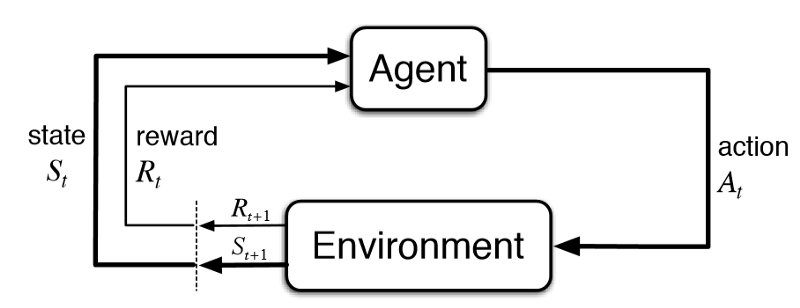
\includegraphics[scale=0.4]{img/rl.png}
	\caption{A basic architecture of reinforcement learning.}
	\label{fig:rl0}
\end{figure}
\subsection{Discrete and Continuous Action Space}
There are two types of action space for general RL problem: the continuous one and the discrete one. RL algorithms like Q-learning, Deep Q-Network can only work for discrete action space without further modifications. And algorithms like REINFORCE, Actor-Critic, DDPG, TRPO, PPO, etc can work for continuous action space, and sometimes work for discrete action space with a few proper modifications.

The discrete and continuous action space can transform into each other to some extent. A continuous action space problem can be sometimes be solved through discretization of the potential action values and applying a discrete RL algorithm; a discrete action space problem can also be handled with continuous RL algorithms if the output action values are discretized properly. However, there is always a cost for the transformation in different action spaces. If a discrete RL algorithm has to be used for a task with a continuous action space, the possible number of the discretized action values could be large to have a similar control effect as a continuous RL algorithm, which would be hard to learn in practice for the RL agent.

\subsection{Deterministic and Stochastic Policy}
There are two types of action choice in a RL policy, the deterministic one and the stochastic one. The deterministic policy like DDPG uses the pathwise derivative estimators (differentiate through the action value) while the stochastic action policy like REINFORCE and so on applies the score function estimator using the log derivative trick (differentiate through the log probability of action choice, sometimes also through the action value).  The deterministic policy in DRL is that the action values are directly determined by the outputs of neural networks. Algorithms including DQN and DDPG are deterministic policy. The stochastic policy is that the action values are sampled from a distribution parametrized by the direct outputs of neural networks, therefore the action values themselves are not directly determined by the outputs of neural networks. Algorithms including REINFORCE, Actor-Critic, TRPO and PPO are stochastic policy.
\subsection{Reinforcement Learning Algorithms}
Fig. \ref{fig:rl}\footnote{Cited from Twitter} shows a development of RL algorithms for recent years. We introduce some model-free RL algorithms as follows, including the REINFORCE, Actor-Critic, Q-learning, deep Q-network, deep deterministic policy gradient, trust region policy optimization, proximal policy optimization, etc.
\begin{figure}[htbp]
	\centering
	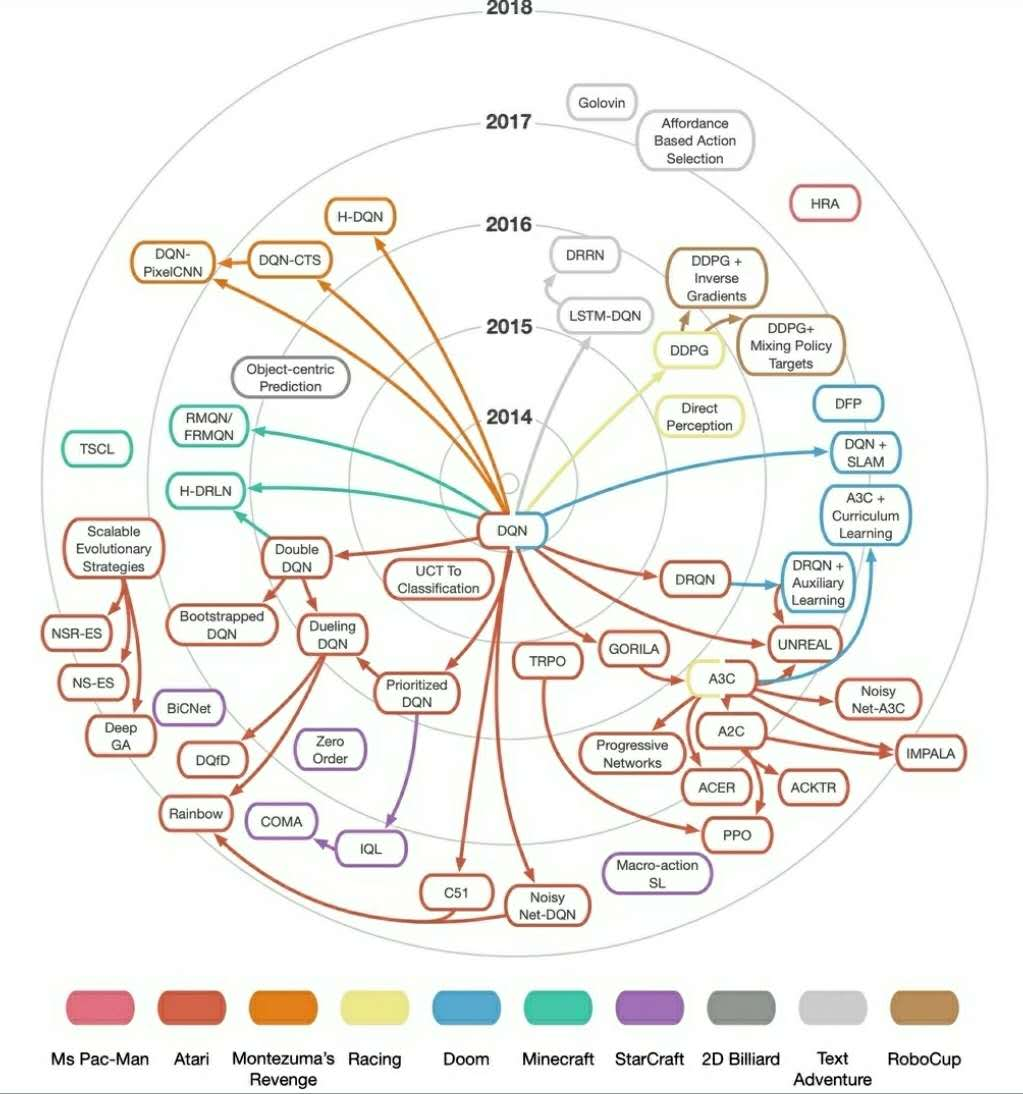
\includegraphics[scale=0.4]{img/rl.jpg}
	\caption{Reinforcement learning algorithms development.}
	\label{fig:rl}
\end{figure}

\textbf{REINFORCE}

REINFORCE \cite{williams1992simple} (or called vanilla policy gradient) is an algorithm using stochastic policy gradient method as in Eq.(\ref{equ:policy_gradient}), where the $\Phi_t = Q^\pi(s_t, a_t)$ and it is estimated with $V^\pi(s_t)=\sum_{t'=t}^{\infty}r_{t'}$ (or discounted version) in REINFORCE. The gradients for updating the policy are:
\begin{equation}
    g=\mathbb{E}[\sum_{t=0}^\infty \sum_{t'=t}^{\infty}r_{t'} \nabla_\theta \log \pi_\theta(a_t|s_t)]
\end{equation}
 
REINFORCE algorithm applies stochastic policy and updates the policy in an on-policy way. Although the estimation of $Q^\pi(s_t, a_t)$ using $V^\pi(s_t)$ is unbiased, but it could have large variance as a Monte-Carlo approach. More advanced approach like generalized advantage estimation (GAE) \cite{schulman2015high} could be applied to alleviate this problem in REINFORCE algorithm.

\textbf{Actor-Critic}

The actor-critic architecture is another approach for estimating the $Q^\pi(s_t, a_t)$ in policy gradient methods. Different from $V^\pi(s_t)$ in REINFORCE, the actor-critic applies an additional component called the critic for approximating the action-value function: $Q^\omega(s,a) \approx Q^\pi(s,a)$. The estimation of the critic could be biased but with lower variance compared with the REINFORCE algorithm. The gradients for updating the policy in actor-critic algorithm are:
\begin{equation}
    g=\mathbb{E}[\sum_{t=0}^\infty Q^\omega(s_t,a_t) \nabla_\theta \log \pi_\theta(a_t|s_t)]
\end{equation}
And the loss for the value evaluation function is difference of $Q^\omega(s,a)$ and the discounted rewards of corresponding time steps.

\textbf{Q-Learning}

Q-learning is a classical RL algorithm for discrete action space. And it has its deep learning variation which is Deep Q-Network. The key of Q-learning is to optimize the policy with the action-value function $Q(s,a)$, via the Bellman optimality equation for optimal action-value function $Q^*(s,a)$:
\begin{equation}
    Q^*(s_t,a_t) = \sum_{s_{t+1}}P^a_{s_t s_{t+1}}(r^{a_t}_{s_t s_{t+1}}+\gamma\max_{a_{t+1}} Q^*(s_{t+1},a_{t+1}))
\end{equation}
where the $P^{a_t}_{s_t s_{t+1}}$ is the probability of state transformation from $s_t$ to $s_{t+1}$ with action $a_t$, and $r^{a_t}_{s_t s_{t+1}}$ is the reward corresponding to that.
And the policy $\pi$ is represented as:
\begin{equation}
    \pi(s_t) = arg\max_{a_t} Q(s_t, a_t)
\end{equation}
The optimal action-value function can be derived with value iteration methods. The update rule for Q-learning is:
\begin{equation}
    Q(s_t,a_t) \leftarrow (1-\alpha)Q(s_t, a_t) + \alpha (r^{a_t}_{s_t s_{t+1}}+\gamma\max_{a_{t+1}} Q(s_{t+1},a_{t+1}))
\end{equation}
where $\alpha, \gamma$ are the step-size for soft update and the discount factor respectively.

\textbf{DQN}

Deep Q-Network (DQN) \cite{mnih2015human}\cite{mnih2013playing} applies deep neural networks in Q-learning for action-value function estimation. In order to realize that, DQN formalizes a differentiable objective function and derives the gradients for updating the policy:
\begin{equation}
\label{equ:dqn}
    g=\nabla_\theta \mathbb{E}_{s_{t+1}\sim P(s_{t+1}|s_t,a_t)}[(Q_\theta(s_t,a_t)-Q_{\theta'}^T (s_{t}, a_{t}))^2]
\end{equation}
where the target action-value function is represented by a target network with different parameters $\theta'$ for alleviating the problem of unstable target:
\begin{equation}
    Q_{\theta'}^T (s_{t}, a_{t}) = r^{a_t}_{s_t s_{t+1}}+\gamma\max_{a_{t+1}} Q_{\theta'}(s_{t+1},a_{t+1})
\end{equation}
Both the Q-learning and DQN work for discrete action space only. Their actions are all based on the argmax operation on the action-value function, instead of sampling from a stochastic policy.

\textbf{DDPG}

Deep deterministic policy gradient (DDPG) \cite{lillicrap2015continuous} is a combination of DQN and the actor-critic architecture with a deep deterministic policy (DPG) \cite{silver2014deterministic}. The deterministic policy is represented as $a_t=\mu_\theta(s_t)+\mathcal{N}_t$, which is different from the stochastic policy $\pi(a_t|s_t)$ in REINFORCE and actor-critic. The $\mathcal{N}_t$ is a noise term for exploration. And DDPG applies the two key points in DQN that could be effective: 1. the replay buffer and off-policy update; 2. the target networks.

The update rule for the critic in DDPG is the same as Eq.(\ref{equ:dqn}) in DQN. For the actor policy update in DDPG, it needs to replace the stochastic log-probability policy $\log \pi_\theta(s_t)$ in Eq.(\ref{equ:policy_gradient}) with the deterministic policy $\mu_\theta(s_t)$ of probability equivalent to 1 and parameterize the action-value function $Q(s,a)$ in Eq.(\ref{equ:policy_gradient}) with $\theta$ as $Q_\theta(s,a)$. By applying the chain rule, we can derive the update gradients for the actor network in DDPG:
\begin{equation}
    g\approx\frac{1}{N}\sum_i \nabla_a Q_\theta(s_i, a) \nabla_\theta(\mu_\theta(s_i))
\end{equation}
where $N$ is number of samples used for the update.

\textbf{TRPO}

Trust region policy optimization (TRPO) \cite{schulman2015trust} applies a surrogate loss for the policy update and makes the process of policy training a constrained optimization problem to achieve monotonically improvement in policy performance. The update rule for TRPO is:
\begin{equation}
\begin{aligned}
    \text{maximize}_\theta &\mathbb{E}_{s\sim \rho_{\theta_k}, a\sim\pi_{\theta_k}}[\frac{\pi_\theta(a|s)}{\pi_{\theta_k}(a|s)}A_{\theta_k}(s,a)]\\
    &\mathbb{E}_{s\sim \rho_{\theta_k}}[D_{KL}(\pi_{\theta_k}(\cdot|s)||\pi_\theta(\cdot|s))]\leqslant \delta
        
\end{aligned}
\end{equation}
where $\rho_\theta$ is the state-visitation frequencies and the advantage function $A(s_t, a_t)=Q(s_t, a_t)-V(s_t)$, and $\theta_k$ are parameters of the policy for after the $k$th update. TRPO has a more precise control about the policy update, but suffers from high computational cost because of the inverse of the Hessian matrix in the update steps.

\textbf{PPO}

Proximal Policy Optimization (PPO) \cite{schulman2017proximal} contains simplified approximations of TRPO algorithm for accelerating the computation process. It includes at least two versions of implementations with different approximations. The first approach is to apply an adaptive KL-divergence penalty instead of the constraint in TRPO:
\begin{equation}
    \text{maximize}_\theta &\mathbb{E}_{s\sim \rho_{\theta_k}, a\sim\pi_{\theta_k}}[\frac{\pi_\theta(a|s)}{\pi_{\theta_k}(a|s)}A_{\theta_k}(s,a)]-\beta \overline{KL}[\pi_{\theta_{old}}, \pi_\theta]\\
\end{equation}
The parameter $\beta$ for KL-divergence penalty is increased when the KL-divergence is large, and vice versa.

The second approach is to apply a clip surrogate optimization objective to replace the KL-divergence penalty in TRPO, which is more computationally efficient:
\begin{equation}
L^{CLIP}(\theta)=\mathbb{E}[\min(r_t(\theta)A_t, clip(r_t(\theta), 1-\epsilon, 1+\epsilon)A_t)]
\end{equation}
where the $r_t(\theta)$ denotes the probability ratio as $r_{t=k}(\theta)=\frac{\pi_\theta(a|s)}{\pi_{\theta_k}(a|s)}$. 

In practice, PPO algorithm usually shows more stable improvement in learning process compared with DDPG algorithm, but sometimes may learn slower. And more practical version of PPO algorithm like distributed PPO (DPPO) \cite{heess2017emergence} is proposed recently.

\textbf{A Comparison of Model-Free Reinforcement Learning Algorithms}

In table \ref{table:1}, we show a summary of different model-free RL algorithms on the aspects of on/off-policy and discrete/continuous action space. The RL algorithms include REINFORCE \cite{williams1992simple}, Cross-entropy method \cite{de2005tutorial}, general Actor-Critic, Advantage Actor-Critic (A2C) \cite{mnih2016asynchronous}, Asynchronous Advantage Actor-Critic (A3C) \cite{mnih2016asynchronous}, Actor-Critic with Experience Replay (ACER) \cite{wang2016sample}, Continuous Actor-Critic Learning Automation (CACLA) \cite{van2007reinforcement}, Q-Learning, Q-Prop \cite{gu2016q}, Deep Q-Network (DQN)\cite{mnih2015human}, SARSA, Deep Deterministic Policy Gradient (DDPG) \cite{lillicrap2015continuous}, Trust Region Policy Optimization (TRPO) \cite{schulman2015trust}, Proximal Policy Optimization (PPO) \cite{schulman2017proximal}, etc.

\begin{table}
    \centering
\begin{tabular}{ |c|c|c|c| } 
\hline
RL Algorithms & Policy & Action Space \\
\hline
{REINFORCE} & On-policy & Continuous\\
{CEM} & On-policy & Discrete and Continuous\\
{Actor-Critic, A2C, A3C, ACER}& On-policy & Discrete and Continuous\\
{CACLA}& On-policy & Continuous\\
{Q-Learning} & Off-policy & Discrete \\
{Q-Prop} & On-policy & Discrete and Continuous\\
{DQN} & Off-policy & Discrete \\  
{SARSA}& On-policy & Discrete \\ 
{DDPG} & Off-policy & Continuous\\
{TRPO} & On-policy & Discrete and Continuous\\
{PPO} & On-policy & Discrete and Continuous\\
\hline
\end{tabular}
\caption{Comparison of model-free reinforcement learning algorithms.}
\label{table:1}

\end{table}





\section{Environment}
\begin{figure}[htbp]
	\centering
	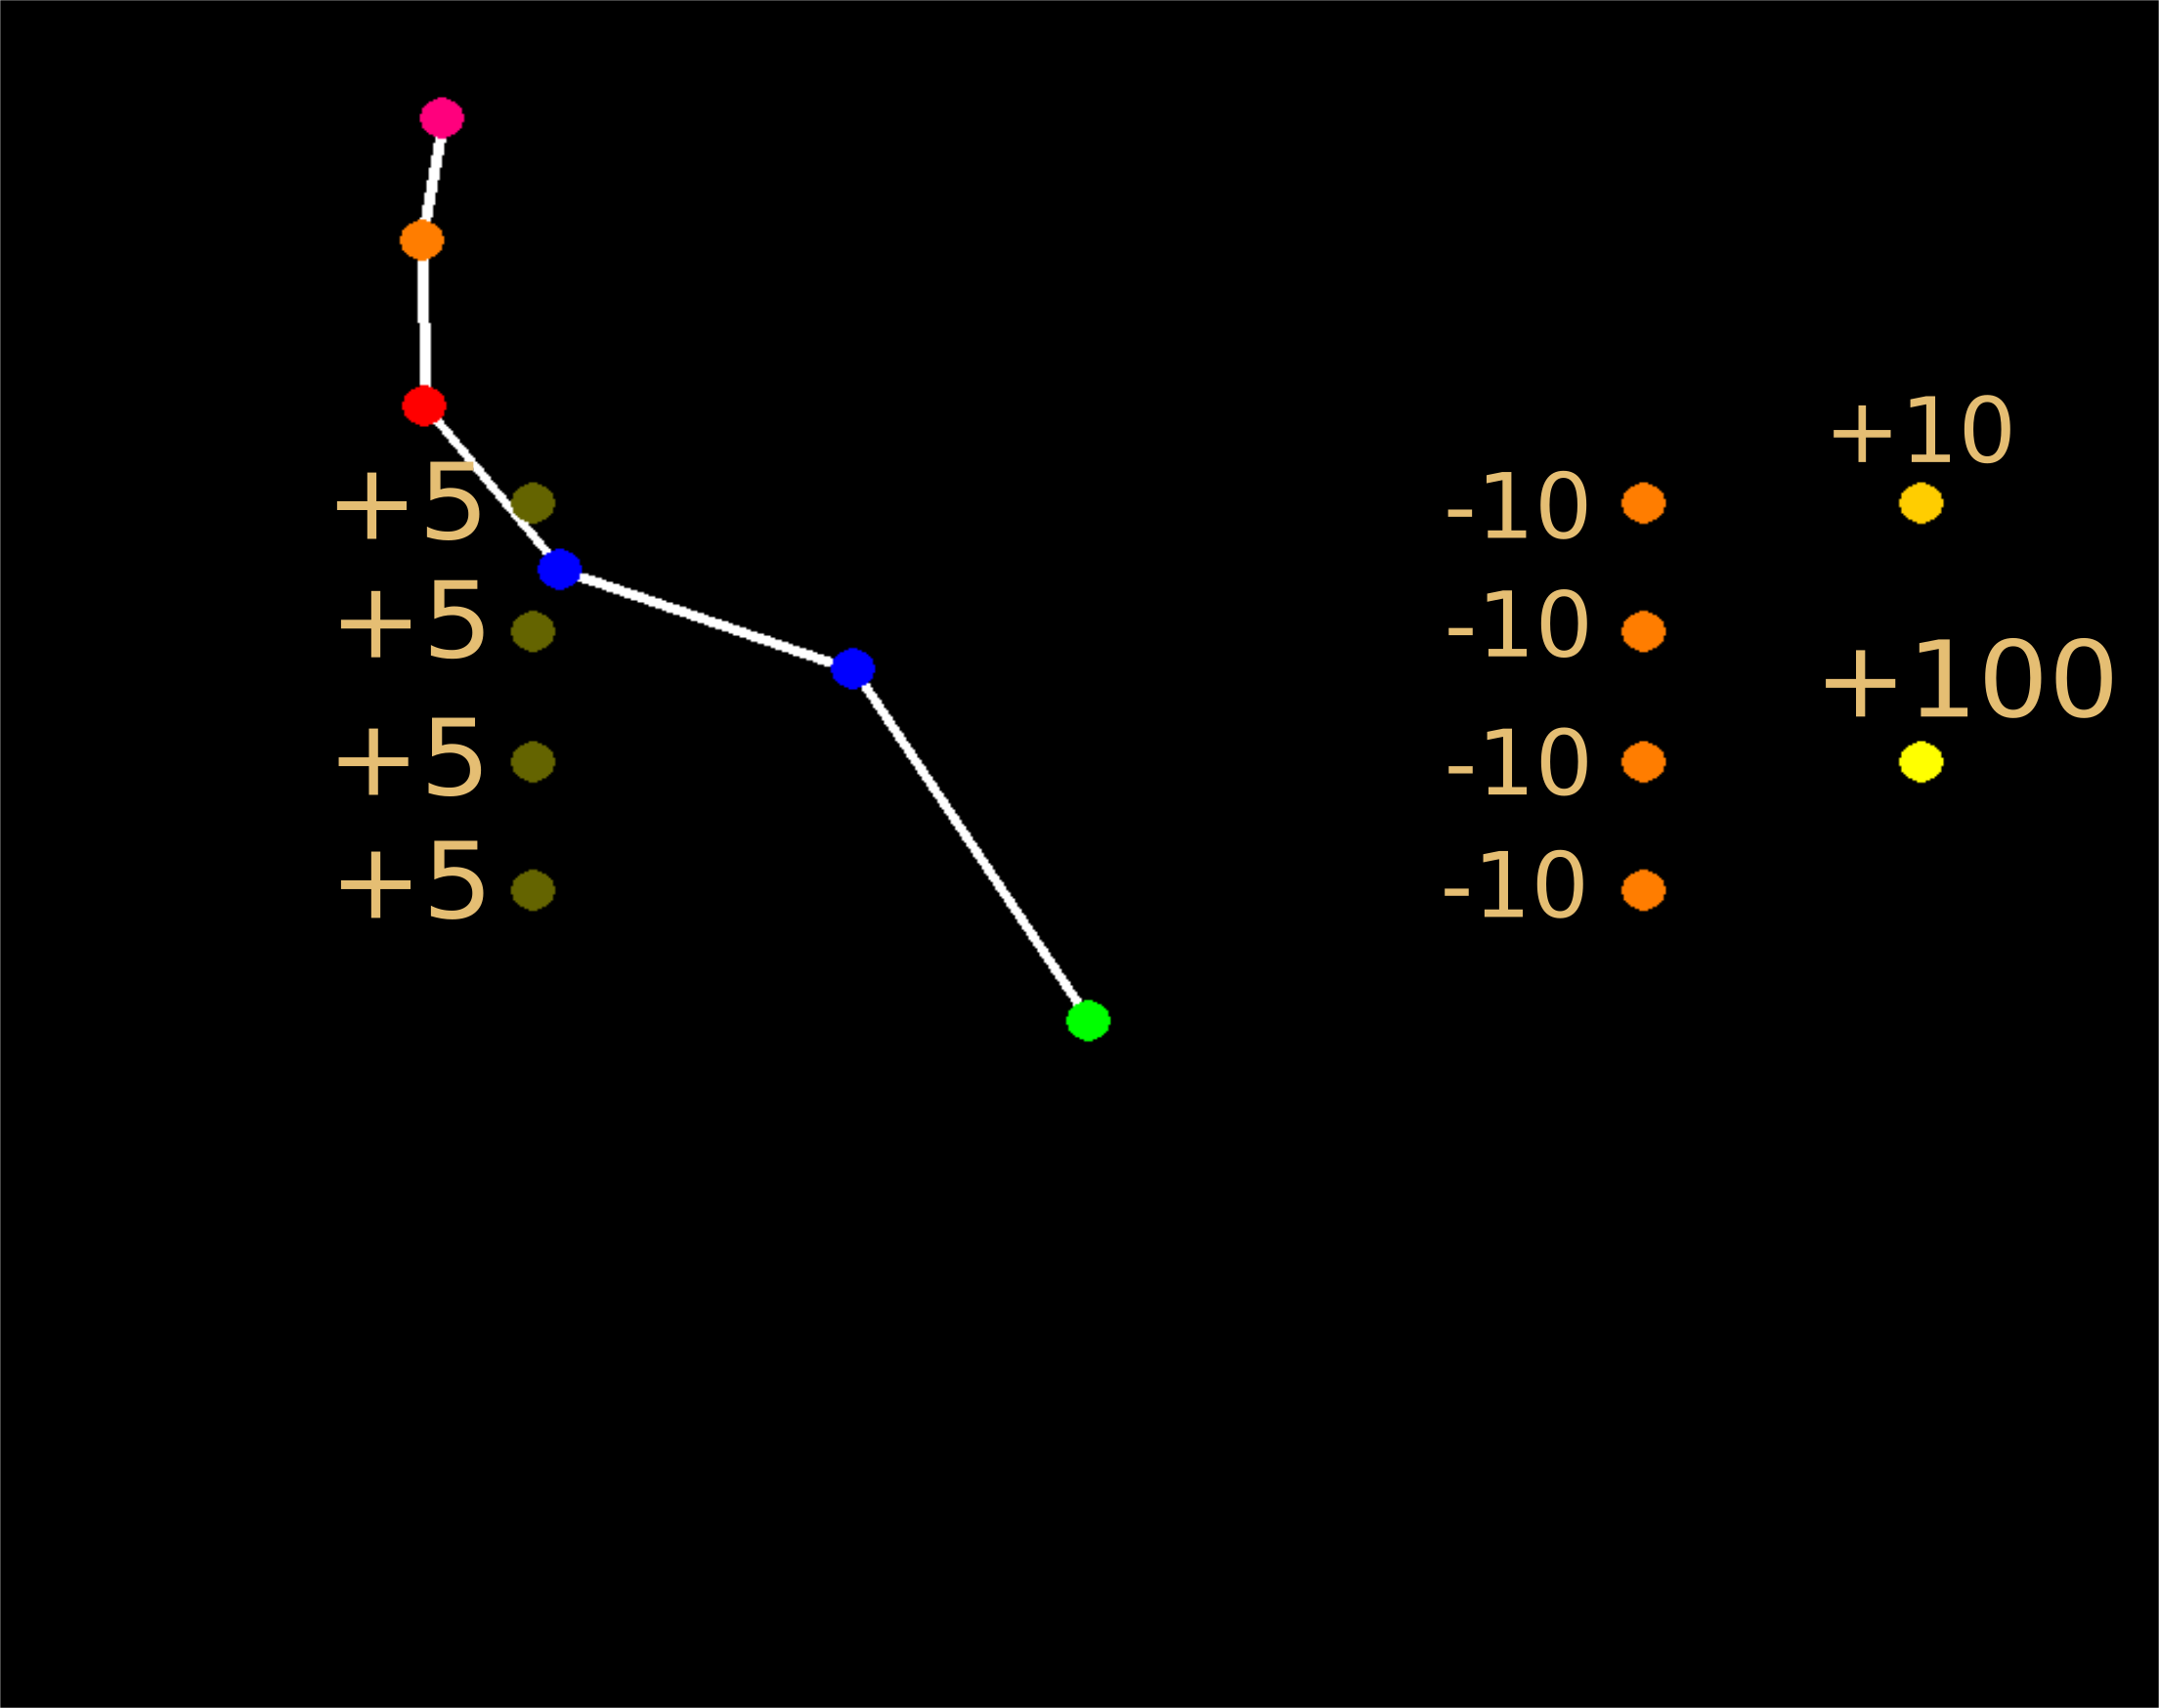
\includegraphics[scale=0.18]{img/reacher.png}
	\caption{\textit{Reacher} task with 5 joints and several reward/penalty positions}
	\label{fig:universe}
\end{figure}
In this work, we apply reinforcement learning algorithms on the \textit{Reacher} task. As shown in Fig.1, the goal of \textit{Reacher} task is to let the end position of `reacher'  agent to be as close as possible to the positions with highest rewards. The \textit{Reacher} task is a simplified environment very close to robotic arm control in reality, and this is the reason why we choose this environment in the research. Experiments in the following sections are all based on the \textit{Reacher} task, with slight modifications for different purposes.


\subsection{The \textit{Reacher} Task Specification}

The task space in our model is defined to be the same `reacher' structure with one target point at different positions. The number of joints of `reacher' is chosen to be 3 with length between each pair of joints to be 200, 140 and 100, respectively. The screen size is 1000 and the fixed start point of the `reacher' is at the center of the map. The target position is sampled from a random distribution within the allowed area.

\subsection{Reward Function}
The reward function is critical for a RL problem. It needs to satisfy at least two requirements: 

1. the reward function should match with the objective of the task, sometimes it's biased, but it at least has preferences for the optimization towards the objective.

2. the reward function should help with the optimization process for the policy of RL, which usually means it needs to be differentiable for a neural network approximator. 
\begin{figure}[htbp]
	\centering
	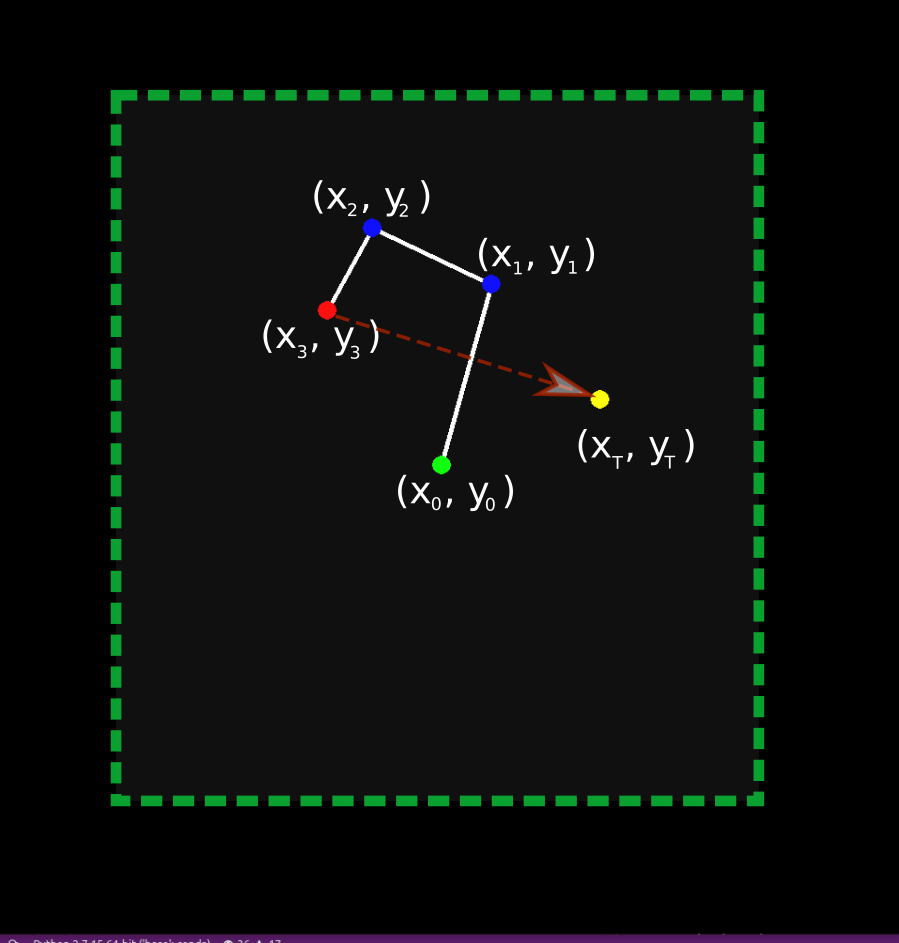
\includegraphics[scale=0.3]{img/reacher1.png}
	\caption{\textit{Reacher} task with three joints and one target point of different possible positions. The green dashed line is the area of potential target positions in the task space.}
	\label{fig:universe}
\end{figure}

There are usually two types of reward functions: the sparse reward and dense reward. A sparse reward is more close to the situations in real world tasks for human learning process, where the reward signals are rare. While in simulation learning task for RL, people tends to use the man-made dense reward functions for improving the learning efficiency. In practice, RL with sparse reward function could be hard to learn for the agent, techniques like Hindsight Experience Replay (HER) \cite{andrychowicz2017hindsight} can be applied to alleviate the problem when learning in multi-goal tasks like in \textit{Reacher} with random goal positions. 

The \textbf{dense reward} function for each step is defined as:
\begin{equation}
\label{equ:dense_reward}
 R=\frac{R_0}{\sqrt{(x_3-x_T)^2+(y_3-y_T)^2}+1}, 
\end{equation}
where $R_0=100$ is the maximum of reward value, so $R\in(0,100]$. $x_3, y_3$ is the end position of the reacher, and $x_T, y_T$ is the target position.

We could also use a \textbf{sparse reward} function as:
\begin{equation}
    R =
\begin{cases}
R_T& \sqrt{(x_3-x_T)^2+(y_3-y_T)^2}<r\\
-1& \text{Otherwise}
\end{cases}
\end{equation}
where $r$ is an arbitrary radius value (a precision factor) of the range we think the reacher has reached the goal, and $R_T$ is a constant reward of it.

In the following parts of this paper, experiments are conducted with the dense reward as default.

\subsection{Inverse Kinematics}
Inverse kinematics is a inverse process of forward kinematics, to derive the joint angle values with respect to the end position. Considering the end position as a transformation function of joint angels: $\mathcal{T}(\theta, L)$, where $\{\theta_i\}$ are joint angles and $\{L_i\}$ are link lengths, the forward kinematics is:
\begin{equation}
 (x_{end}, y_{end}) = \mathcal{T}(\theta, L)
\end{equation}
while the inverse kinematics needs the Jacobian of end position with respect to the joint angles parameters $\{\theta_i\}$, and to reach a specific target position $(x_T, y_T)$ from $(x_{end}, y_{end})$, the expected change of angle values are:
\begin{equation}
	\Delta \theta = \alpha (\frac{\partial(\mathcal{T}(\theta, \L))}{\partial \theta})^{-1} \cdot [(x_T, y_T)-(x_{end}, y_{end})]
\end{equation}
where $\alpha$ is the step size. 

And in practice, we usually use Moore–Penrose pseudo-inverse for calculation of the inverse Jacobian, which will induce approximation error in trajectories.





\section{Efficient Reinforcement Learning with Demonstrations}

\subsection{Approaches of Demonstrations Generation}
A good demonstration is a pre-collected trajectory for the agent to have relatively large rewards in the episode. By leveraging good demonstrations with proper methods, reinforcement learning can learn faster and robuster through imitating or drawing lessons from them. It could be extremely useful for training robotics in reality, where the training cost could be huge practically.
There are at least three approaches for generating the demonstrations:

1. \textbf{Model-based reinforcement learning}. Model-based reinforcement learning can efficiently train a policy with small numbers of samples, like model predictive control (MPC) \cite{nagabandi2018neural}. The learned policy can be used to initialize a model-free reinforcement learning model with supervised imitation learning.

2. Analytic-form solutions like \textbf{inverse kinematics}. For \textit{Reacher} environment, we can analytically calculate the action values to generate a trajectory reaching the goal, with the method of inverse kinematics described in the above section. Demonstrations can be collected in simulation with inverse kinematics. Details are shown in the below section.

3. \textbf{Human expert demonstrations}. Above two approaches can be solved in simulation, but in reality, it could be hard to either model the real world environment or solve a analytic solution for it. The most direct way to generate good demonstrations in reality is to collect demonstrations from human experts \cite{bojarski2016end}. However, this could be expensive in both human-labor and time consumption, therefore the number of demonstrations from human is supposed to be smaller, compared with those demonstrations generated in simulation.


\subsection{Imitation Learning with Demonstrations}
In this section, we introduce different approaches for learning a policy with demonstrations, which is a problem known as \textbf{imitation learning}. Three basic approaches of imitation learning including supervised learning, inverse reinforcement learning and generative adversarial imitation learning are summarized. 

The basic setup for applying imitation learning is to learn a policy without any reinforcement signals but only the demonstrations data, which means the learned policy through imitation learning is the final policy from the demonstrations. However, in our problem formalization, the reinforcement signals can still be provided after the imitation learning process, and the RL learning takes the policy learned from imitation learning as an initialization. Therefore, we do not require the policy from imitation learning to be optimal, but good enough with a relatively simple imitation learning process, like the supervised approach. So we only choose some of the simple and straightforward methods in those approaches described below as initialization method for subsequent RL process. Those fancy techniques in imitation learning will provide a better initialization policy with no doubts, but it's not what we focus on.

\subsubsection{Supervised Learning Approach}
The imitation learning with demonstrations can be naturally regarded as a supervised learning problem. Consider an initialization policy $\pi_{ini}$ parameterized by $\theta$ with input state $s$ and output action $a$ in a RL setting, we have demonstrations dataset $\mathcal{D} = \{(s_i, a_i)\}$ generated from above approaches, which could be used to train the policy, with an objective as follows:
\begin{equation}
\label{equ:bc}
    \min_{\theta}\frac{1}{2}\sum_{(s_i, a_i)\sim \mathcal{D}}||a_i- \pi_{ini}(s_i)||^2_2
\end{equation}
This supervised learning approach to directly imitating the demonstrations is sometimes called the \textbf{behavioural cloning (BC)} or policy replacement in this paper.

\textbf{DAGGER}

DAGGER \cite{ross2011reduction} is a more advanced no-regret iterative algorithm for imitation learning from demonstrations. It proactively choose demonstration samples that the policy has larger chances to meet afterwards according to the previous training iterations, which makes DAGGER more effective and efficient for online imitation learning in sequential prediction problem like RL.

\textbf{Variational Dropout}

Another method for alleviating generalization problem in imitation learning is pre-training with variational dropout \cite{blau2018improving}, instead of cloning the behavior of expert demonstrations in policy replacement (or called behavioural cloning, BC) methods. Variational dropout \cite{molchanov2017variational} can be taken as a more advanced method for generalization than noise injection in the weights of trained neural networks, it reduces the sensitivity of choosing the magnitude of noise.

\textbf{Others}

Although imitation learning can show a relatively good performance for sequential prediction problem for those samples similar to the dataset the policy is trained with, it will suffer from bad performances for those samples it never meet before, especially in a scenario like RL. Some methods provide a way to generalize demonstrations to more general scenarios in a task using framework like \textbf{dynamic movement primitive (DMP)} \cite{pastor2009learning} in an analytic form, but these methods are restricted in applications with simple analytic-form descriptions like robot arm controls. And method in one-shot imitation learning \cite{duan2017one} uses \textbf{soft attention} on demonstrations to generalize model to unseen scenarios in training data. It is a meta-learning scheme to map one demonstration of one task to an effective policy for the task. 

\subsubsection{Inverse Reinforcement Learning Approach}
Inverse reinforcement learning (IRL) \cite{ng2000algorithms} \cite{russell1998learning} is to extract a reward function from observed optimal behavior, like the expert demonstrations in our problem, or say to find a loss function under which the observed trajectories is optimal. A typical IRL method is maximum causal entropy IRL \cite{ziebart2008maximum}, which tries to learn a cost function $c(s,a)$ with the objective of maximizing the causal entropy:
\begin{equation}
    \max_c(\min_\pi -\mathbb{E}_\pi[-\log \pi(a|s)]+\mathbb{E}_\pi[c(s,a)])-\mathbb{E}_{\pi_E}[c(s,a)]
\end{equation}
where the $\pi_E$ denotes the expert policy for generating expert demonstrations and $\pi$ is the policy used in RL process. The learned cost function will assign high-entropy to expert policy and low-entropy to other policies.

And an optimal policy can be learned with with the learned cost function with the following formula:
\begin{equation}
    RL(c)=\arg \min_{\pi} -H(\pi)+\mathbb{E}_{\pi}[c(s,a)]
\end{equation}
With above methods, the IRL could learn a better policy from demonstrations and interactions in the general RL process. However, the computational cost could be considerable with IRL-based methods.

\subsubsection{Generative Adversarial Approach}
The generative adversarial imitation learning (GAIL) \cite{ho2016generative} applies a discriminator in generative adversarial networks (GAN) for providing the estimation of action-value function based on demonstrations. In a general process of action-value based RL with algorithms like TRPO, PPO, etc, the action-value is provided from the demonstrations with a generative approach as:
\begin{equation}
    Q(s,a)=\mathbb{E}_{\mathcal{T}_i}[\log(D_{\omega_{i+1}}(s,a))]
\end{equation}
where  $\mathcal{T}_i$ are samples from RL's explorations and $D_{\omega_{i+1}}(s,a)$ is the output value from the discriminator with parameters $\omega_{i+1}$.
And the loss function of the discriminator is defined in a general way:
\begin{equation}
    \mathbb{E}_{\mathcal{T}_i}[\nabla_\omega\log(D_\omega(s,a))]
    +\mathbb{E}_{\mathcal{T}_E}[\nabla_\omega\log(1-D_\omega(s,a))]
\end{equation}
where the $\mathcal{T}_i, \mathcal{T}_E$ are samples from RL's explorations and expert demonstrations respectively. $\omega$ are parameters of the discriminator.

With the method of GAIL, the policy can be learned with samples generalized from demonstrations with lower computational cost, compared with methods via inverse RL. And it does not need to interact with the expert during training, which happens in method like DAGGER and is sometimes not accessible in practice.

Multi-modal imitation learning with GAN \cite{hausman2017multi} applies a fancier objective function with a generative adversarial form, to automatically segment the demonstrations for different tasks and learn a multi-modal policy.

\subsubsection{Supervised Imitation Learning as an Initialization for Reinforcement Learning}
As described in the beginning of this section, we only need to use those simple but effective methods in imitation learning as initialization of a subsequent RL process. And the methods we apply are mainly within the supervised learning approach. 

Generally, the policy learned from imitating the demonstrations, including the \textbf{BC, DAGGER, Variational Dropout and so on},  can be regarded as a good initialization for RL policy, using methods like \textbf{policy replacement or residual policy learning} described in the following sections. And we will experimentally show the improvement in RL with the initialization policy trained using above mentioned supervised learning methods in the following sections.

\subsection{Initialized Reinforcement Learning with Supervised Learning Policy -- Policy Replacement}

Reinforcement learning algorithms usually take a long time to achieve a good policy for a specific task. And the policy always needs to be re-trained if the settings of the task are changing, even if slightly. 

There are several ways to improve the learning efficiency of reinforcement learning algorithms. One promising way is to initialize the reinforcement learning policy with a pre-trained policy, in a manner of \textbf{policy replacement}, like cloning the behaviours of demonstrations. \textbf{The pre-trained policy with supervised learning approach described in the last section is used to replace the policy in RL as an initialization.} And this is especially effective when the pre-trained policy is trained on a similar task with the one the reinforcement learning is trying to solve. Moreover, if the pre-trained policy is trained across the task space containing all possible settings of a specific task that the RL is solving, it can leverage the learning performance of RL for all tasks defined in this task space.

In our model, we try to initialize RL with sub-optimal policy pre-trained before the RL process, and the policy is trained with supervised learning with expert trajectories sampled from inverse kinematics on \textit{Reacher} tasks. 


\subsubsection{Pre-trained Policy with Supervised Learning}
We apply a neural network of 5 layers to train an initialization policy, with the data generated from inverse kinematics. The inputs of neural network are positions of joints and position of the target.  Each hidden layer contains 100 nodes and uses ReLu as activation function. The output layer is Tanh activated with a scaling factor of 360, to make outputs range from -360 to 360 degree as a reasonable action value of the joints. The AdamOptimizer is applied with stochastic gradient descent in the training process. The training curve is shown in Fig. 3. Note that the y-axis is transformed to be in range [-1,1] instead of [-360, 360] as the mean squared error per action value .
\begin{figure}[htbp]
	\centering
	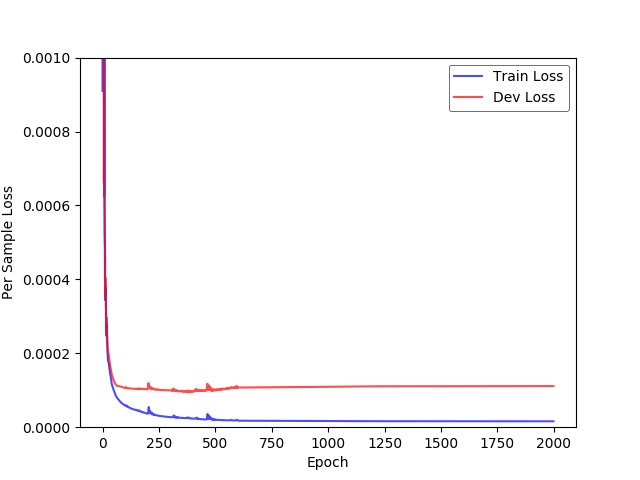
\includegraphics[scale=0.8]{img/supervised.png}
	\caption{Training curve of supervised learning with data from inverse kinematics.}
	\label{fig:universe}
\end{figure}

Here are several specifications about following experiments: (1). whenever there is a preheating process, the initial 600 steps in the learning curves are only for updating the critic (no actor update), so there is very small variance in learning curves when the noise applied is small; (2). as we are exploring the initialized policy for RL learning process, we only show experiments about the initial training steps (e.g. 2000 steps) for displaying the initialization effects.

\subsubsection{Policy Replacement as Initialization}
Policy replacement is one approach to apply the policy from supervised learning in initialization of RL. The basic idea is to use the same network structure in supervised learning and the actor in RL, so that a copy can be made from the supervised learning policy to the actor as an initialization of RL. Some tricks can be applied in this process to guarantee a performance improvement, like the preheating process. 

However, potential problems exist in policy replacement approach for initialization of RL, e.g. the initialized policy is fragile in the initial training process even with small exploration noise scale, which means the initialized good policy may degrade to some worse polices (the decrease on learning curve at initial training stage) and get improved through a re-learning process. We analysed the reason for the problems and proposed some strategies for solving or alleviating it. Further analysis seen in the following subsections.

\subsubsection{DDPG with Policy Replacement}
\textbf{General Process}

We apply the DDPG algorithm for the task, and show the comparisons with or without initialization for the policy.

The DDPG algorithm contains four neural networks: the actor network, the critic network, the target-actor network, and the target-critic network. For initializing the DDPG, we define the actor network and target-actor network to have exactly the same structure as the network in supervised learning. 

Initialization process of DDPG with supervised learning policy are as follows: 
(1). the weights of pre-trained supervised learning policy are loaded into the actor network and the target-actor are updated immediately; (2). samples are generated with initialized but frozen actor network with noise to pre-train the critic network; (3). train both the actor and critic network (also the target-actor and target-critic networks). Experiments show that the second step is non-trivial process for effective training DDPG with initialization. Details are explained in Sec. \ref{pretrain}.

Comparison of initial learning performances of DDPG with and without initialization policy on \textit{Reacher} task are shown in Fig. 4. The DDPG with initialization policy could significantly outperforms the one without initialization. 

\begin{figure}[htbp]
	\centering
	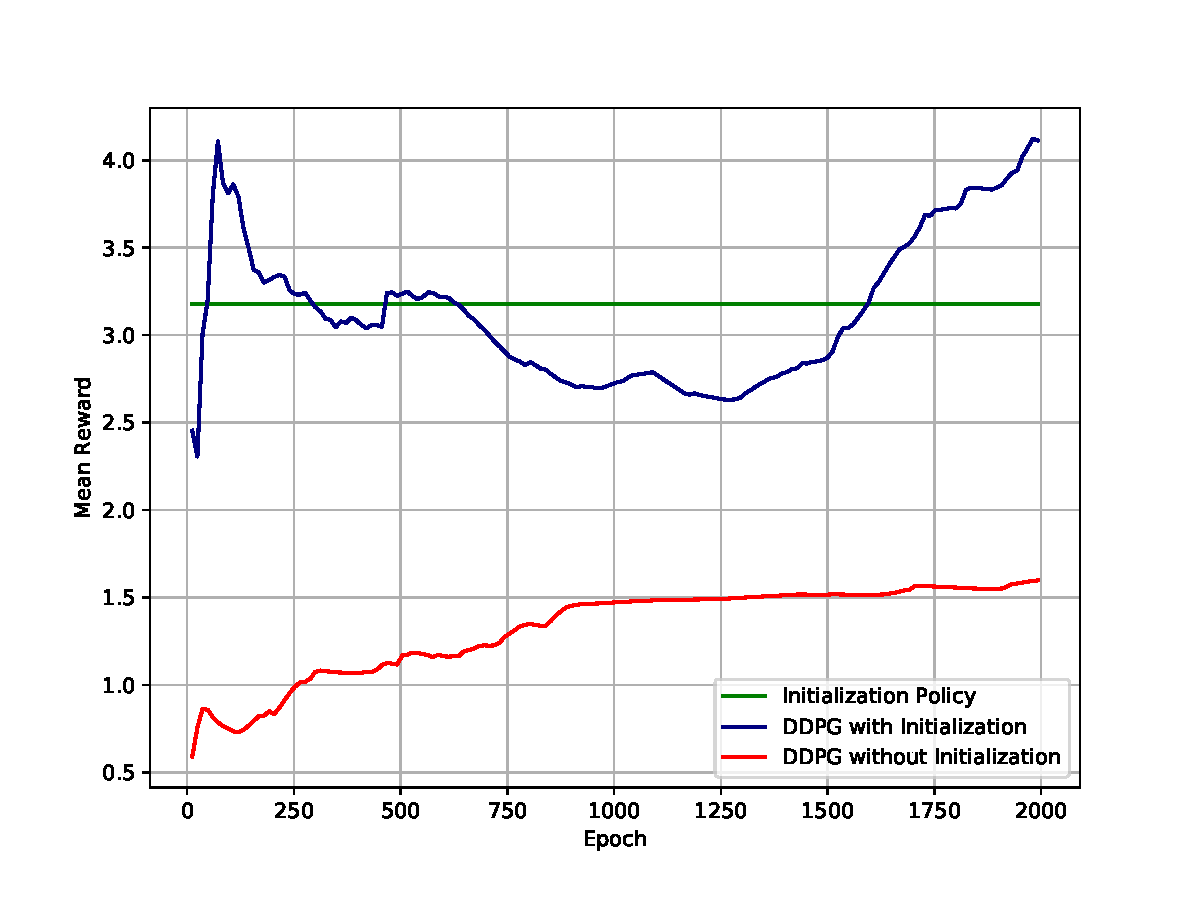
\includegraphics[scale=0.5]{img/ddpg_compare1.pdf}
	\caption{Comparison of initial learning performances of DDPG with/without initialization policy on \textit{Reacher} task. The green line is the mean reward of initial policy trained with supervised learning. The blue line and red line are mean rewards of DDPG with and without initialization in initial 2000 training epochs . }
	\label{fig:universe}
\end{figure}

There are several key components in initializing the RL with supervised learning policy affecting the performance of initialized RL (DDPG), including the scale of action noise in initialized RL, different ways of normalization in supervised learning and RL, learning rates of the actor and the critic in initialized RL, number of steps of single episode and so on. Improper settings of all above factors will affect the initialization policy to be effective for RL process. Some general intuitions about making the initialization more effective for RL are like: ensuring the inputs and outputs of the replaced policy from initialization to be as similar as possible between the supervised learning and RL, therefore applying the same input and output normalization to make sure they are of the same ranges of value, the same initial positions for each episode in `Reacher' and the same maximum length of single episode in supervised learning and RL, etc. 

\textbf{Choice of Noise}

\begin{figure}[htbp]
	\centering
	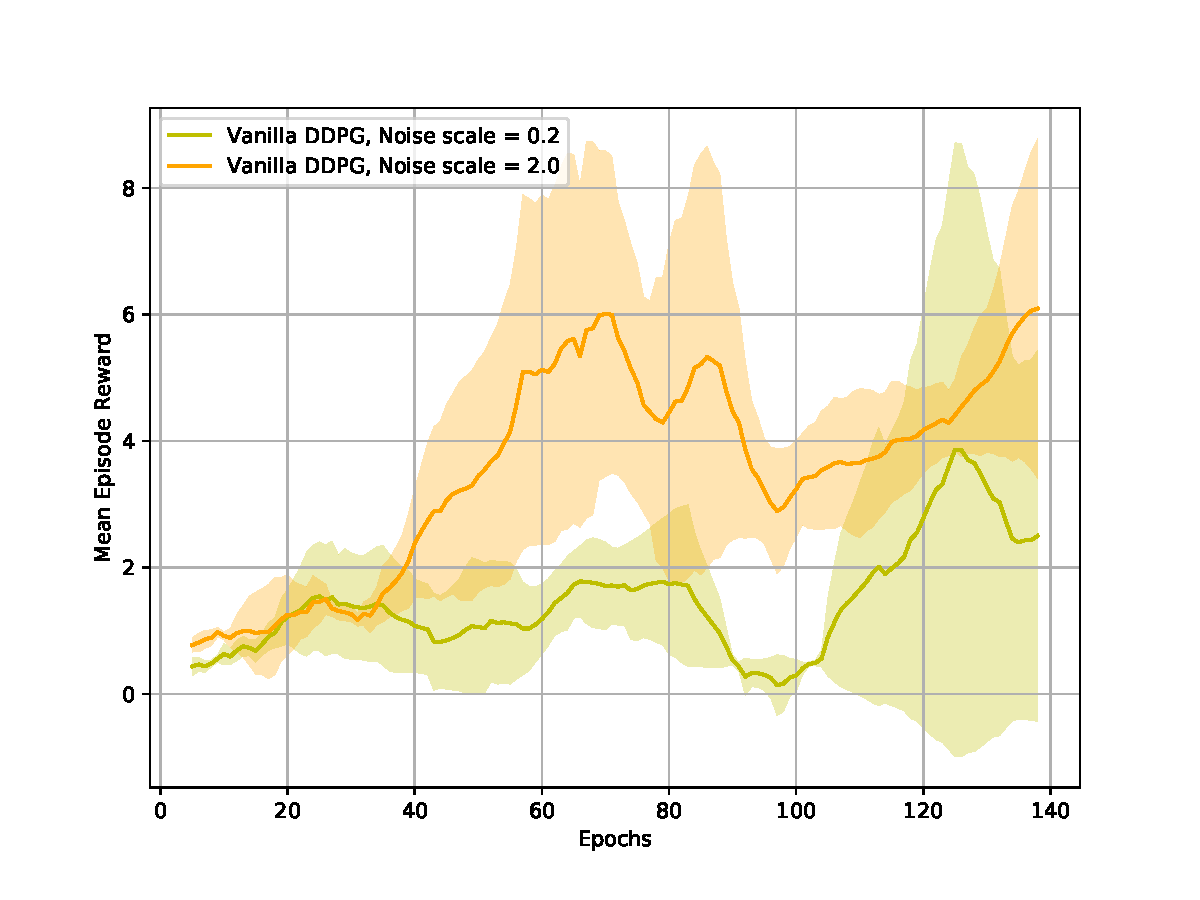
\includegraphics[scale=0.5]{img/3000step1.pdf}
	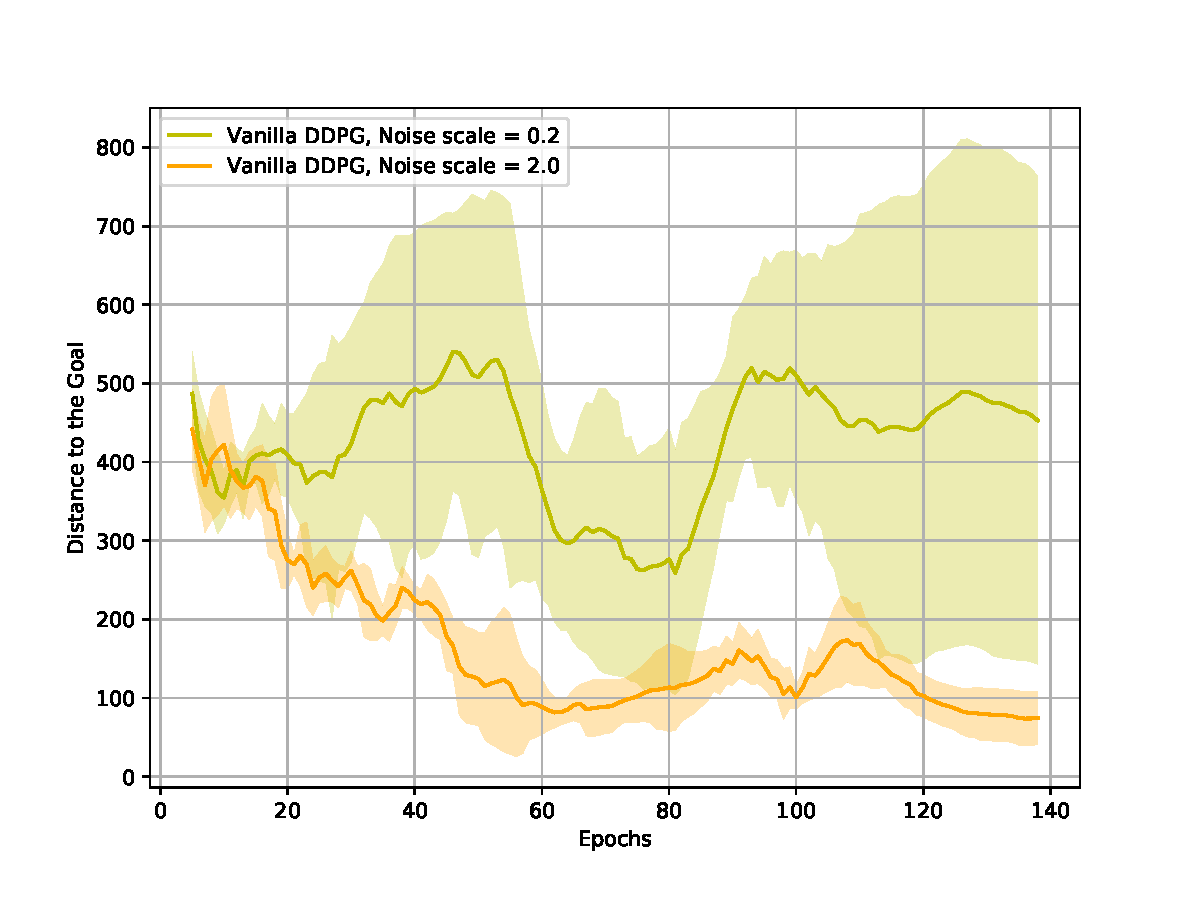
\includegraphics[scale=0.5]{img/3000step2.pdf}
	\caption{The effects of different noise scale for vanilla DDPG algorithm on \textit{Reacher} tasks. The experiments are conducted with general settings. The figure on the top shows the changing of mean episode reward during training, and the one below shows the changing of distance of the reacher's end to the goal position. }
	\label{fig:noise0}
\end{figure}

Noise is an important factor for RL learning process. As shown in Fig. \ref{fig:noise0}, different noise scales affect the performance of DDPG algorithm on \textit{Reacher} tasks greatly. For initialized policy $\pi_i$ trained with expert trajectories, the optimal trajectory for the same task should be some neighboring trajectories of the initialized trajectory, which means the difference of optimal policy $\pi^*$ and $\pi_i$ should be within a small range $\Delta$,
\begin{equation}
	D_{KL}(\pi^*||\pi_i)<\Delta
\end{equation}
This can be derived easily by $(\pi^*(a^*|s_t)- \pi_i(a^*|s_t))<\delta$, where $a^*$ is the optimal action for state $s_t$. However, if we consider another initial policy $\pi'_i$ which is not as good as $\pi_i$, then $(\pi'^*(a^*|s_t)- \pi_i(a^*|s_t))<\delta'$ and $\delta'>\delta$, also we have $D_{KL}(\pi^*||\pi'_i)<\Delta'$ and $\Delta'>\Delta$. In order to handle different initialization policies like $\pi$ or $\pi'$, we need to apply different noise for a better learning performance.

Generally, a larger noise scale or larger probability to have a noise action will help worse policy $\pi'$ to have larger chances to sample an optimal action. We can testify the case of larger probability of have a noise through $\epsilon$-greedy policy, as shown in Fig. \ref{fig:noise}. The $\epsilon$-greedy policy is defined as follows:
\begin{equation}
\pi(a|s)=\left\{
\begin{aligned}
&1-\epsilon+\frac{\epsilon}{|A(s)|}, &a=a* \\
&\frac{\epsilon}{|A(s)|}, &a\neq a*
\end{aligned}
\right.
\end{equation}

\begin{figure}[htbp]
	\centering
	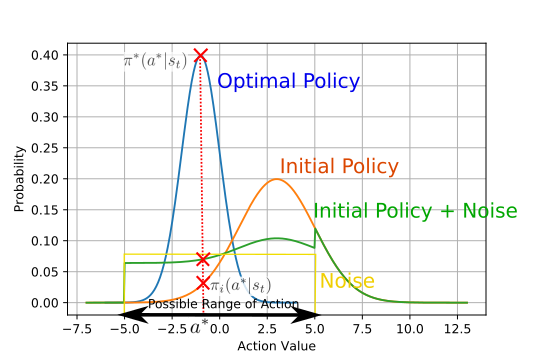
\includegraphics[scale=0.8]{img/noise2.png}
	\caption{A figure showing why adding noise would help for exploring better actions, with noise type of $\epsilon$-greedy policy. Suppose the initial policy and the optimal policy are Gaussian distributions with different means and variances, and the noise is a uniform distribution within specific range (range of possible action value). The figure shows how the noise of $\epsilon$-greedy helps to increase the possibility for non-optimal policy to sample the optimal action }
	\label{fig:noise}
\end{figure}

In Fig. \ref{fig:noise}, the $\epsilon$-greedy policy can be regarded as a uniform distributed noise on the possible range of action value. It shows that the noise helps the initial policy to have a larger probability to sample the optimal action $a^*$, when the initial policy has a relatively large difference from the optimal policy, which is the case of $\pi'$ with the KL-divergence upper bound  $\Delta'>\Delta$. Fig. \ref{fig:noise1} shows that for the same optimal distribution and different initial distributions, same $\epsilon$ will cause different effects for noisy policy. Generally, it shows that large $\epsilon$ value (0.8) only helps with large divergence of initial policy and optimal policy. And this is the reason to apply decayed $\epsilon$ in practice for $\epsilon$-greedy policy.

Fig. \ref{fig:noise2} shows that when two policies have large divergence $\Delta'$, larger $\epsilon$ in will help more for the initial policy to sample optimal actions with $\epsilon$-greedy policy. And larger $\epsilon$ generally means larger chances to have noisy actions.

\begin{figure}[htbp]
	\centering
	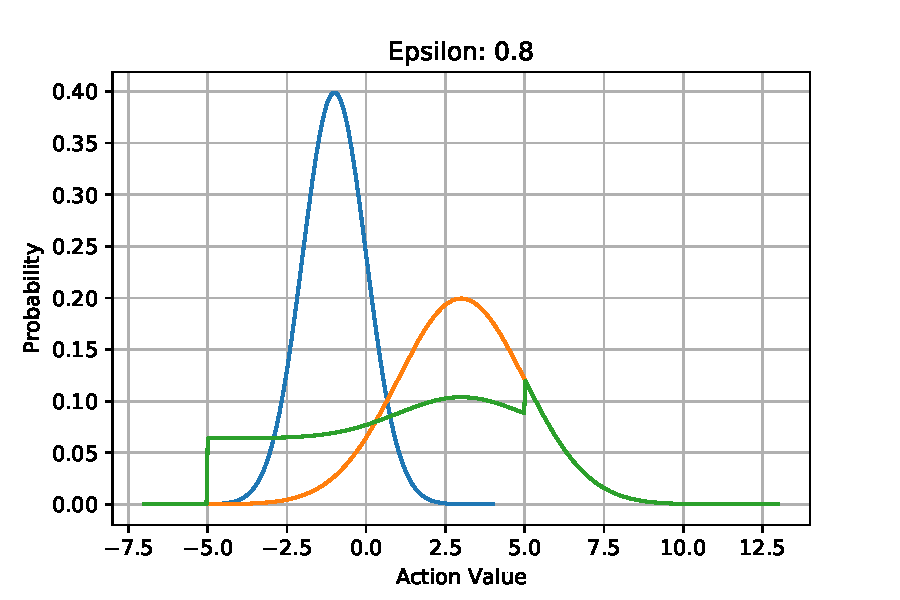
\includegraphics[scale=0.4]{img/noise28.pdf}
	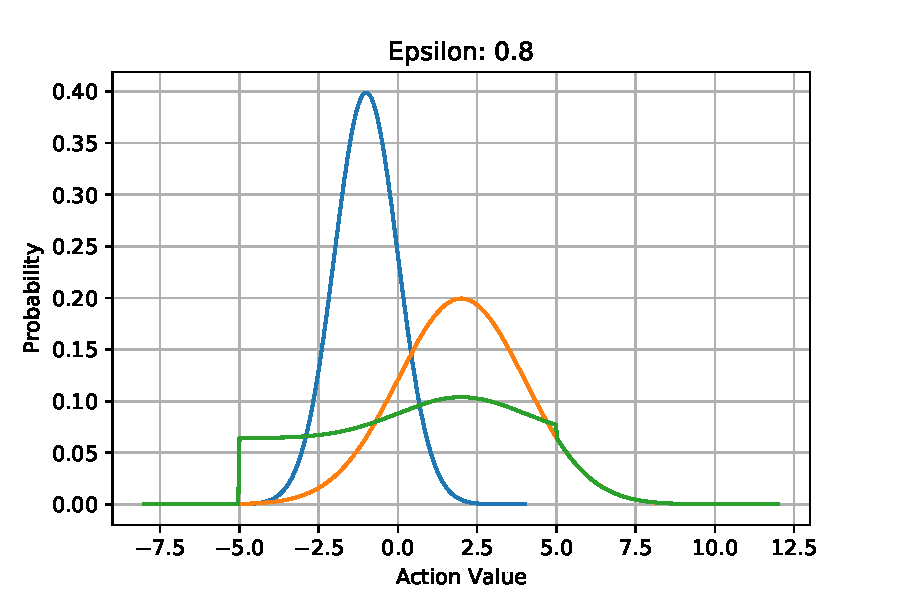
\includegraphics[scale=0.4]{img/noise38.pdf}
	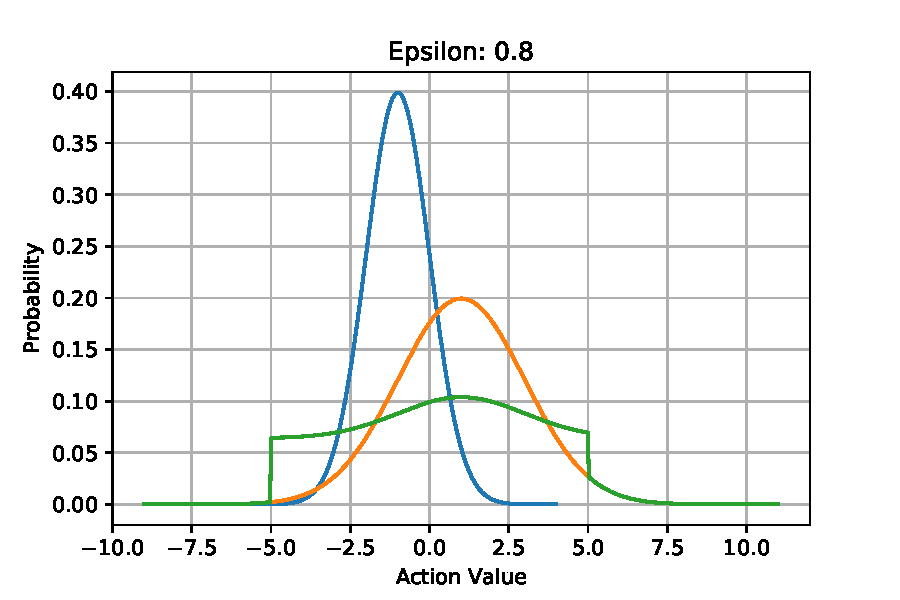
\includegraphics[scale=0.4]{img/noise48.pdf}
	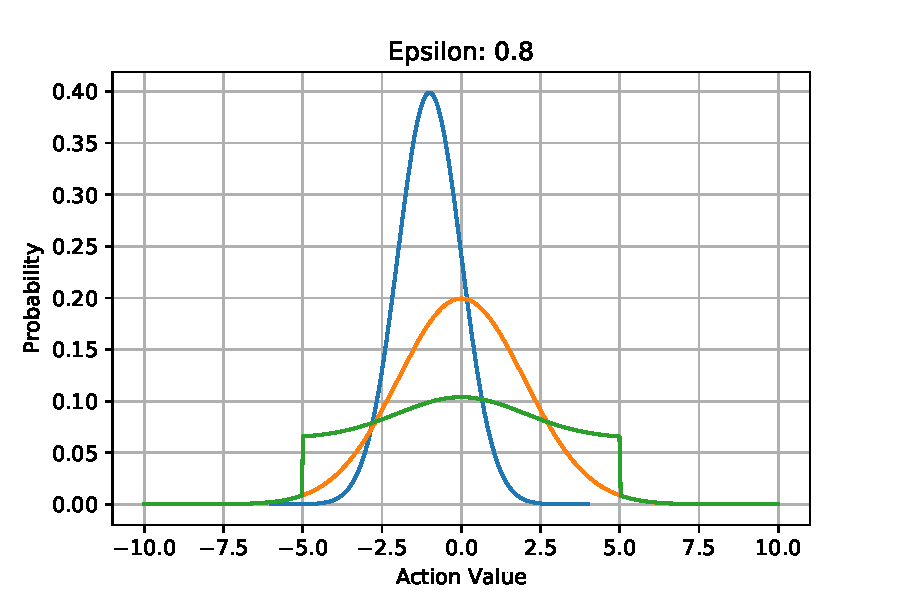
\includegraphics[scale=0.4]{img/noise58.pdf}
	\caption{$\epsilon$-greedy policy with different initial distributions and same $\epsilon$ value. It shows the same $\epsilon$ will cause different effects for noisy policy, it benefits the top two initial distribution and hurts the bottom two distributions. So large $\epsilon$ value (0.8) only helps with large divergence of initial policy and optimal policy. }
	\label{fig:noise1}
\end{figure}

\begin{figure}[htbp]
	\centering
	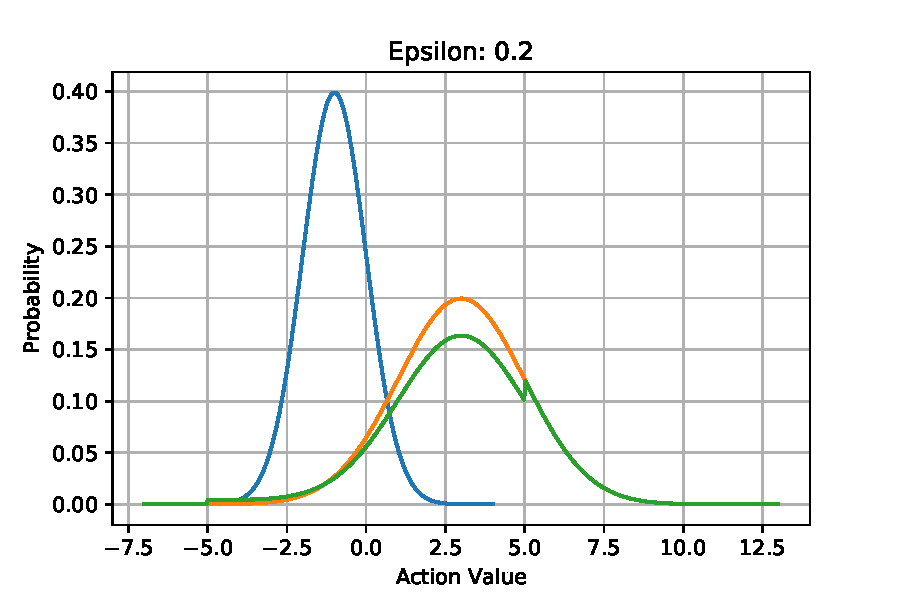
\includegraphics[scale=0.4]{img/noise22.pdf}
	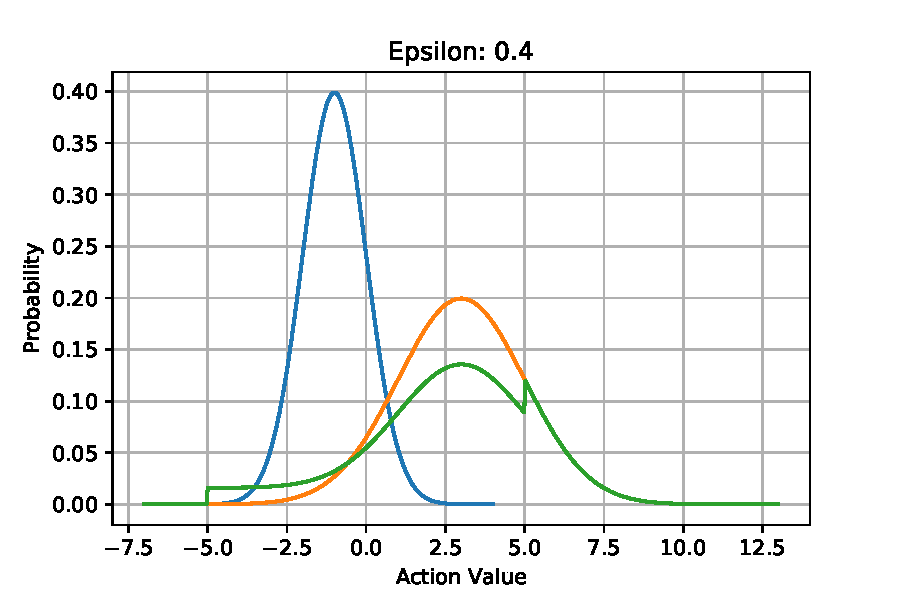
\includegraphics[scale=0.4]{img/noise24.pdf}
	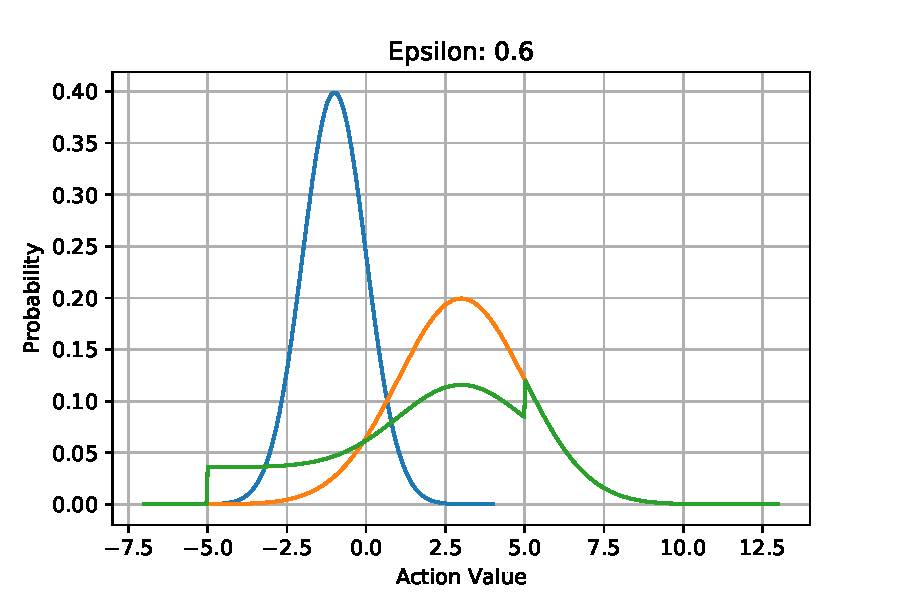
\includegraphics[scale=0.4]{img/noise26.pdf}
	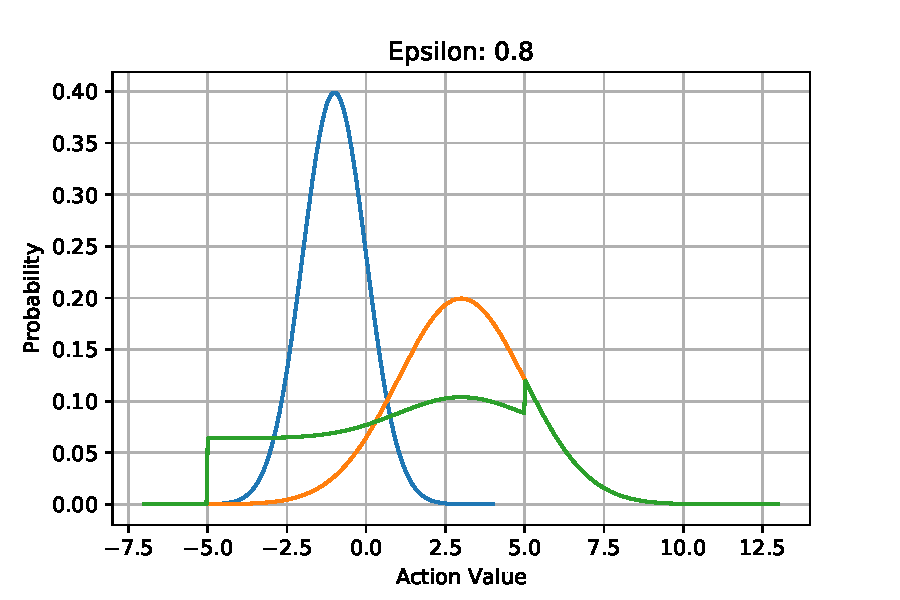
\includegraphics[scale=0.4]{img/noise28.pdf}
	\caption{$\epsilon$-greedy policy with different $\epsilon$ value and same initial and same optimal distribution. Larger $\epsilon$ value benefits more for large divergence between the optimal policy and the initial policy. }
	\label{fig:noise2}
\end{figure}
Above analysis is based on $\epsilon$-greedy policy, which represents the variety of probability to apply the noise in actions. However, the case of the variety in scale of noise has similar effects for different distributions. Therefore, we can derive some conclusions that for better initial policy, it means the smaller the divergence it is from the optimal policy, therefore it needs to apply noise with a smaller probability or apply smaller scale noise. So, how does it work in initialized RL?


In initialized RL, the cases are the same. Experiments with different initialized policy for DDPG on \textit{Reacher} task are shown in Fig. \ref{fig:noise3}, in which the relatively good initial policy $\pi$ is called from expert, and the relatively bad but better than random initial policy $\pi'$ is called the half-expert. Fig. \ref{fig:noise3} shows that for a bad initial policy, which has a relatively large divergence from the optimal policy, larger noise scale works better for improving the learning performance. And this results testify the above analysis of the case of $\epsilon$-greedy policy. Note that the experiments shown in Fig. \ref{fig:noise3} are all without preheating process, which is the second step described in the general process section. However, if we take experiments on the policy initialized from a better policy, Fig. \ref{fig:noise4} shows smaller noise is better for DDPG initialized with an expert policy, which also testifies above analysis results.
\begin{figure}[htbp]
	\centering
	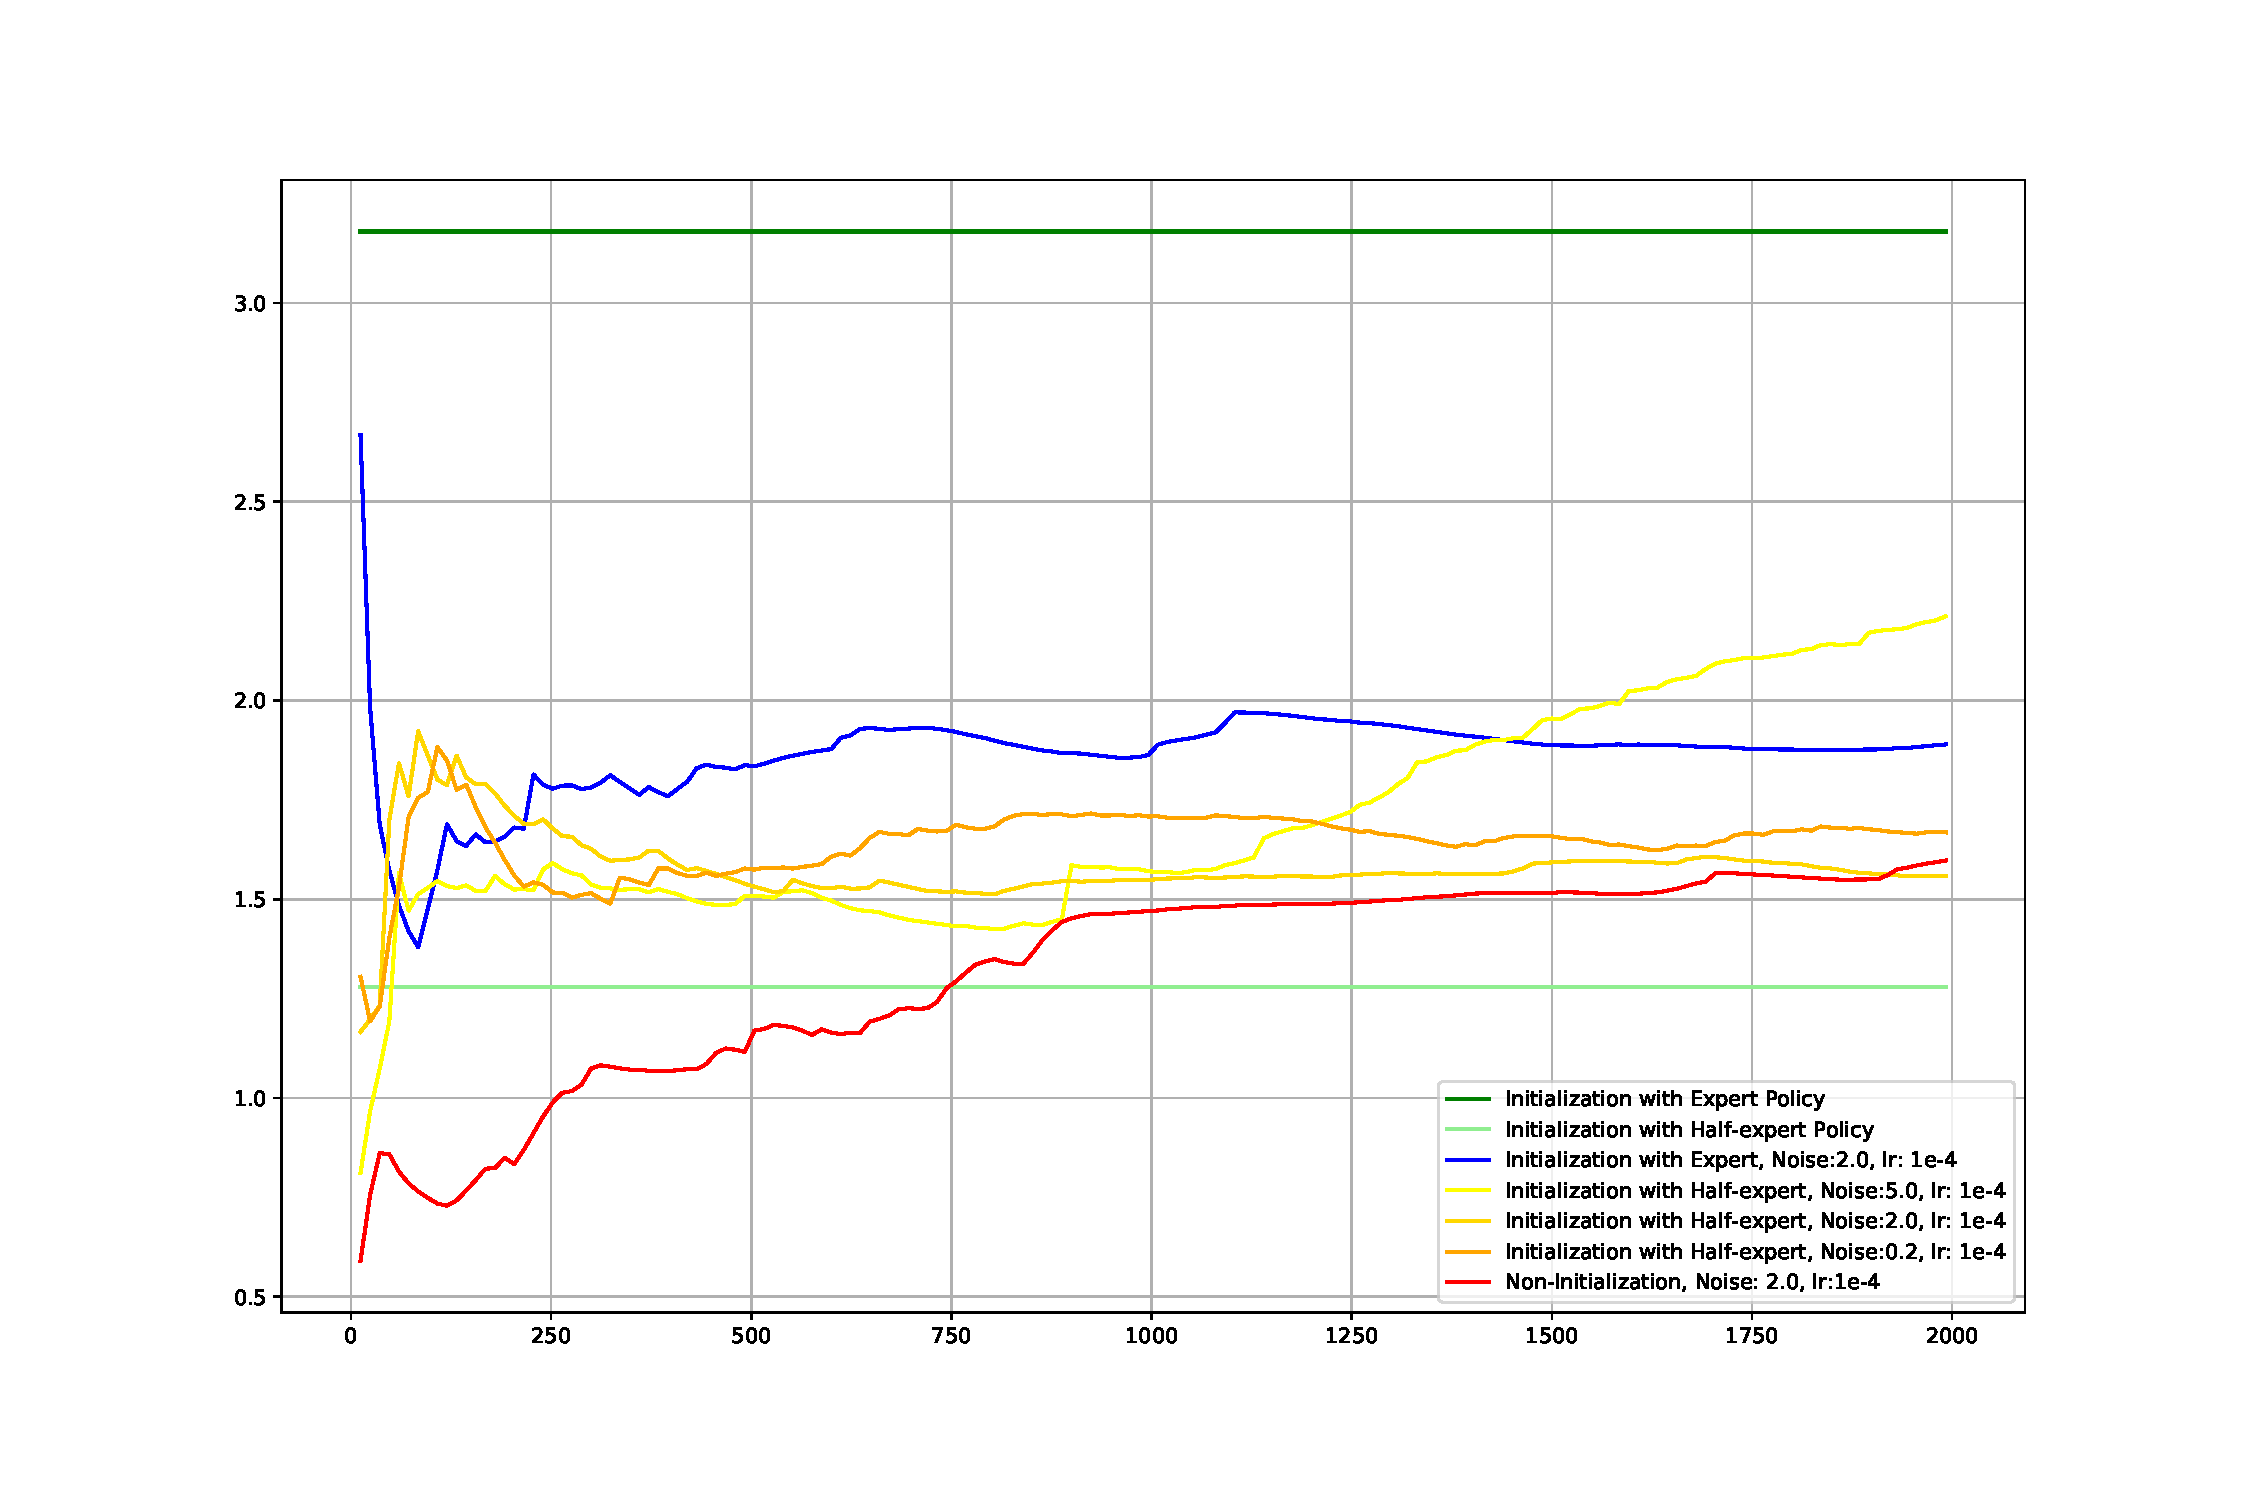
\includegraphics[height=260, width=450]{img/ddpg_compare3.pdf}
	\caption{Experiments with different initialized policy with different scale of exploration noise for DDPG on \textit{Reacher} task. Expert and half-expert are two initialization policies of different level of performance.}
	\label{fig:noise3}
\end{figure}

\begin{figure}[htbp]
	\centering
	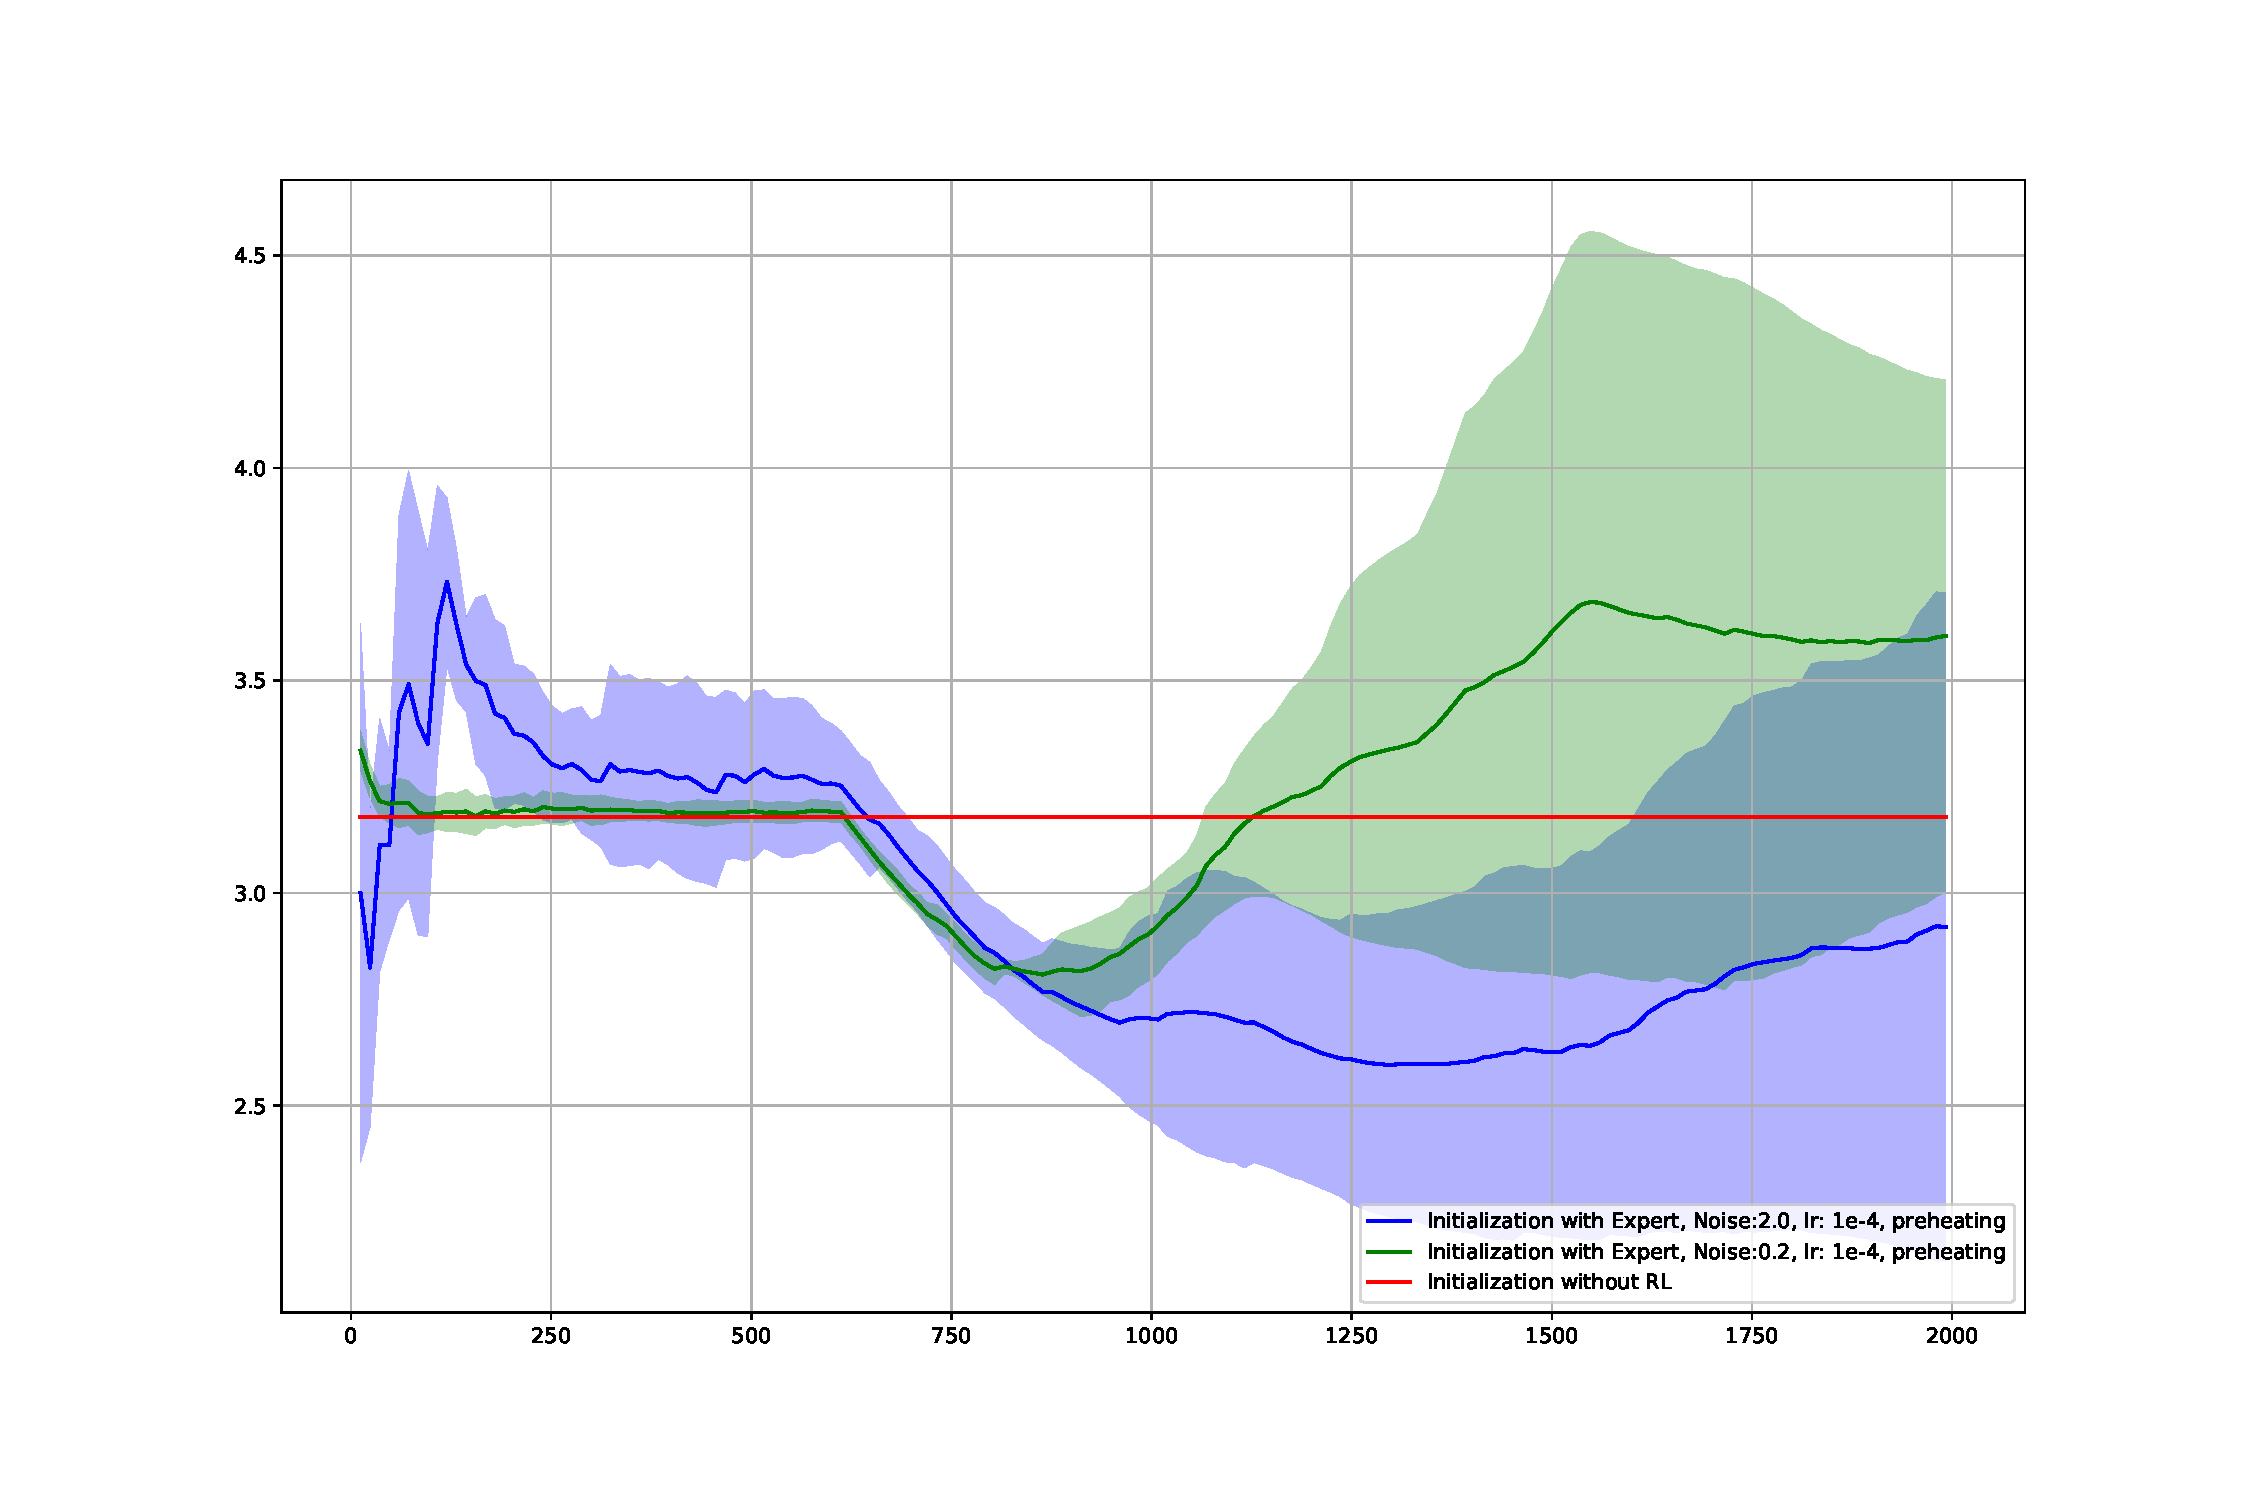
\includegraphics[height=260, width=450]{img/ddpg_compare4.pdf}
	\caption{Experiments with different initialized policy for DDPG on \textit{Reacher} task}
	\label{fig:noise4}
\end{figure}

\begin{figure}[htbp]
	\centering
	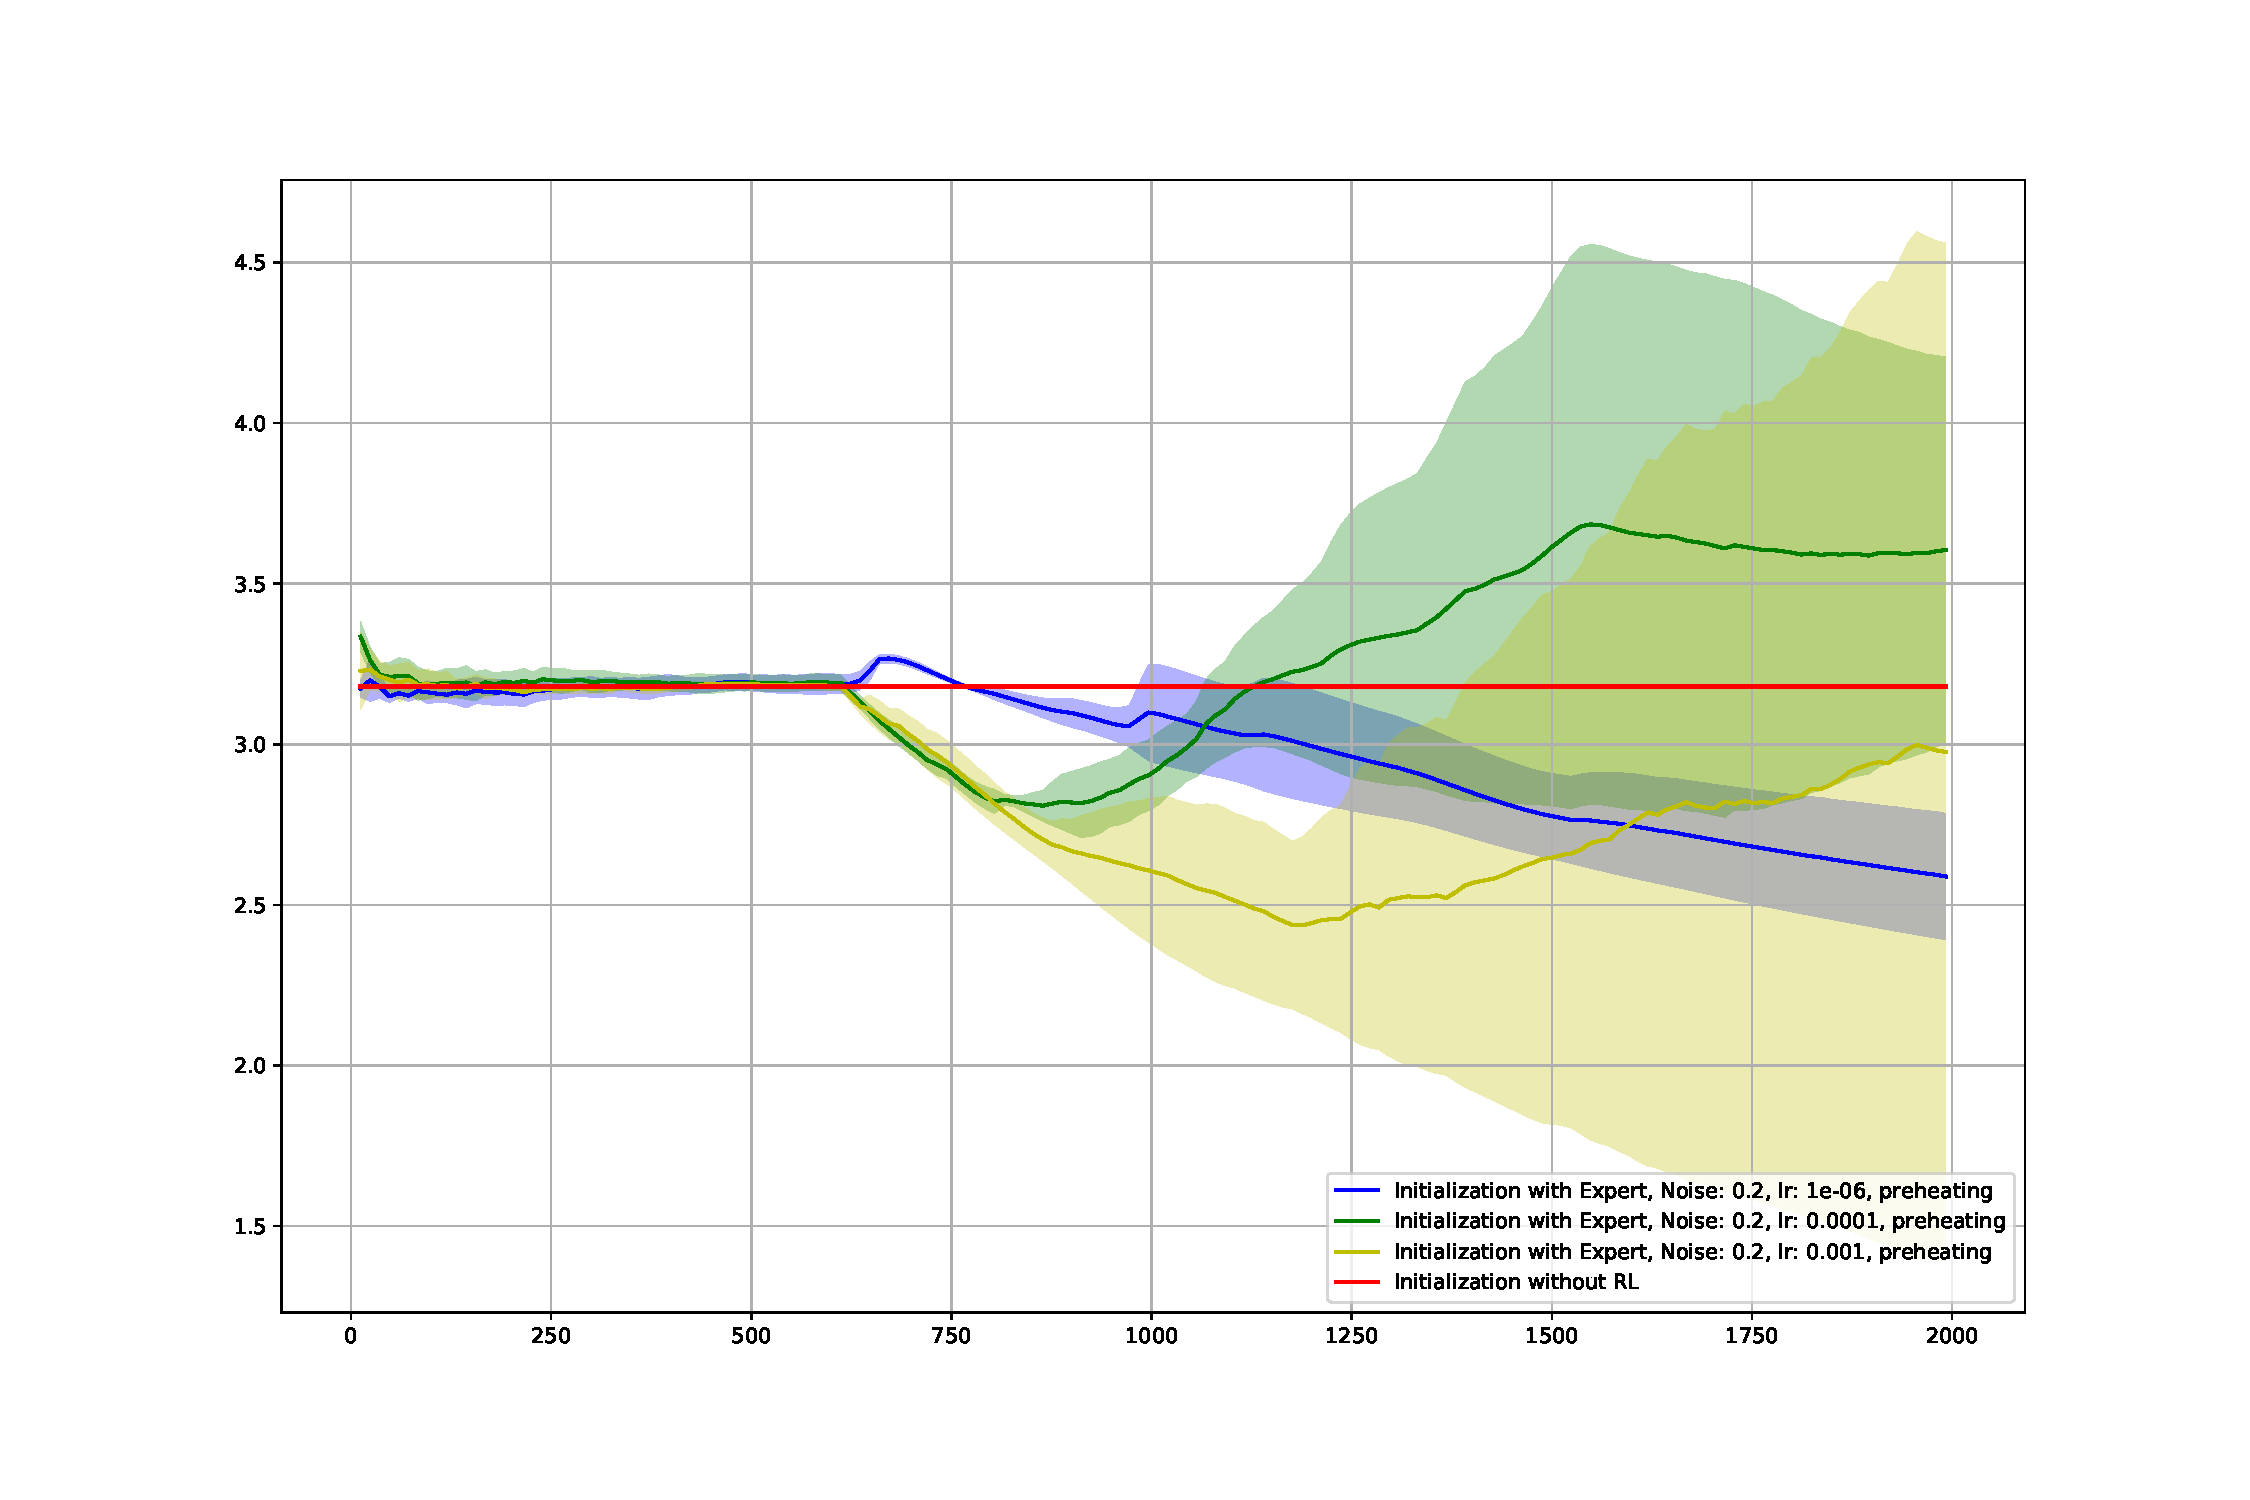
\includegraphics[height=260, width=450]{img/ddpg_compare5.pdf}
	\caption{Experiments with different initialized policy for DDPG on \textit{Reacher} task}
	\label{fig:noise5}
\end{figure}

As for the learning rate settings, Fig. \ref{fig:noise5} shows a comparison of different actor learning rate for initialized DDPG with a proper noise scale. For initialized DDPG from an expert policy, we actually need only to tune the parameters in the actor neural networks in a small range, which requires a small scale of actor learning rate (e.g. $10^{-4}$). A larger learning rate could change the networks dramatically and also the outputs. However, when the actor learning rate is too small, it will not help with learning process as shown in Fig. \ref{fig:noise5}.


\textbf{Pre-train the Critic}\label{pretrain}

The actor-critic scheme is important in DDPG, as the critic instructs the actor's choise of action values through evaluating the Q-value of each action. Therefore, a good critic is critical for the DDPG to show great learning performance in a task. However, in initialized policy for RL, the supervised learning with inverse kinematics could only mapping from the input states to the output actions, without any reference of the estimated value of each action. It means the critic of DDPG cannot be directly initialized with policy from supervised learning. Therefore, the role of the critic is amplified in the learning process of initialized DDPG, which is testified in experiments of this section. To solve the problem that the supervised learning policy can only initialized the actor networks, we propose a pre-training process of the critic in initialized DDPG called the 'preheating', with which the initialized policy could be more effective than without it.

The `preheating' process is conducted as follows: after loading the weights from pre-trained policy to the actor networks in DDPG, we sample from the frozen actor to generate near-expert samples with noise scale $\sigma$ and feed them into the memory (DDPG is off-policy learning), then train the critic networks with generated samples for $N_{pre}$ epochs. The frozen actor can be achieved through setting the actor learning rate to be 0 in practice. After the `preheating' step of $N_{pre}$ epochs, we train the initialized DDPG in a general way. 

As shown in Fig. \ref{fig:pretrain}, without pre-training the critic, there is always a severely decrease in performances of the initialized DDPG algorithm, no matter what the scale of exploration noise is. The decrease phenomenon for initialized DDPG without preheating can be explained as follows: the main problem of initialized policy for RL without preheating is that the virtue of initialized policy is ruined too quickly through changing of the weights of the initialized actor, and this is always the case as long as the learning rate is of a relatively considerable value. Because no matter how much the exploration noise is, the weights of the actor will be changed according to the learning rate of the actor, and neural network as an estimator has property of sensitivity on weights, which ends up with a dramatic changing in output policy of the actor. Therefore the actor will diverge fast from the initial near-expert policy, without a good critic. A good critic means it shows positive instructions for the actor to update weights in the correct direction. On the other hand, a good actor here in initialized DDPG will have great chances to decrease its performance with a random initialized critic. Therefore the `pre-heating' process actually prevent the actor from updating to hurt the performances, or at least alleviate it. This is shown clearly in Fig. \ref{fig:pretrain} that the lower bound of initialized DDPG with preheating is much higher than without the preheating process.
\begin{figure}[htbp]
	\centering
	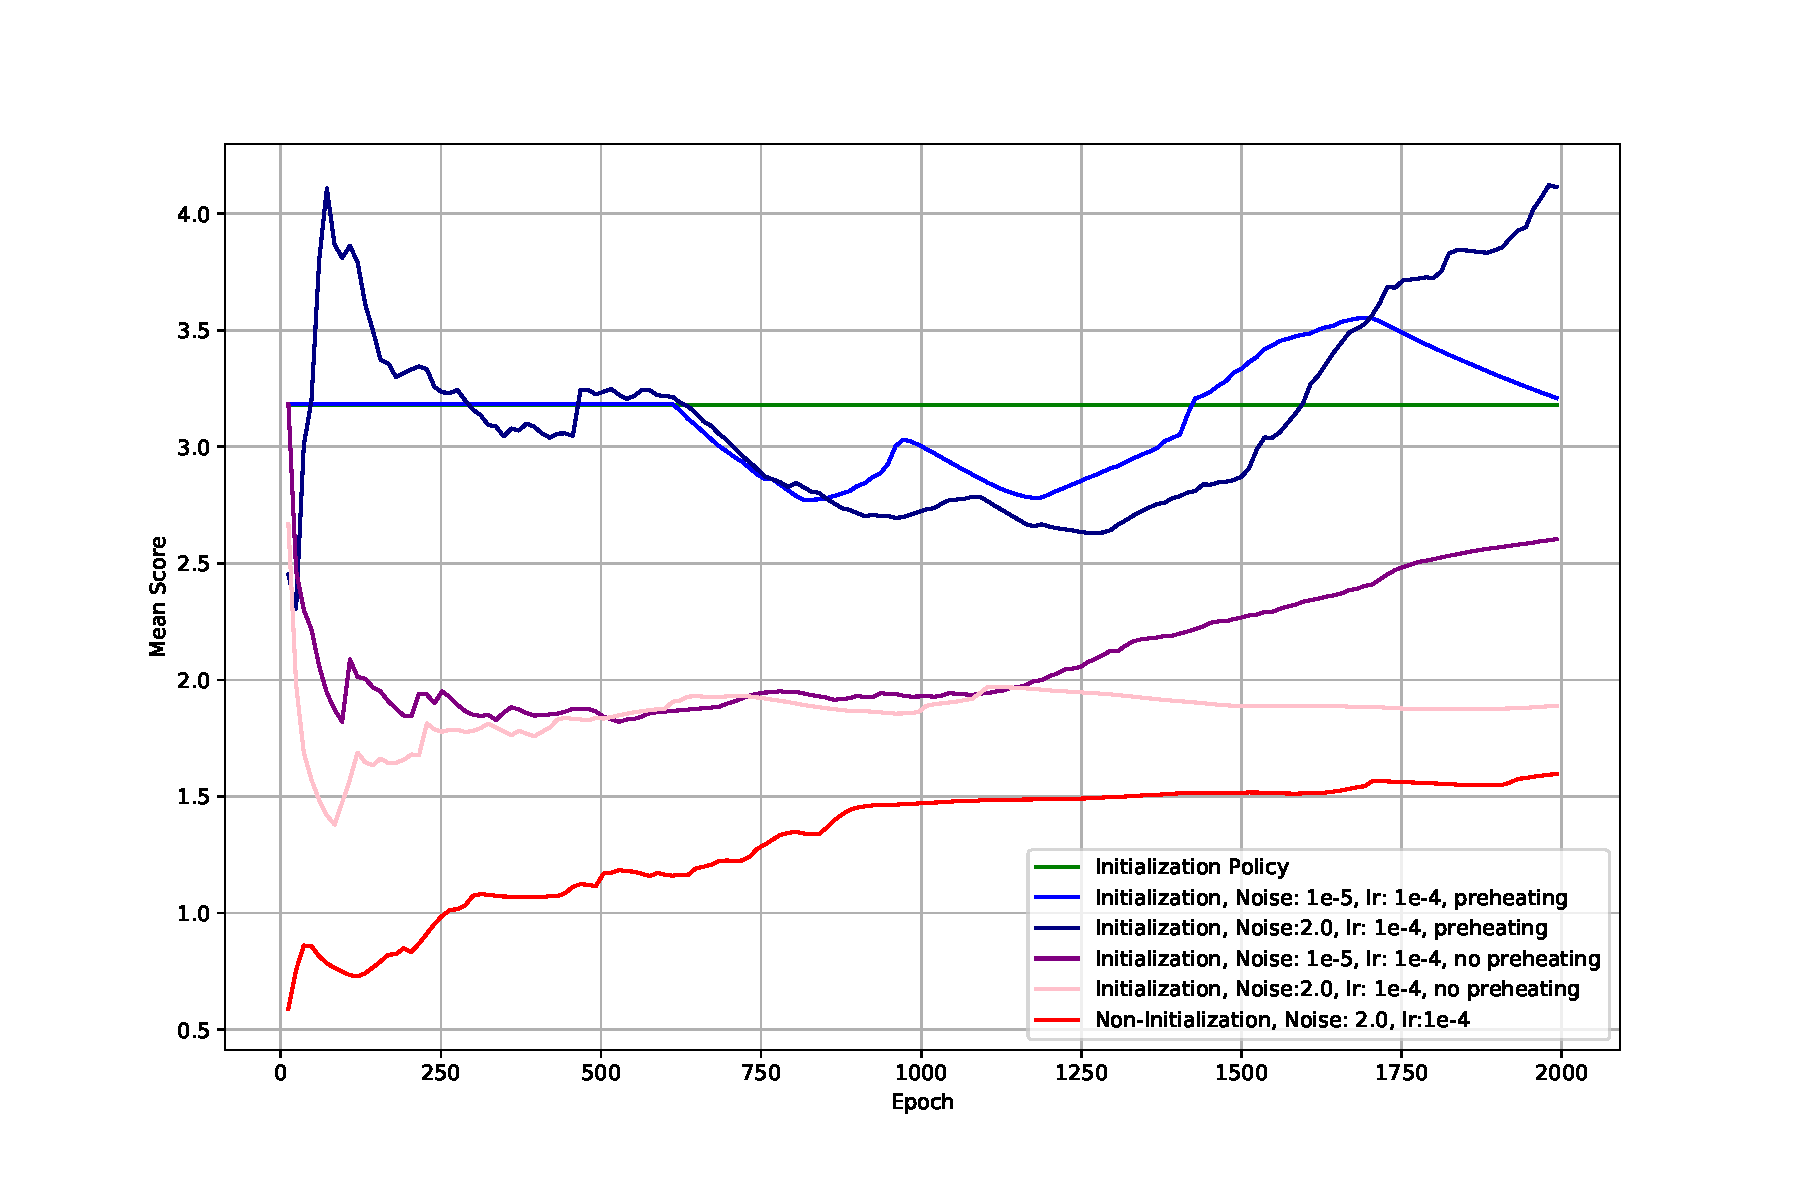
\includegraphics[height=260, width=450]{img/ddpg_compare2.pdf}
	\caption{Comparison of initialized DDPG with/without pre-training the critic on \textit{Reacher} task. The green line is the mean reward of initial policy trained with supervised learning.}
	\label{fig:pretrain}
\end{figure}

\textbf{Conclusions}

Some conclusions can be derived from above analysis and experiments about DDPG with initialization policy for \textit{Reacher} task:

(1). Different initial policy requires different noise scales to achieve better performances. For expert initialization policy, smaller exploration noise for DDPG shows better learning effects; for half-expert initialization policy, larger noise shows better learning effects.

(2). The preheating process is important for initialized policy on DDPG: with the pre-training of the critic before general learning process of DDPG, the learning performance is always better than without it, It reduces the dramatic decrease at the initial training phase when the DDPG is initialized with an expert policy. The important intuition from this is that we should not use the critic for instructing the actor unless it's good enough for a good actor.


\subsubsection{PPO with Policy Replacement}
PPO is an on-policy RL algorithm, and its exploration is controlled by the variance $\sigma$ of output action distribution from the policy neural network, which is learned during the training process. We can control the scale of exploration through adding a value to the variance, which is called noise base $\sigma_0$ here. So the actual action variance is $\sigma =\sigma_0+\sigma_{pre}$ where $\sigma_{pre}$ is trained output variance of the policy network.

The preheating process for PPO is conducted by pre-training the value evaluation network, similar to pre-training the actor in DDPG. 

Fig. \ref{fig:ppo1} shows comparisons of initialized PPO for \textit{Reacher} task. Similar to conclusions in initialized DDPG algorithm, the preheating process is effective for reducing the decrease in initial training phase of PPO when initialized from an expert policy.
\begin{figure}[htbp]
	\centering
	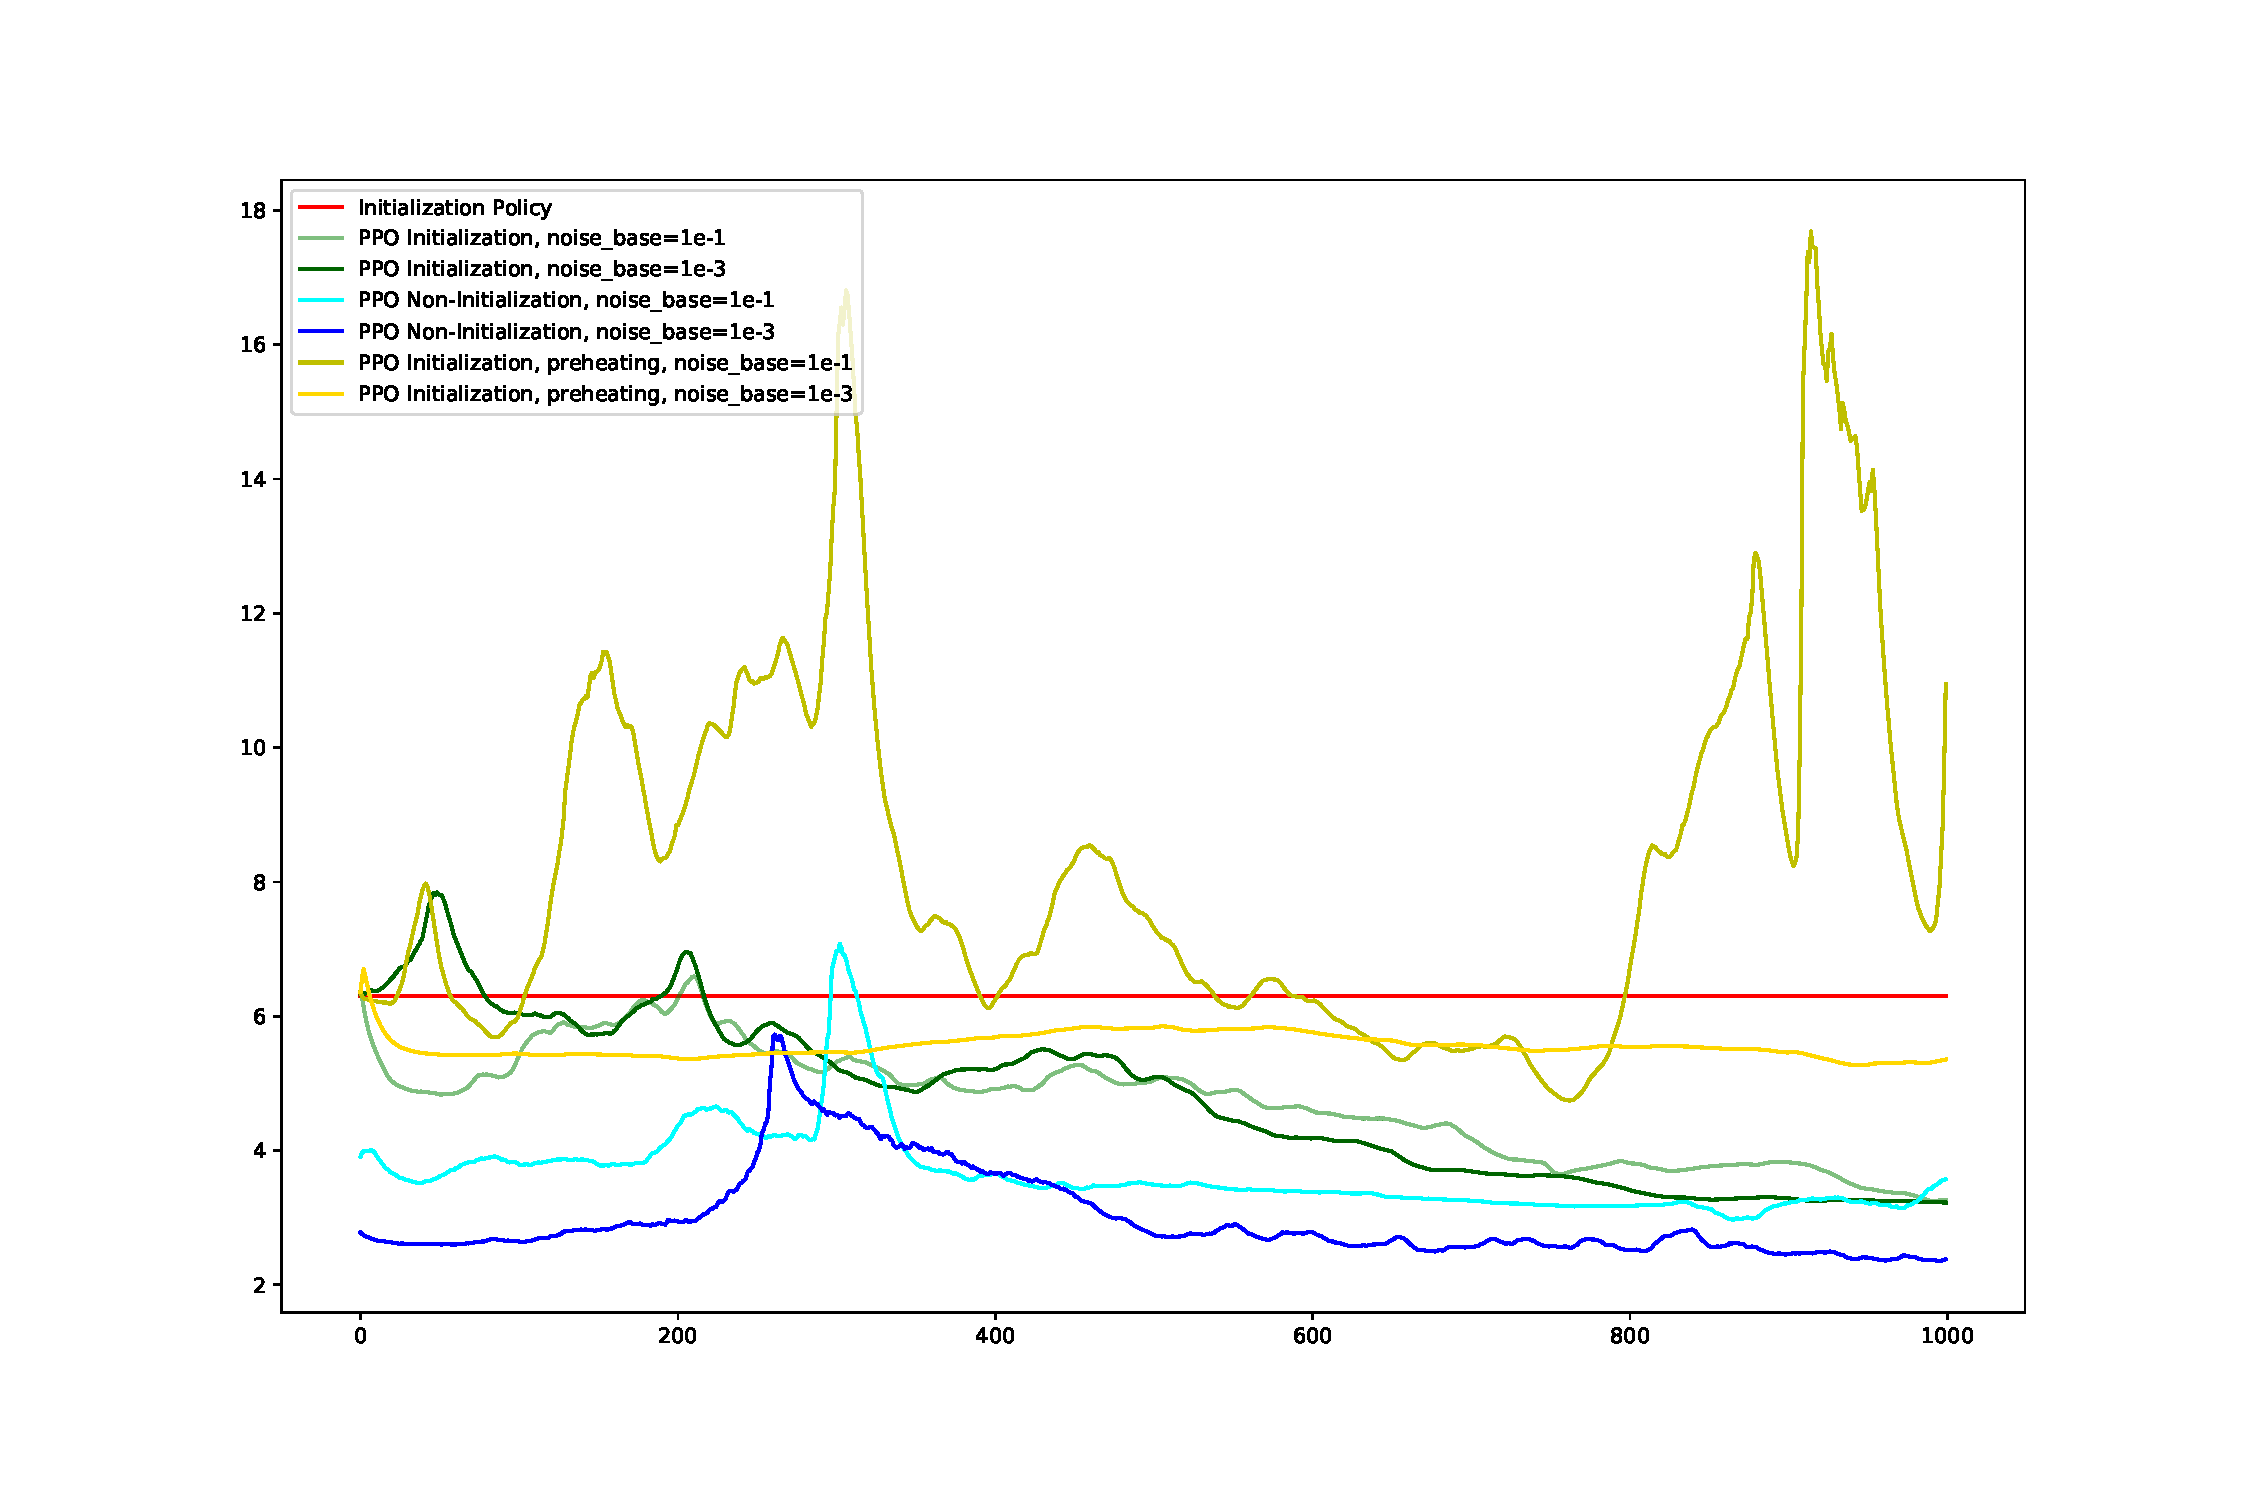
\includegraphics[height=260, width=450]{img/ppo_compare2.pdf}
	\caption{Comparisons of PPO with or without initialized policy and preheating process with different noise scale.}
	\label{fig:ppo1}
\end{figure}

\begin{figure}[htbp]
	\centering
	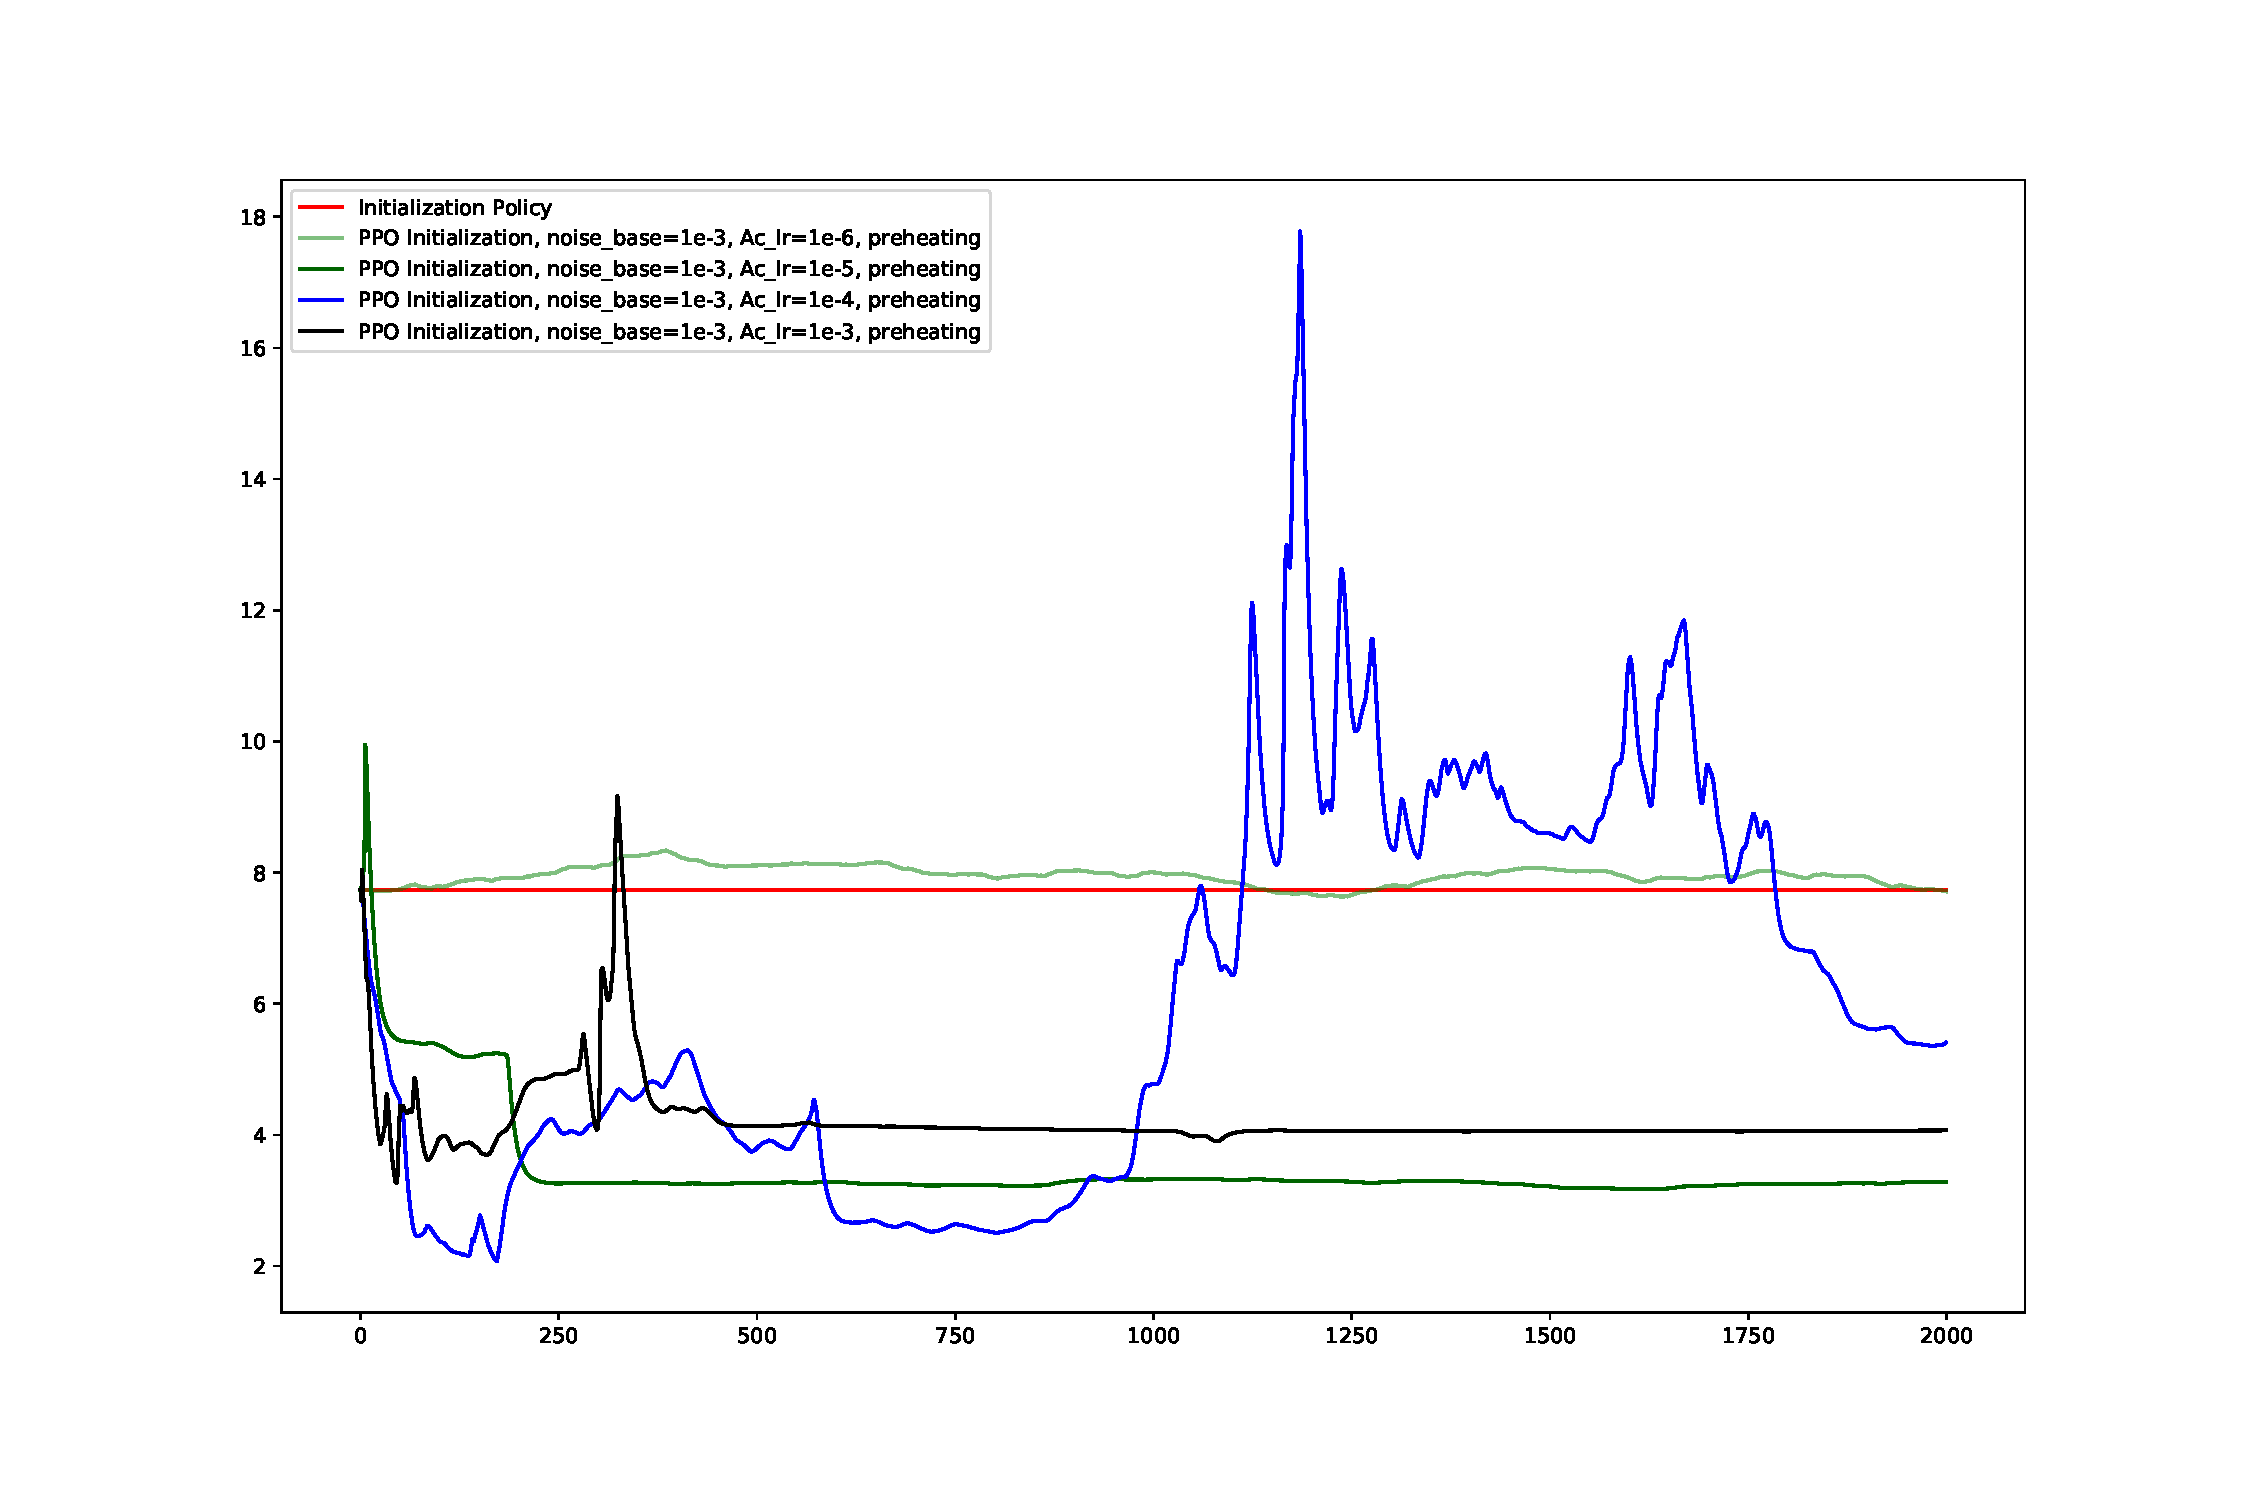
\includegraphics[height=260, width=450]{img/ppo_compare3.pdf}
	\caption{Comparison of different actor learning rates for initialized PPO with preheating process on \textit{Reacher} task.}
	\label{fig:ppo2}
\end{figure}

Fig. \ref{fig:ppo2} shows different actor learning rates for initialized PPO. A proper range of actor learning rate is needed for effective learning.

\begin{figure}[htbp]
	\centering
	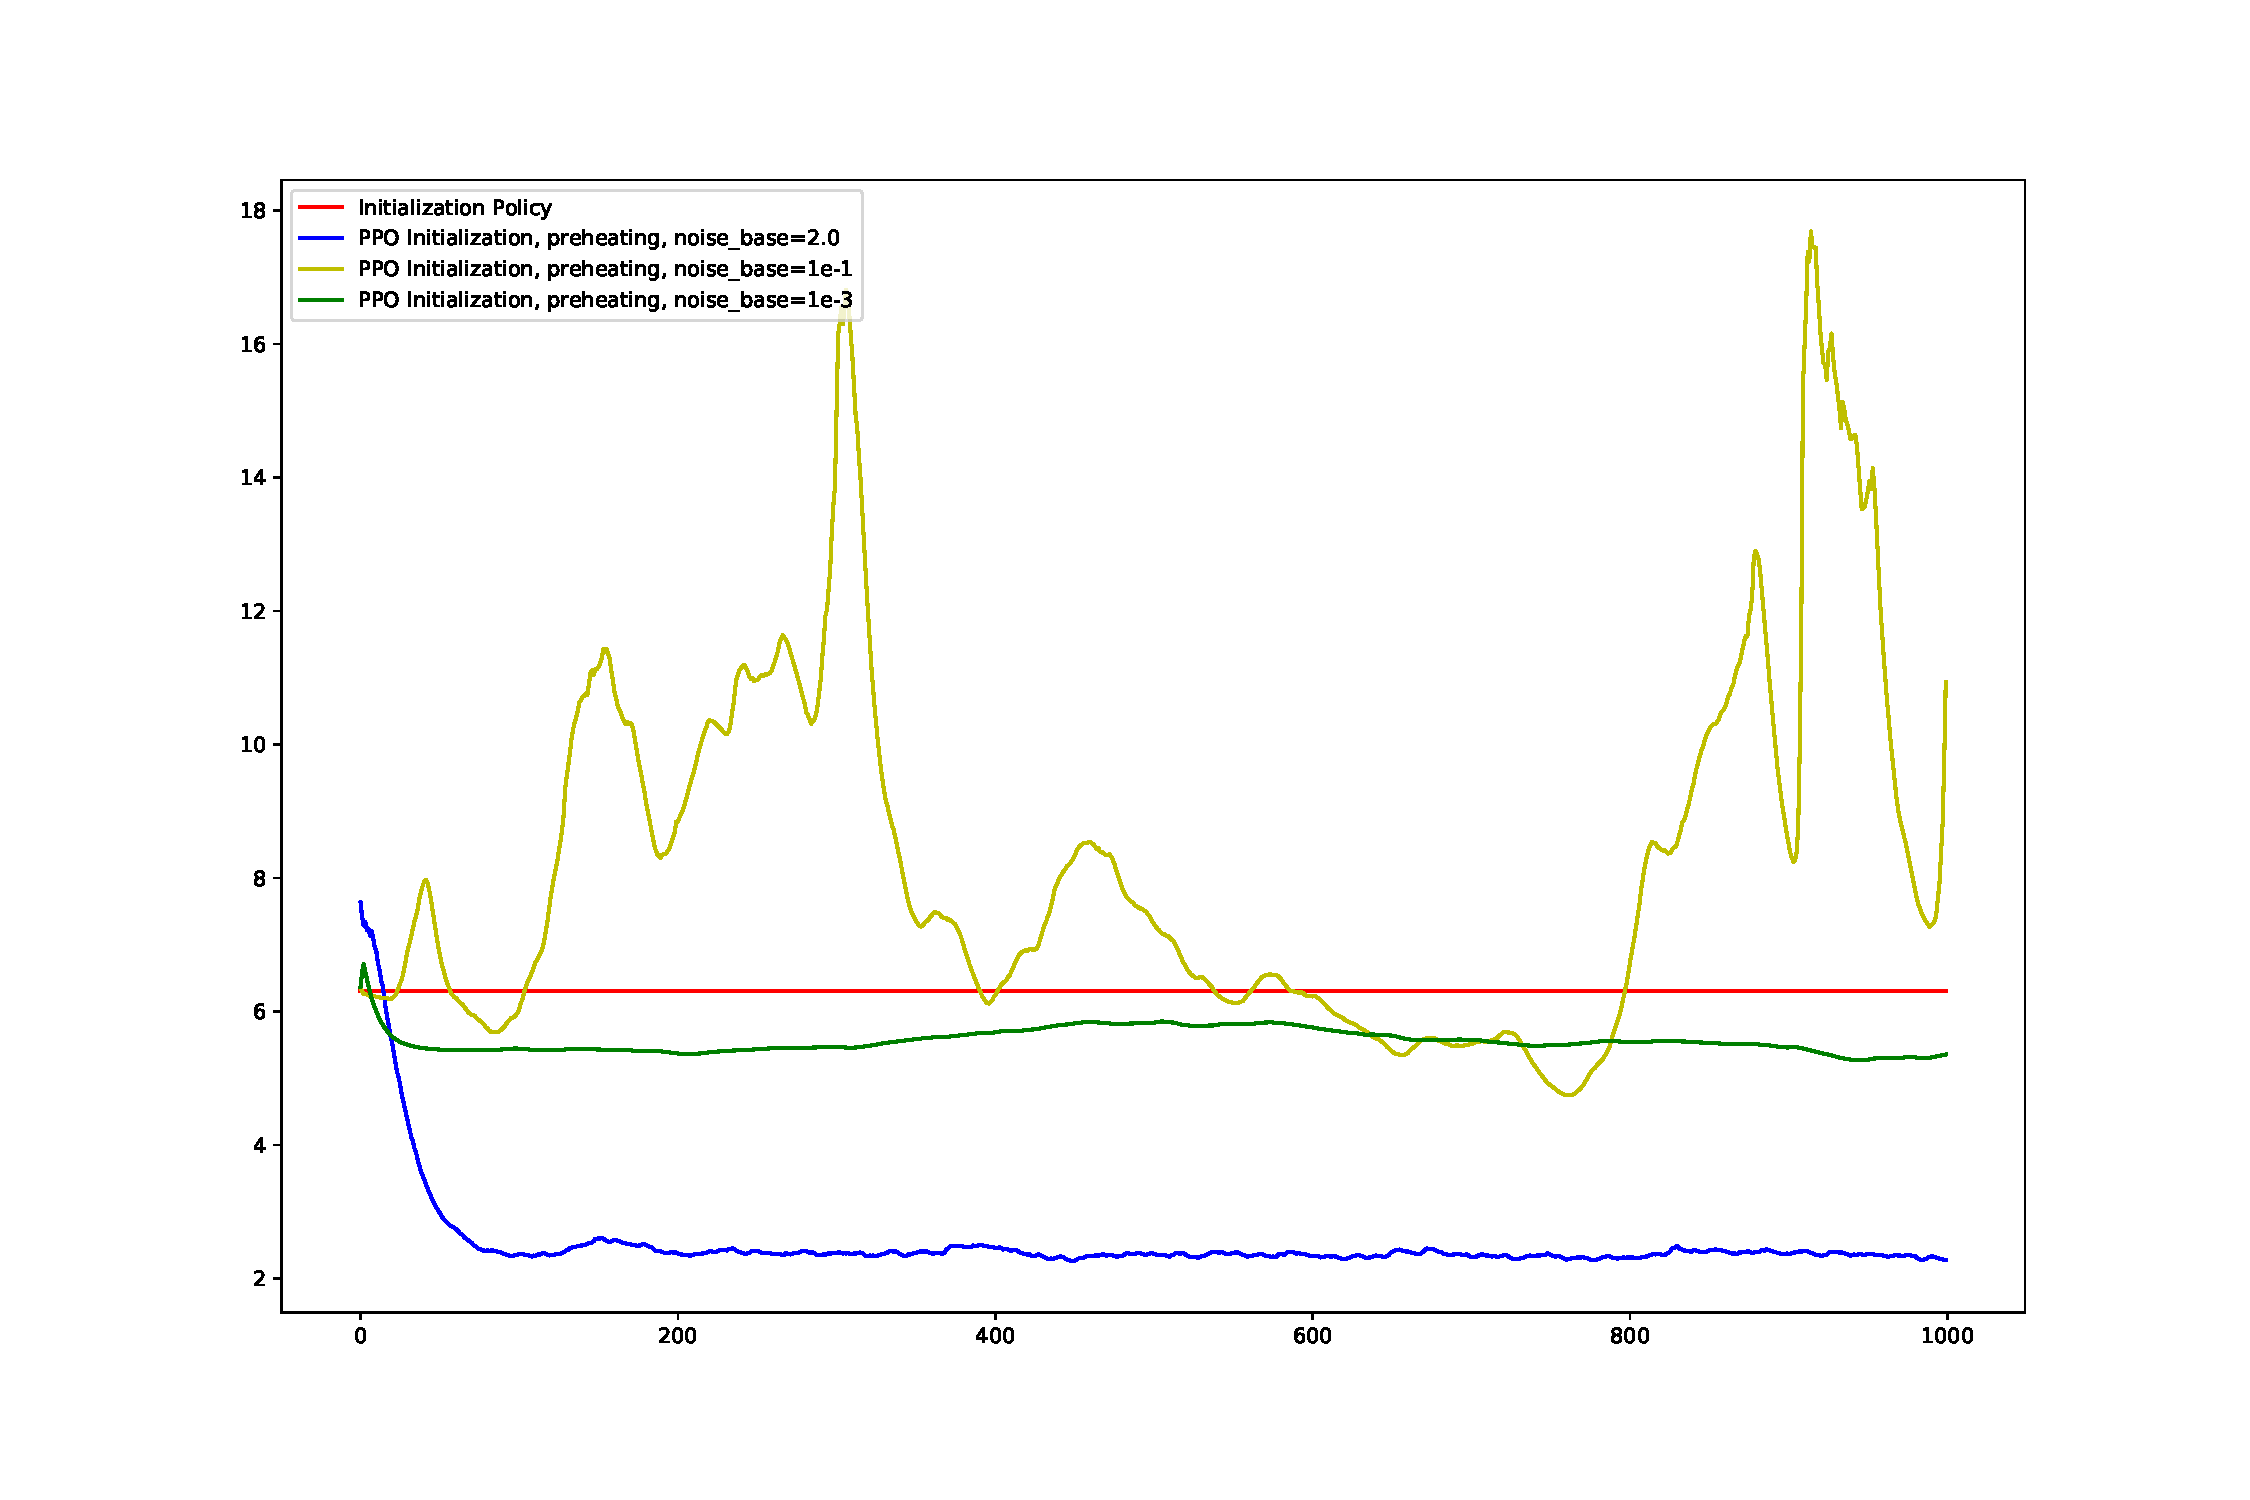
\includegraphics[height=260, width=450]{img/ppo_compare4.pdf}
	\caption{Comparison of different noise base for initialized PPO with preheating process on \textit{Reacher} task.}
	\label{fig:ppo3}
\end{figure}

Fig. \ref{fig:ppo3} shows different noise base for initialized PPO. A proper range of noise is needed for effective exploration and learning.

\subsubsection{Challenges of Policy Replacement}
In practice, policy replacement as a method of behaviour cloning in leveraging demonstrations for RL does not work very well, even with tricks like pre-heating process etc. The main challenges of this method lie in two aspects:

1. \textbf{Compounding error problem}: if we train a policy with a demonstration dataset as an initialization for RL, those states met in explorations of RL but not seen in the training dataset will drift the policy further away from the initialization policy trained on demonstrations, until the policy is able to make good decisions for those unseen states in the training dataset. And in policy replacement, the policy may be drifted rapidly in the RL process and make it not able to perform well in those seen states in demonstrations. This process can be regarded as a generalization process from the initialization policy to a more general policy for the task.

2. \textbf{Difference in training objectives}: as we know, the training objective in imitation learning to train the initialization policy is of the form Eq.(\ref{equ:bc}). However, when we initialize the RL with this pre-trained initialization policy, take DDPG as an example, the loss function of the actor network is to maximize the action value $Q(s,a)$ of its predicted action $a$ with the input state $s$, and it is back-propagated from the critic network. The difference in training objectives in supervised imitation learning and RL algorithms will cause a discrepancy in the direction of optimization, which is another source of wasting of computation in training. Therefore, \textbf{it may have better performance if the training objective of supervised imitation learning could be implemented in the same form as the RL training does}. Some methods are proposed to achieve that.

\subsection{Initialized Reinforcement Learning with Supervised Learning Policy -- Residual Policy Learning}
In addition to the policy replacement approach for initialization of RL, residual policy learning \cite{johannink2018residual} is another approach to realize initialization. It s based on good but imperfect controllers for robot manipulation tasks, and to learn a residual policy on top of that initial controller. For robot manipulation in real world, the initial controller could be a pre-trained policy in simulation; and for robot manipulation in simulation, the initial controller could be from the pre-trained supervised learning with expert trajectories as in Section 3.2.

The action in residual policy learning is the sum of the initial policy $\pi_{ini}$ and the residual policy $\pi_{res}$:
\begin{equation}
a=\pi_{ini}(s)+\pi_{res}(s)
\end{equation}
In this way, the residual policy learning is able to preserve the initialized policy performance to the best advantage. Some tricks are applied to guarantee that: 

(1). The weights of the output layer of the actor in RL are initialized to be 0;
 
(2). The same preheating process as in DDPG with initialization using policy replacement approach: train the critic while fix the weights of the actor to alleviate the decrease in initial RL training stage caused by a bad critic;

(3). Apply amplification factor for noise scale during the preheating process: for pre-training the critic to have better generalization ability, apply noise multiplied by an amplification factor in the preheating process and reduce it to normal when training the actor.

Note that with above settings, the actor network outputs are actually all 0 during the preheating process, so the action values are fully attributed to the amplified noise and initial policy, which means $\pi_{res}=\epsilon$ and also:
\begin{equation}
a=\pi_{ini}(s)+\alpha * \epsilon, \alpha>1
\end{equation}
where $\epsilon$ denotes the action noise and the $\alpha$ denotes the amplification factor. And the action values stored in the memory (with DDPG algorithm) are $\pi_{res}=\epsilon$ during preheating. This is not a problem as we only train the residual policy $\pi_{res}$ instead of the composite policy $\pi_{ini}+\pi_{res}$, and action values stored in memory are just $\pi_{res}(s)$ instead of the real action value $a$. Correspondingly, the estimated Q-values learned by the critic are also only for the residual policy, which are $Q(s, \pi_{res}(s)))$.

However, there are still several freedoms to be set in residual policy learning, e.g. the scale of the output action from the residual policy can be chosen arbitrarily, which is actually a trade-off between the initialized policy and the learning policy, etc.

\subsubsection{DDPG with Residual Policy Learning}
We experimentally apply the DDPG algorithm for leveraging the demonstrations with residual policy learning. According to the residual learning, the actor policy in DDPG consists two parts: one is the pre-trained initialization policy, which will be fixed after initialization; and another one is the residual policy to be trained during the learning process. The initialization policy is pre-trained with the demonstration samples generated from inverse kinematics, which is the same as the policy replacement method. The pre-trained initialization policy only works for the actor part in DDPG. The process of applying residual policy learning in DDPG is as follows:

(1). Initialize all neural networks in DDPG with residual learning, including a general initialization of the critic, target critic, and an initialization with zero-value final layers for the residual policy and the target residual policy, and a policy replacement for the initial policy and the corresponding target, totally 6 networks. Fix the initialized policy and its target, and start the training process.

(2). Let the agent interact with the environment, and the action value is the sum of the action values from the initialization policy and the residual policy: $a=a_{ini}+a_{res}$; store samples in the form of $(s,a_{res}, s', r, done)$.

(3). Draw samples $(s,a_{res}, s', r, done)$ from the memory buffer, we have:
\begin{equation}
    Q_{target}(s,a_{res})=r+\gamma Q^{\mathcal{T}}(s, A_{res}^{\mathcal{T}}(s))
\end{equation}
where $Q^{\mathcal{T}}, A_{res}^{\mathcal{T}}$ denote that the values are calculated with the target networks, the target critic and the target residual actor policy respectively. The critic loss is MSE$(Q_{target}(s,a_{res}), Q(s,a_{res}))$. And the objective for the actor is to maximize the action-value function of state $s$ and action $a_{res}$ as follows:
\begin{equation}
\maximize Q(s,a_{res})=Q(s,A_{res}(s))
\end{equation}

(4). Repeat above steps (2)(3) until the policy is converged.

Compared with general DDPG algorithm, the difference of applying residual policy learning is just to learn action-value function and the policy with respect to the residual policy actions instead of the overall action values for the agent.

\subsubsection{Comparison of Residual Learning and Policy Replacement}
We chose the goal position to be easy enough to reach for the agent, in order to shorten the training process and show the overall learning curves, like the left one in Fig. \ref{fig:rpl1}.
\begin{figure}[htbp]
	\centering
	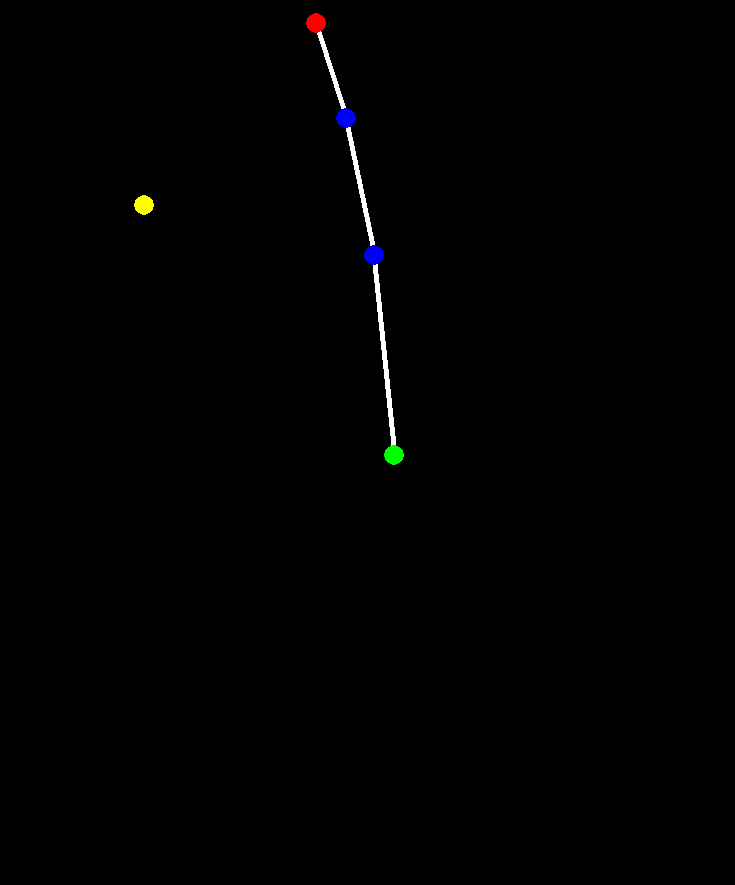
\includegraphics[width=150, height=200]{img/goal_position.png}
	\hspace{1cm}
	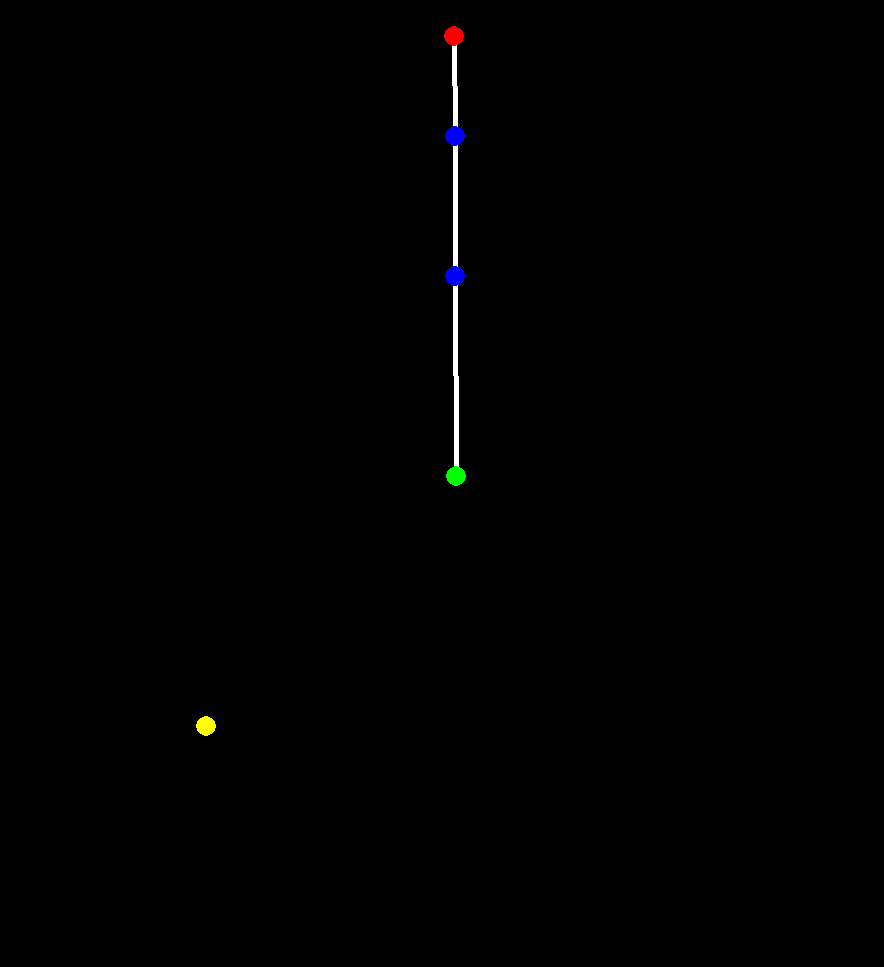
\includegraphics[width=150, height=200]{img/goal_position1.png}
	\caption{Different goal positions (the yellow dot) for \textit{Reacher}. The left one is easier to reach than the right one with vertical initialization for \textit{Reacher}. It will affect the difficulty for the agent to reach the goal.}
	\label{fig:rpl1}
\end{figure}

With the same experiment settings: actor learning rate = 1e-4, critic learning rate = 1e-4, steps per episode = 12, same actor and critic network structures, preheating steps = 600 in initialized RL, noise scale = 2.0. The comparisons of non-initialized policy and initialized policy with residual Learning and policy replacement on DDPG for a easy-to-reach goal are shown in Fig. \ref{fig:rpl2}. For some easy-to-reach goals, the policy replacement approach seems to outperform the residual policy learning and non-initialization RL.
\begin{figure}[htbp]
	\centering
	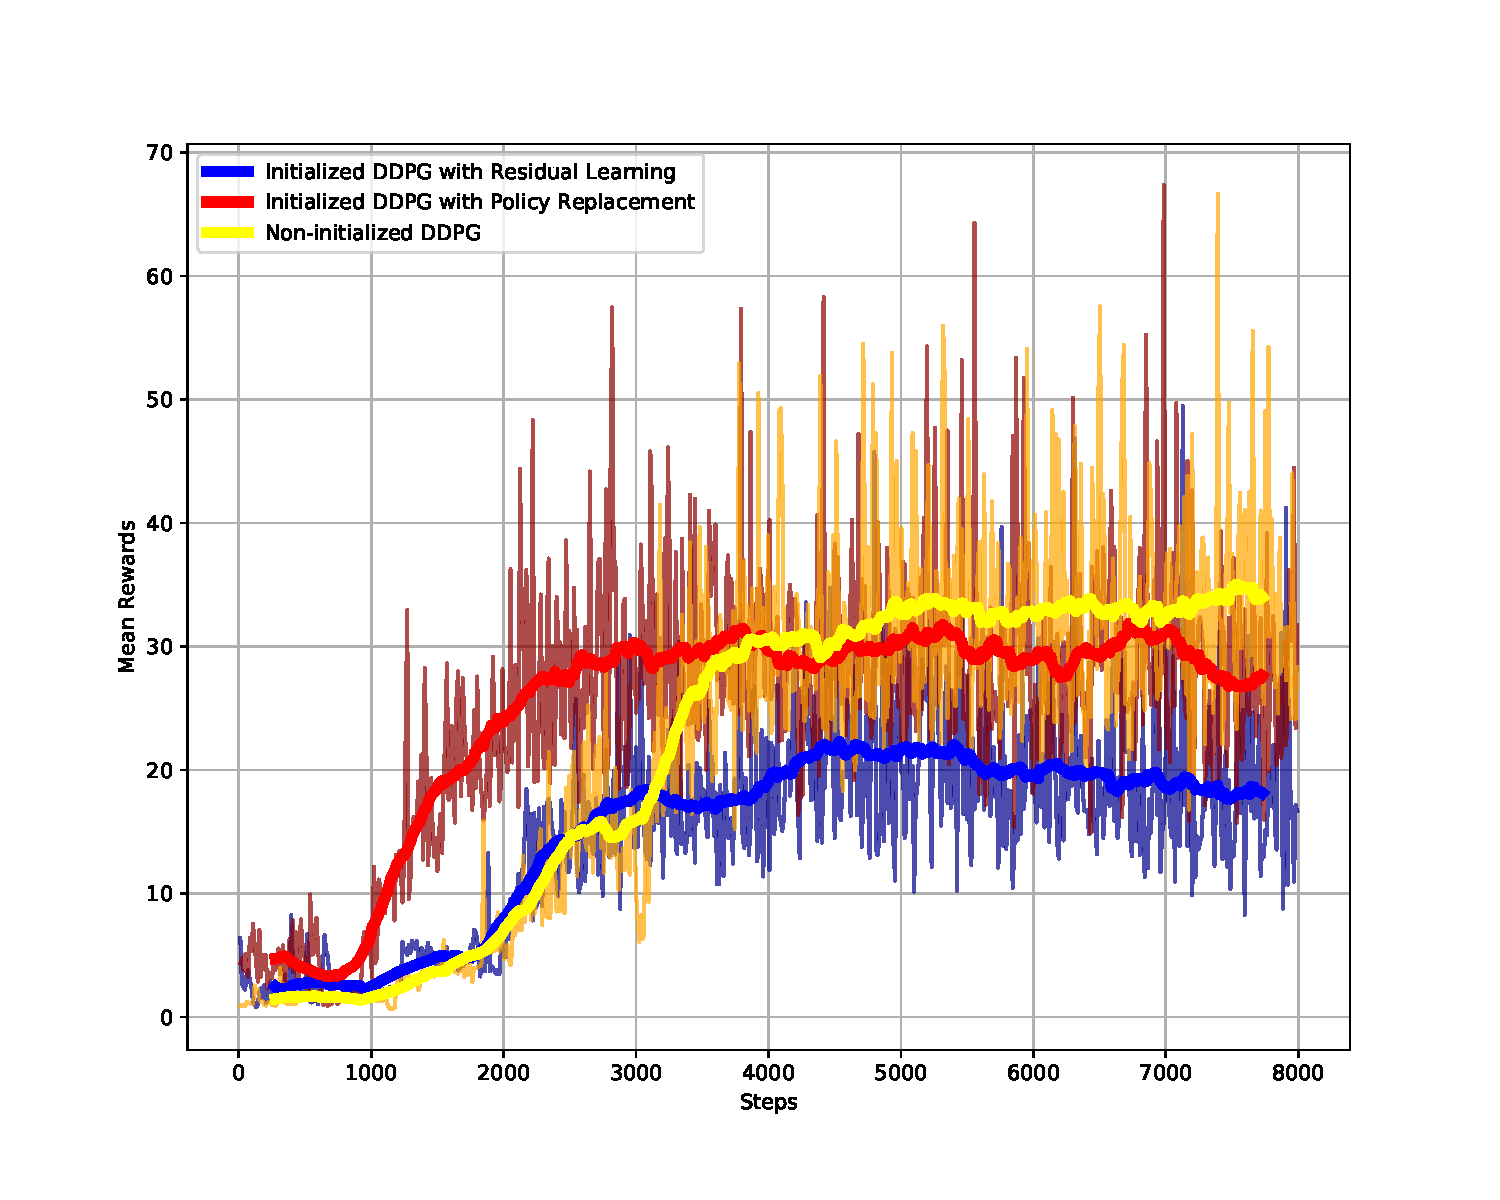
\includegraphics[height=250, width=400]{img/res_ddpg3.pdf}
	\caption{Comparison of non-initialized policy and initialized policy with residual learning and policy replacement for DDPG with an easy-to-reach goal position. The bold lines are moving average of episode rewards during learning process. The initialized policy has a preheating process of 600 steps.}
	\label{fig:rpl2}
\end{figure}

Comparison in Fig. \ref{fig:rpl3} shows that, for some other goals, initialization with residual learning may not learn as well as policy replacement at the beginning of training, but will eventually learn better policy. This may benefit from the performance guarantee of the initial good policy for residual policy learning, while in policy replacement the learning process may search in a larger trajectories space (testified in observing the experiments). 
\begin{figure}[htbp]
	\centering
	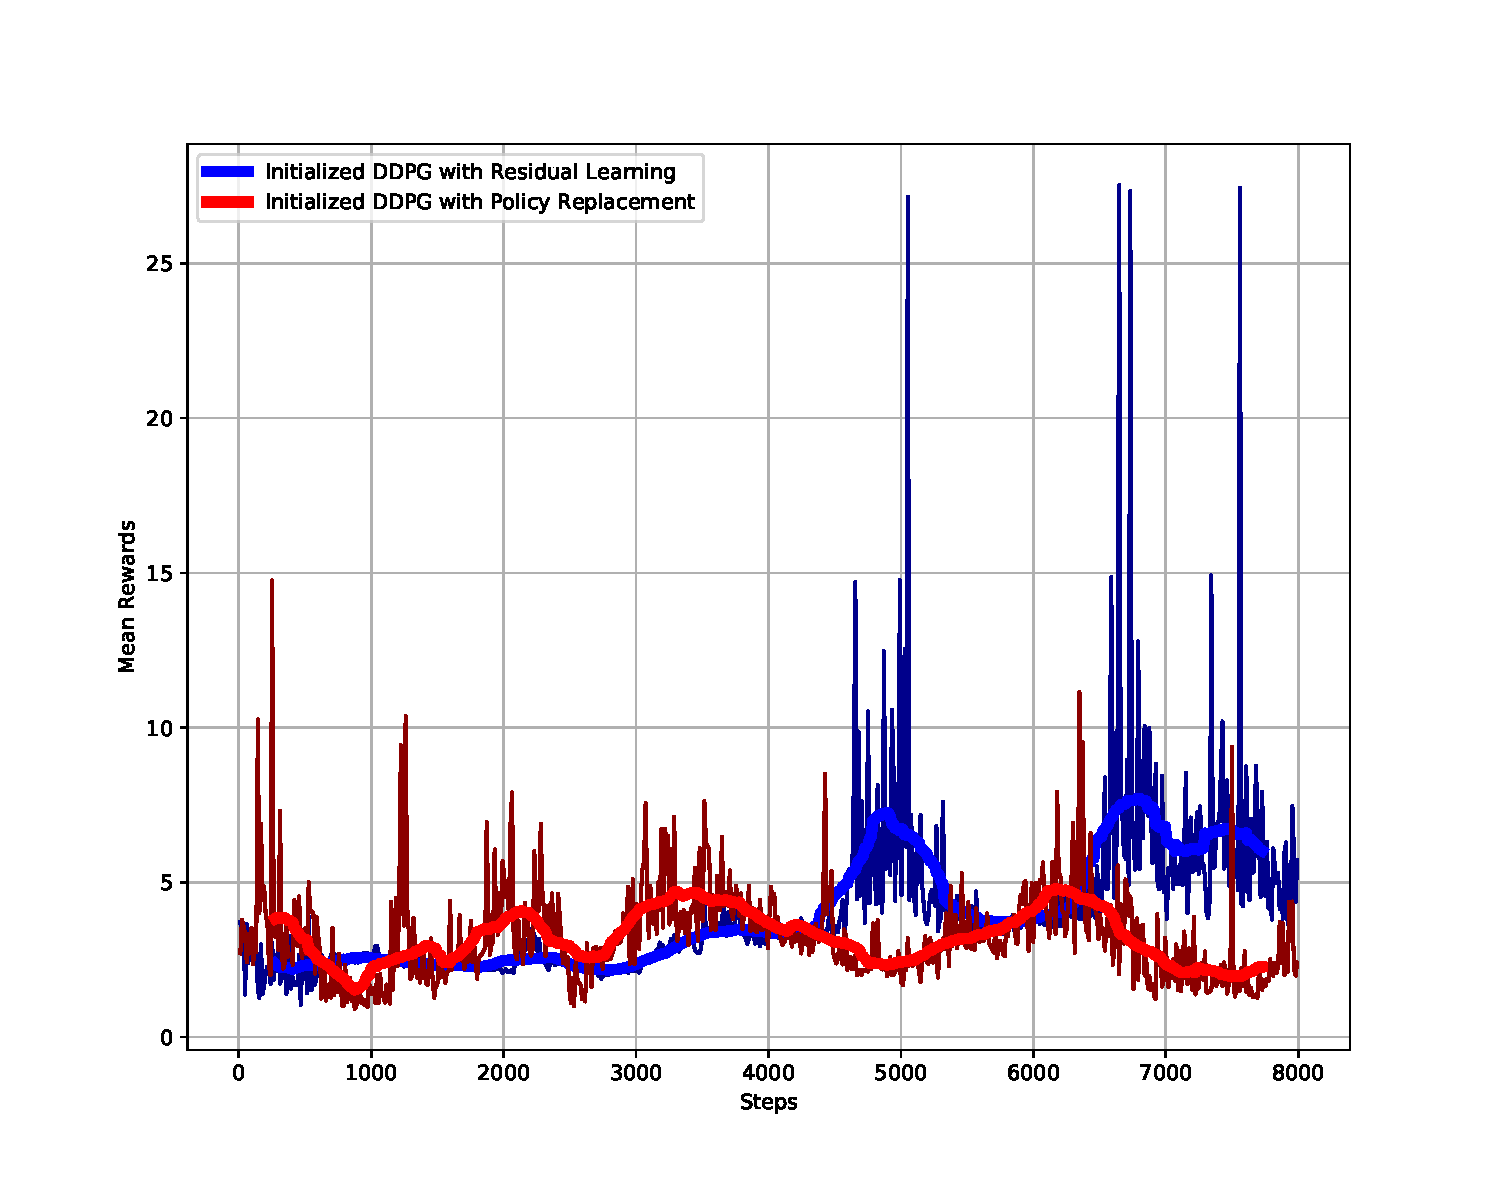
\includegraphics[height=250, width=400]{img/res_ddpg2.pdf}
	\caption{Comparison of residual learning and policy replacement for DDPG with another goal position (the one on the right in Fig. \ref{fig:rpl1}).}
	\label{fig:rpl3}
\end{figure}

With above analysis, we can see that the performances of different approaches to initialize the RL actually have large variance, which are significantly affected by parameters settings and task specifications like goal position, etc. 

\subsubsection{Modelling Analysis of Residual Policy Learning}
Consider that the residual policy learning is actually using policy $\pi_{res}(s)$ to generate the residual action, whose inputs $s$ are exactly the same as the initial policy $\pi_{ini}(s)$, the modelling of residual policy is actually may be more complicated than a general policy in RL, although the value range of outputs for residual policy may be smaller (a smaller searching space for delicate actions). In order to have a more accurate composite action, the residual policy not only needs to model the environment but also the initial policy. The modelling relationship can be interpreted as follows. 

We denote the modelling of a general policy in RL as $\mathcal{M}_g$, the modellings of the initial policy and the residual policy are $\mathcal{M}_i, \mathcal{M}_r$, respectively. A modelling means a mechanism that the policy learned from interactions with its environment to represent the its environment and based on which the policy determines actions. The relationship of above modellings is:
\begin{equation}
	\mathcal{M}_g = \mathcal{M}_i \oplus \mathcal{M}_r
 \end{equation}
 which means the $\mathcal{M}_i, \mathcal{M}_r$ are actually dual modellings with respect to a $\mathcal{M}_g$. As we only train the residual policy in the learning process of residual RL, we have the modelling to construct in this training process the $\mathcal{M}_r$:
 \begin{equation}
 \mathcal{M}_r = \mathcal{M}_g \ominus \mathcal{M}_i
 \end{equation}
 where the $\oplus, \ominus$ denotes a positive or negative modelling composite relationship. And the composite relationship does not determine the complexity of the composite modelling to be more or less than original constituent modellings, which means the modelling of $\mathcal{M}_r$ may not be less complicated than the general policy $\mathcal{M}_g$, and sometimes even more complicated than $\mathcal{M}_g$. This means the learning of a residual does not have to be easier than directly learning the general policy, if the range of the action value for the residual policy is not smaller than a single policy. But with two key components, we can make residual policy easier to learn than learning from scratch: \textbf{(1). a good initialization policy; (2). a small range of action value for the residual policy}, as discussed in the following.

\textbf{Discussions}

In practice, take the example of using neural networks as approximators for the initialization policy (like an expert controller) and the residual policy, we can actually manually choose the complexity of the networks and range of the outputs of each of them, which can be induced by some human knowledge prior or preference. The knowledge prior can be understood as that if we know that our initialization policy is good enough, then we can restrict the output range of the residual policy as an additional action to be small; and the preference can be understood as that if we require the robotics trained in physical world to move within a safe range \cite{chow2014algorithms}, we can also achieve it through restricting the output range of the residual policy. In this case, the residual policy learning with a smaller range of action value will have larger chances to reach a higher reward, if the initialized policy is a good one. And therefore it could be easier for the policy to be trained well than a single policy from scratch. \textbf{The residual policy learning enables us to apply some extra tricks (restrictions, bias, preferences, etc) on the residual policy without affecting the initial policy, to improve the learning performance overall.}

However, it may not works sometimes with restrictions on output range of the residual policy, especially when we apply an activation function like tanh or sigmoid and the optimal output values may fall out of the range of the output values we restrict the residual policy to have. It will cause the neural saturation in the output layer and vanishing gradients, and therefore slow down the learning process greatly or even stop the improvement. And if we don't restrict the output of the residual policy, the large variance of its exploration will have chances to overwhelm the initial policy. And according to above analysis, the learning of residual policy does not have to be simpler than the overall actor policy with the same range of action value, therefore learning a residual aside from a good initialization policy may not show advantages over learning the actor policy without fine-tuning on range of action value for the residual policy.

\subsection{Off-Policy Reinforcement Learning with Demonstrations Fed into Memory Buffer}
We show different initialization strategies for efficient RL as above, and leveraging demonstrations for deep RL is an alternative approach to learn efficiently. Both initialization approach and leveraging demonstrations approach are taking advantages of the expert trajectories, however, they treat them differently. Instead of pre-training a policy to initialize the RL policy, the approach of leveraging demonstrations directly feeds those expert trajectories into memory of off-policy RL (e.g. DDPG), to train the policy with both demonstrations and explorations. We show some experiments about the method of DDPG from demonstrations (DDPGfD) \cite{vevcerik2017leveraging}, without using the technique of prioritized experience replay \cite{schaul2015prioritized}.

We apply a more complicated environment for this experiment as shown in Fig. \ref{fig:ddpgfd0}, with two penalty areas. The optimal trajectories for the agent is to go through the middle of two penalty areas. And we generate good demonstrations by manually setting an intermediate goal position at the middle of two penalty areas.

Experiment results of the DDPG from demonstrations approach for efficient RL with different ratios of demonstration data over all training data are shown in Fig. \ref{fig:ddpgfd2}. The demonstration data contains 50 episodes of trajectories in the above $\textit{Reacher}$ environment with obstacles, with 21 steps for each episode. Aside from a general memory for storing exploration data in off-policy DDPG, there is an additional demonstration buffer for storing the data from expert-demonstrations at the beginning of the training. The ratio of demonstration data is used for balancing the data sampled from demonstration buffer or from the exploration memory for each training step. From Fig. \ref{fig:ddpgfd2}, the learning performance of DDPG algorithm trained without demonstration data (ratio of 0.0) or totally from the demonstration data (ratio of 1.0) are both worse than a proper combination of demonstration and exploration data, e.g. ratio of 0.8, which testifies the positive effects of leveraging demonstrations in DDPG.

In the original DDPGfD \cite{vevcerik2017leveraging}, Mel Vecerik et al applied the prioritized experience replay as a natural balance of the two sources of training data. Actually in practice, in order to get a better performance, more flexible approaches of leveraging the demonstrations can be applied, like a decaying ratio of demonstration data, or only training the model with demonstration data when the explored trajectories is not better than them, etc.

% figure ddpgfd1 is not properly ploted, and it feeds demonstrations into the same memory as explorations.
% Experiment results of applying DDPG from demonstrations with different sample-feeding approaches and vanilla DDPG are shown in Fig. \ref{fig:ddpgfd1}.  The prioritized experience replay is not used in this experiment. The feeded demonstration dataset contains totally 50 episodes (20 steps each episode) of trajectories, and each feeding operation is to feed the whole demonstrations dataset. It seems the more demonstrations feeded into the memory, the worst learning performance it is.
\begin{figure}[htbp]
	\centering
	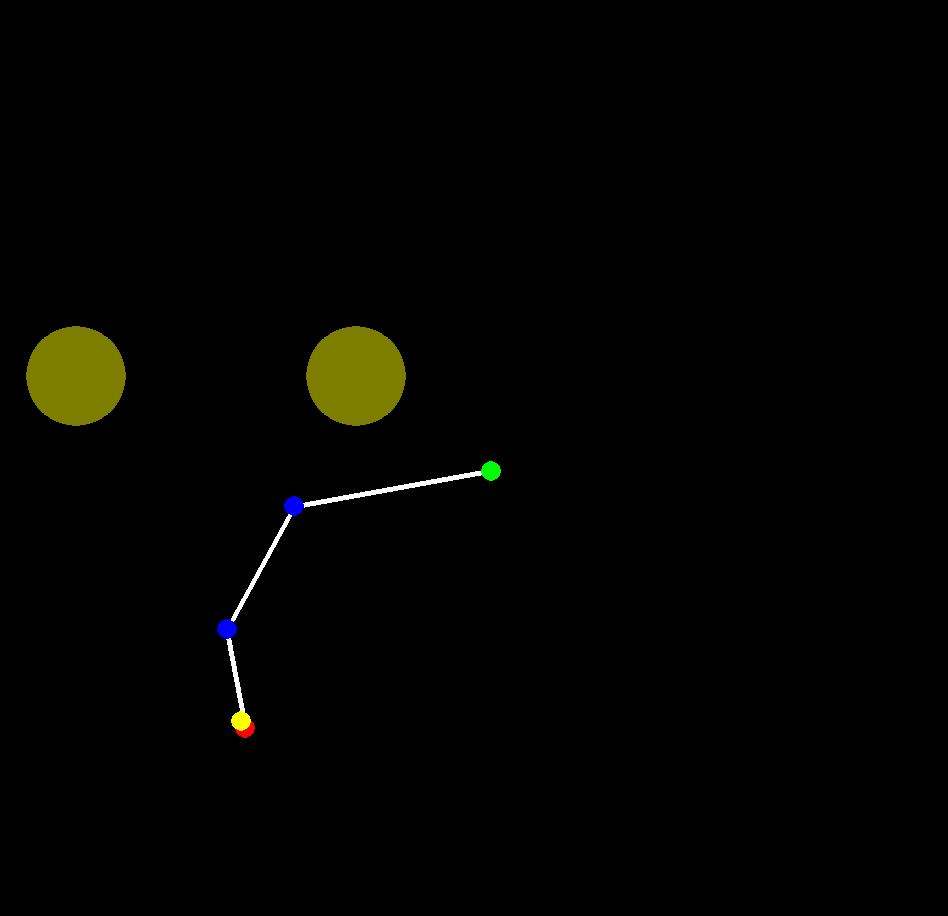
\includegraphics[scale=0.3]{img/ddpgfd_env.png}
	\caption{$\textit{Reacher}$ environment with two penalty areas.}
	\label{fig:ddpgfd0}
\end{figure}


% \begin{figure}[htbp]
% 	\centering
% 	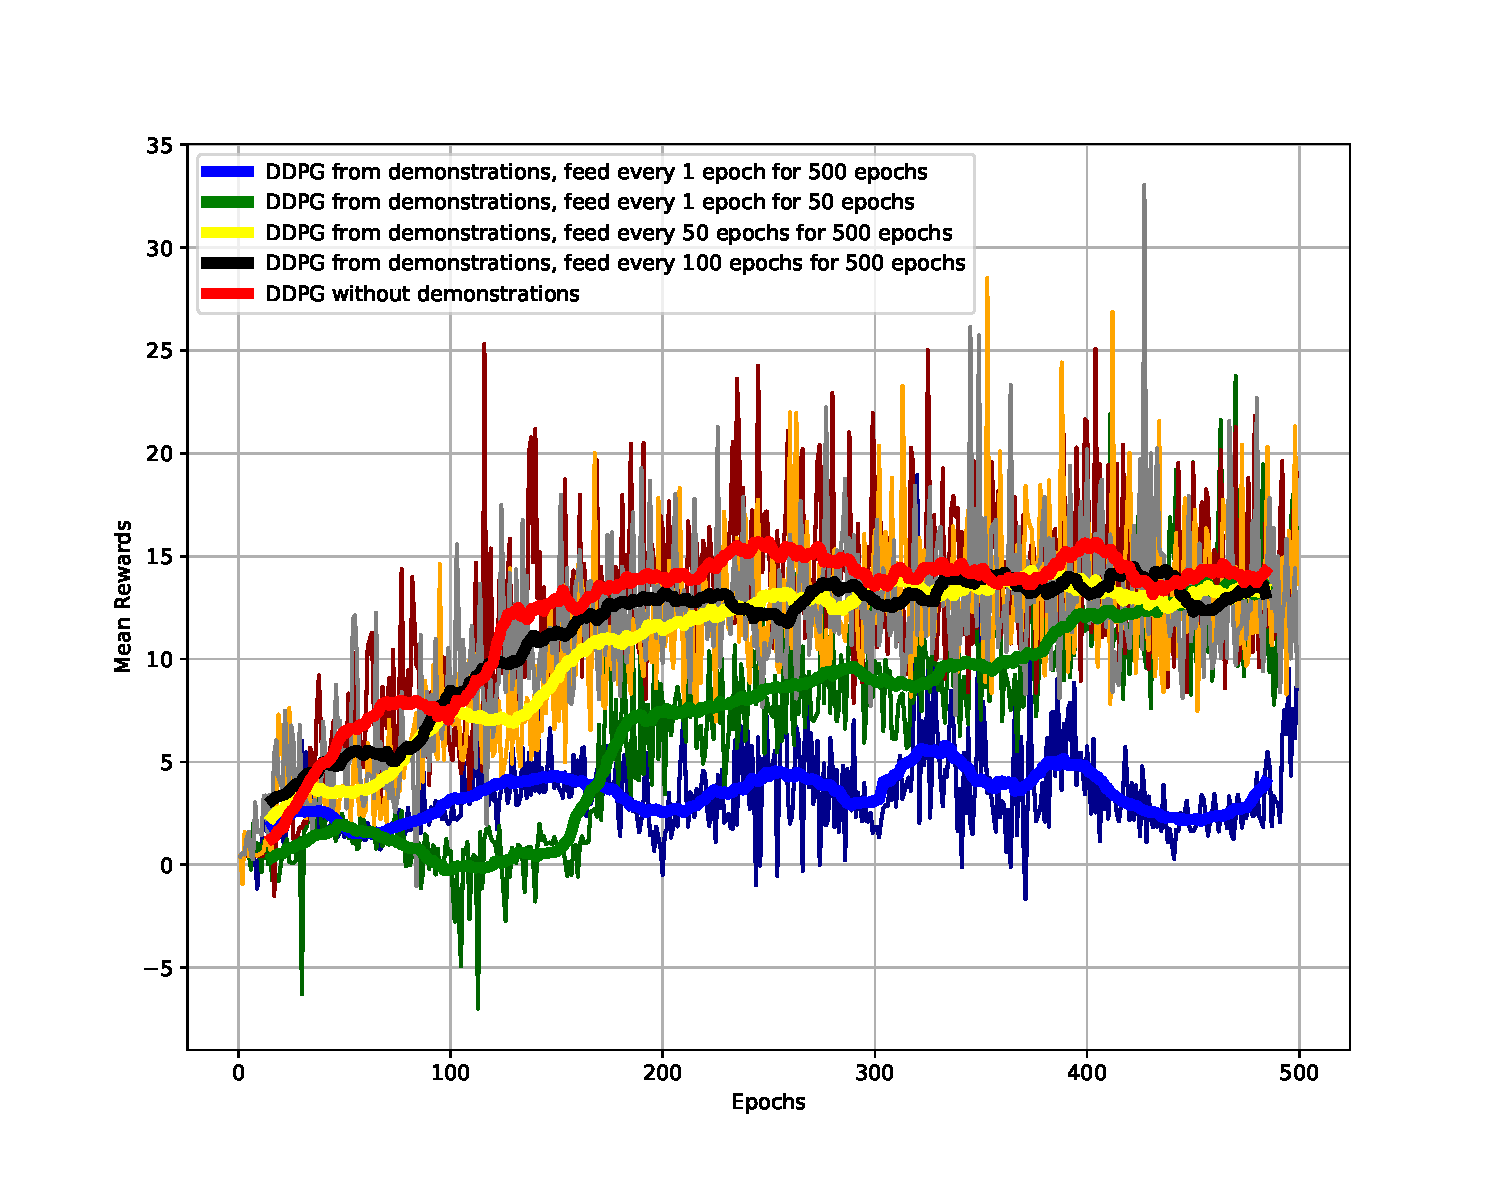
\includegraphics[scale=0.5]{img/ddpgfd1.pdf}
% 	\caption{Comparison of DDPG from demonstrations with different feeding approaches (without prioritized experience replay) and vanilla DDPG. The blue line is feeding demonstrations for every epoch for the whole training process (500 epochs); the green line is feeding demonstrations for every epoch for the first 50 epochs; the yellow line is feeding demonstrations for every 50 epochs for the whole training process; the black line is feeding demonstrations for every 100 epochs for the whole training process; the red line is vanilla DDPG without using demonstrations. }
% 	\label{fig:ddpgfd1}
% \end{figure}


\begin{figure}[htbp]
	\centering
	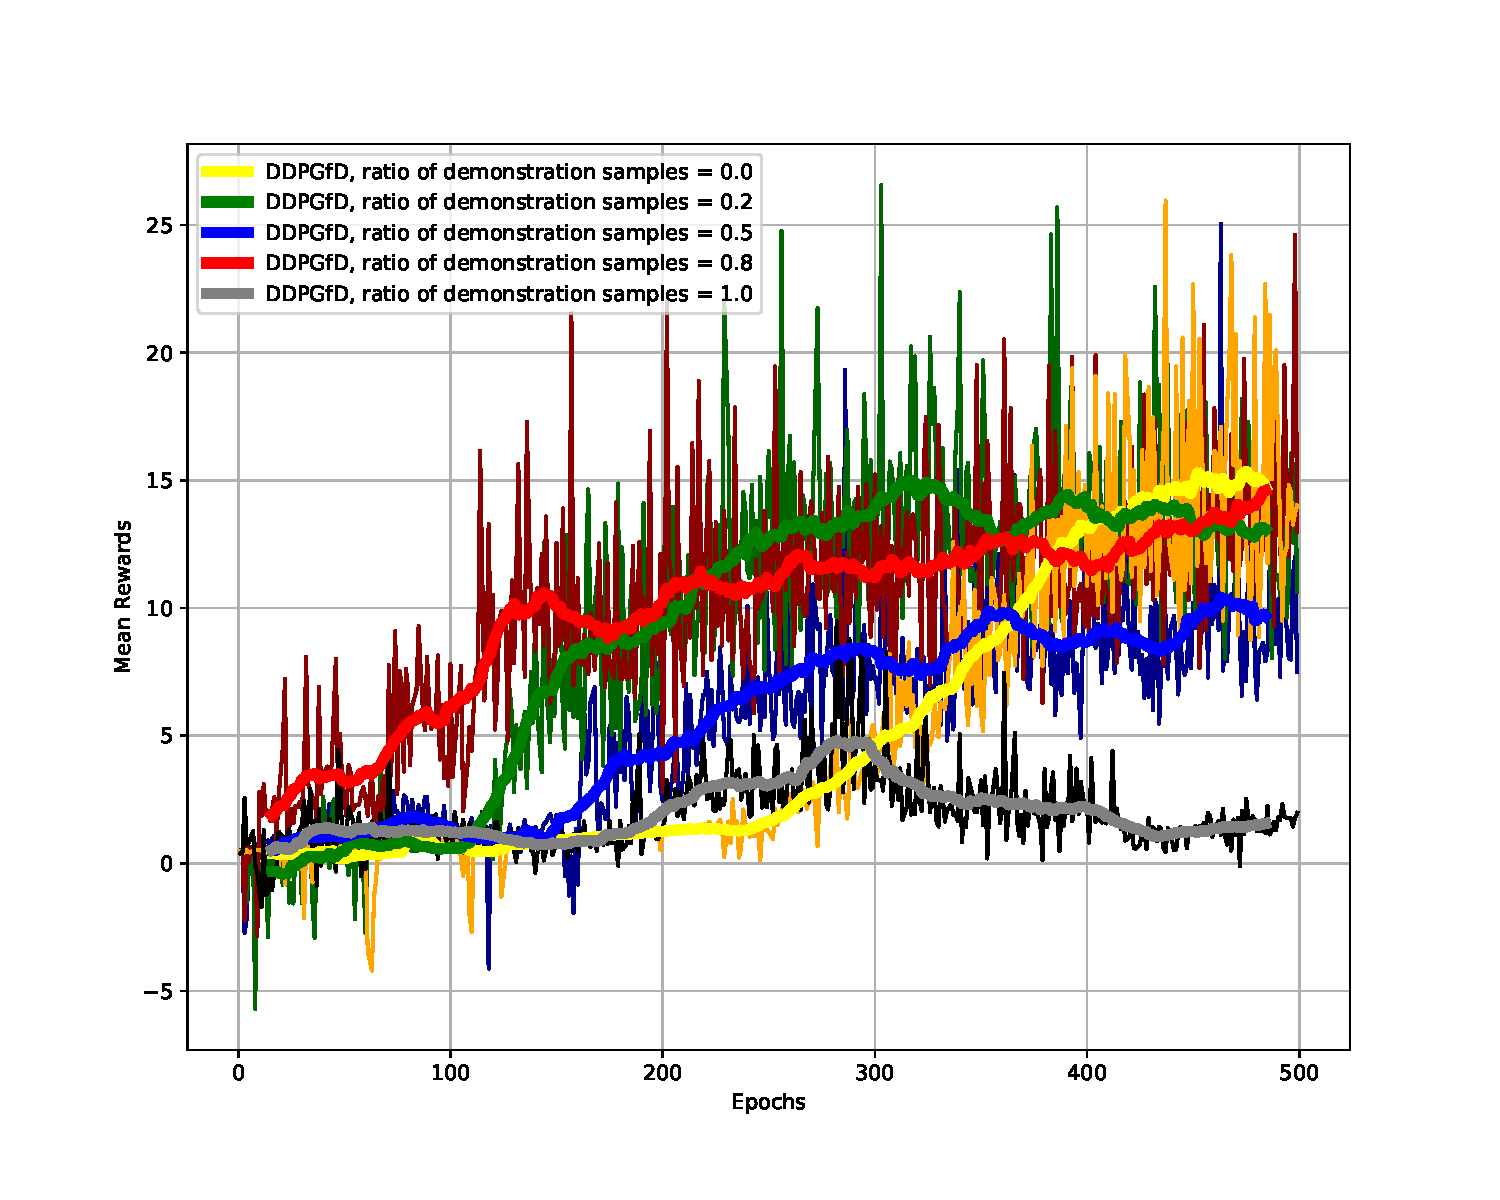
\includegraphics[height=250, width=400]{img/ddpgfd2.pdf}
	\caption{Results of DDPG from demonstrations with different ratios of demonstrations over all training samples. With demonstration sample ratio equivalent to 0.0, the DDPG policy actually learns from scratch without any demonstrations; and with the ratio equivalent to 1.0, it learns totally from the demonstrations without any samples from exploration. And in both of the above cases, the learning performance is as good as a proper ratio of demonstration between 0.0 and 1.0, e.g. 0.8.}
	\label{fig:ddpgfd2}
\end{figure}

\subsection{Benchmark Methods of Reinforcement Learning with Demonstrations}
\subsubsection{Variances in Experiments}
We first need to show the property of various and unstable performances in RL's training process, especially in algorithms like DDPG, etc. We take the residual policy learning with DDPG as example, displays the large variance in different trials of training. The unstable property of the learning process in RL contains several parts, including a non-converged optimal policy, large differences in performance of different trials, etc.

Experiments with three trials using residual policy learning for DDPG are shown in Fig. \ref{fig:variance}. We can see from the first two trials that some near optimal policies (as the black crosses in the figure) are learned at a relatively early learning stage with residual learning, but it does not converge to the policy and eventually learns a worse policy than that. And the third trial shows that the agent does not learn anything useful over the whole training epochs sometimes. Moreover, it shows that there is large performance variance in the learning process even with exactly the same methods and experimental settings, which is a typical property in experiments of RL. Therefore it will be common to see some large variances in experiment results shown in the following sections.

\begin{figure}[H]
	\centering
	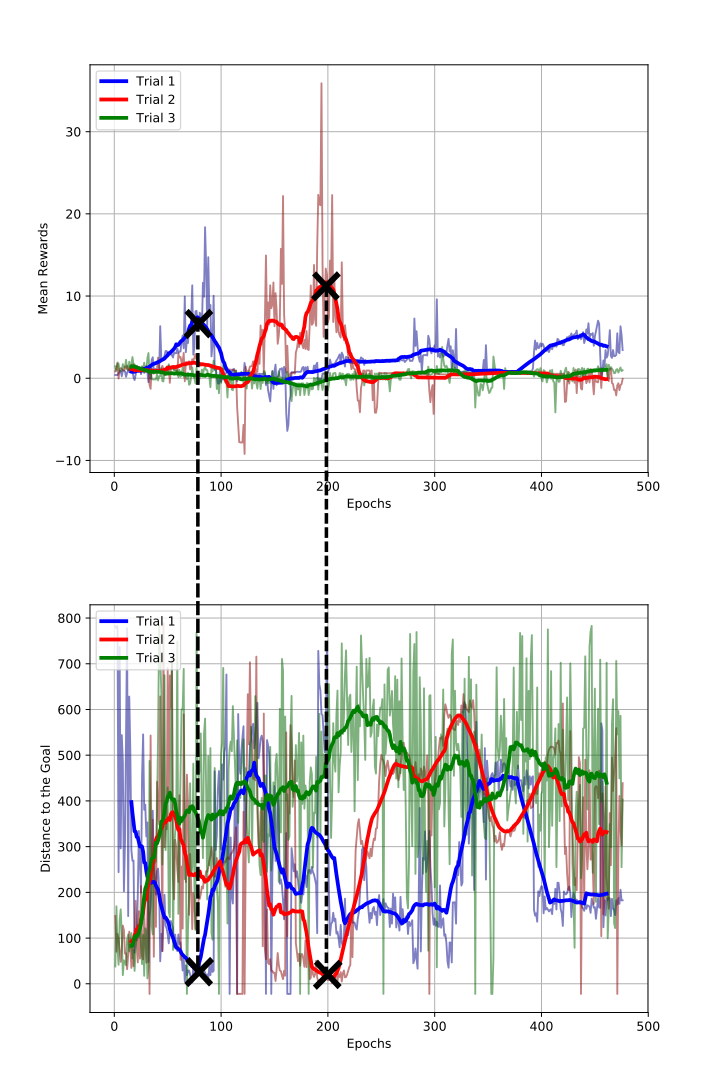
\includegraphics[scale=0.6]{img/variance.png}
	\caption{Variances of different trials in residual policy learning with DDPG in $\textit{Reacher}$ environment. There are three trials in above experiments. The figure on the top shows the mean reward over the training process; and the bottom one shows the distance of the end of reacher from the target goal during training epochs.}
	\label{fig:variance}
\end{figure}



\subsubsection{Comparisons of Methods for Reinforcement Learning with Demonstrations}
In this section, we display comparisons of experiment results with some of the above described efficient RL methods using demonstrations in the $\textit{Reacher}$ environment, including:

(1). policy replacement;

(2). residual policy learning;

(3). directly feeding demonstrations into the buffer. 

All methods are based on the same DDPG algorithm with same settings in hyper-parameters and neural network architectures, and they apply the same environment. We use general experiment settings which are used throughout this paper.

\textbf{General Experiment Settings}

* Environment: the leanring environment is a $\textit{Reacher}$ environment with 2 penalty areas of radius 50 as shown in Fig. \ref{fig:ddpgfd0} and joint length of $[200, 140, 100]$ with the screen size 1000, as described above.

* Neural networks: the actor network includes 5 fully connected layers with ReLu as hidden layer activation function and Tanh as output activation, and the size of each layer is 100 for the first 4 layer and 400 for the last layer. The critic network are almost the same just without activation for the last layer and so with Tanh for the last but one layers. The learning rate is $10^{-4}$ for the actor and $10^{-3}$ for the critic. Batchsize is 640, and exploration uses normal noise of scale 2.0 for experiments in Fig. \ref{fig:comparion3}.

* Dataset of demonstrations: we use two datasets of demonstrations, a small one and a large one. The small dataset contains 50 episodes of expert trajectories and the large one contains 1000 episodes, with 21 steps for each episodes. The demonstration trajectories are generated with a intermediate goal at between the two penalty areas via the inverse kinematics, and with injected normal noise. The demonstration data is used in several methods, including learning from demonstrations, pre-training the policy network as initialization and pre-training the policy network in residual learning.

* Training: both the initialization and residual learning methods are set to have a pre-heating process for training the critic, and the length of the pre-heating is 600 steps. The number of overall training steps is set to be $10^4$ for all methods.

\textbf{Experiments with Dense Rewards}

Comparison of different methods using demonstrations and dense reward function as in Eq.(\ref{equ:dense_reward}) with DDPG algorithm for $\textit{Reacher}$ environment are shown in Fig. \ref{fig:comparion3}, including policy replacement, residual policy learning and directly feeding demonstrations into the buffer (demonstration ratio: 0.5). We set the neural network architectures and other experiment parameters including the noise scale (=2.0) and activation function of output layer ($\alpha*$Tanh, $\alpha=30$) to be exactly the same for all the methods, including vanilla DDPG. For the method of residual policy learning, the residual policy network is set to be the same with actor policy networks in other methods. Experiments in Fig. \ref{fig:comparion3} shows that, directly feeding demonstrations into the memory buffer has more robust improvement in the learning process with general experiment settings, and the feeding ratio of demonstrations is 0.5 as default.
\begin{figure}[htbp]
	\centering
	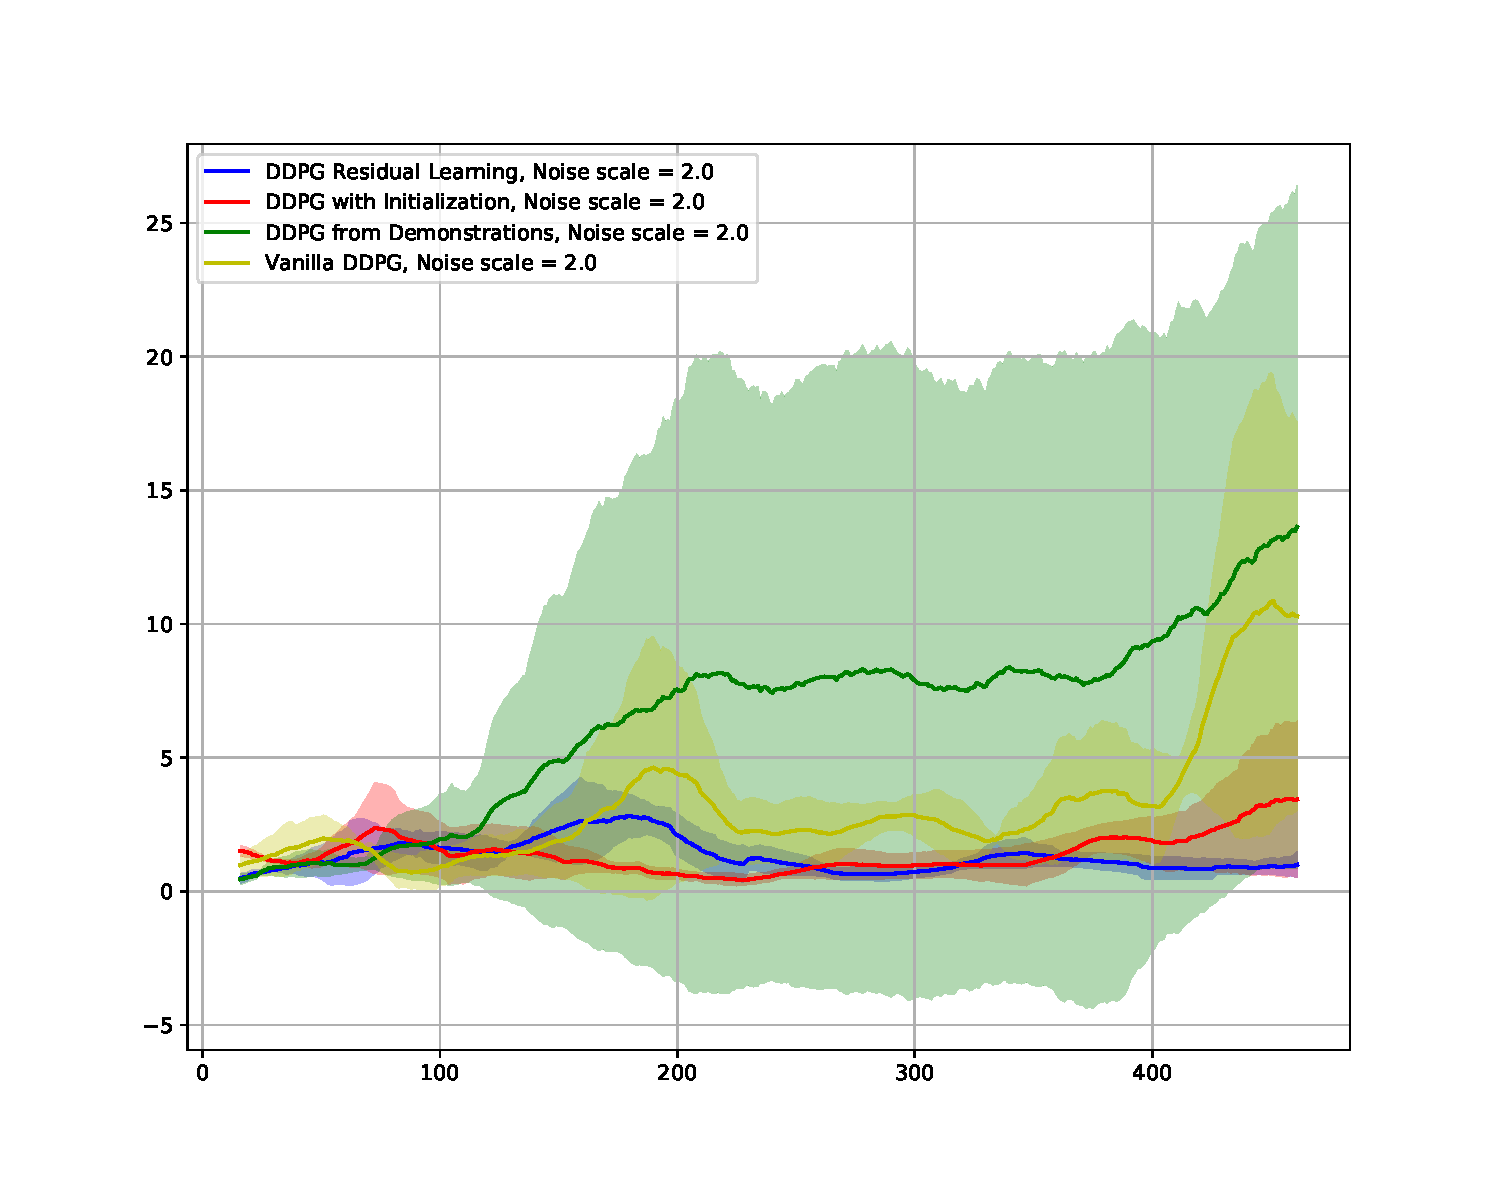
\includegraphics[height=250, width=400]{img/compare3.pdf}
	\caption{Comparison of different methods with demonstrations for efficient reinforcement learning (DDPG), including policy replacement, residual policy learning, directly feeding demonstrations (demonstration ratio: 0.5) into the buffer and vanilla DDPG. The overall length of training step is 10000, and there is a 600-step pre-heating process for policy replacement and residual policy learning.}
	\label{fig:comparion3}
\end{figure}

We also compare above methods with a same neural network architecture but different activation functions for the output layer and different hyperparameter settings, to fine-tune (showing the best performance) each method on the same $\textit{Reacher}$ task, as shown in Fig. \ref{fig:comparion4}. Different methods use different output activation functions, range of action values and noise scales, etc. The activation function of output layer of vanilla DDPG and policy replacement is the LeakyRelu function, while for the method of directly feeding demonstrations into memory buffer (DDPGfD) the function of $\alpha*$Tanh works more robustly and the $\alpha$ (=30) is a factor of value range. And for the residual learning, Tanh activation function in the output layer is used for the initialized policy but is easily saturated for the resisual polciy in experiments, therefore we apply an activation function of LeakyRelu6 (LeakyRelu with a clip on positive axis of range [0,6]) with a scaling parameter $\alpha(=0.2)$ for the residual policy. Therefore the action value range of the residual policy is much smaller than a general action policy, which indicates a delicate learning upon a good initialization policy. Actually, the better the initialization policy, the smaller the range of both action value and noise scale is needed for residual learning, which is explained in the section of residual policy learning. Moreover, different methods use different noise scale for their own benefits as shown in the figures. Then uninitialized policy tends to use a larger noise scale for better exploration, while the initialized policy like the residual learning uses a smaller noise scale as it only learns a residual upon a pre-trained policy.

Two figures are shown in Fig. \ref{fig:comparion4}, the mean episode reward versus training epochs and the final distance of the end of reacher to the goal position versus training epochs. As different methods requires different experiment settings including the outputs of the learned policy (e.g. the action values in the residual learning are affected by two policies, and they may have different ranges of action value compared with other methods, which will cause the pace of the reacher's motion and average episode rewards to be different), it is not a fair comparison with only the figure of mean episode reward. Therefore we show an additional figure of final distance to the goal position. And there are some other cases may cause the discrepancies in the two figures in Fig. \ref{fig:comparion4}: sometimes the reacher may go through the goal position but not stay at it until the end of an episode and still get a relatively large reward; and sometimes the reacher reaches the final goal position but through the penalty areas with a relatively small episode reward.


\begin{figure}[H]
	\centering
	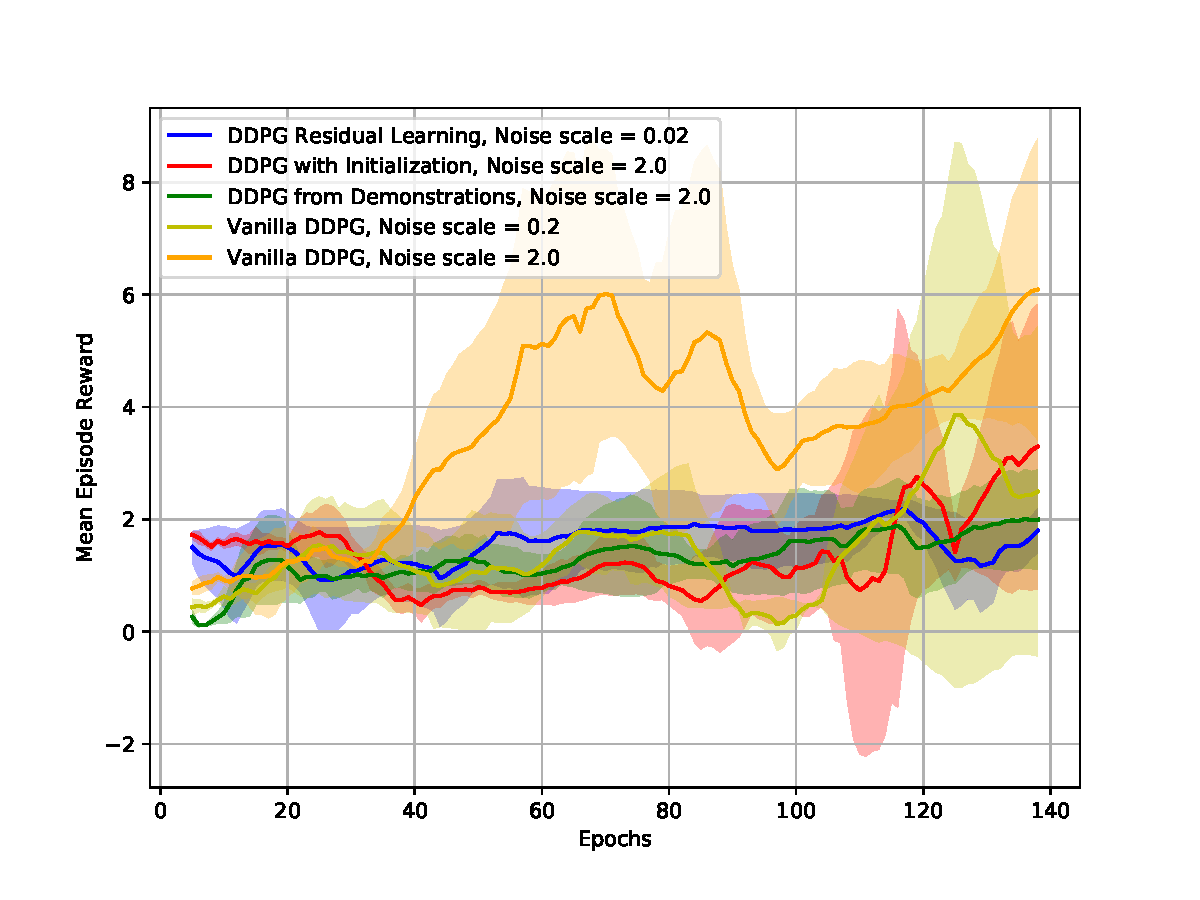
\includegraphics[scale=0.5]{img/3000step31.pdf}
	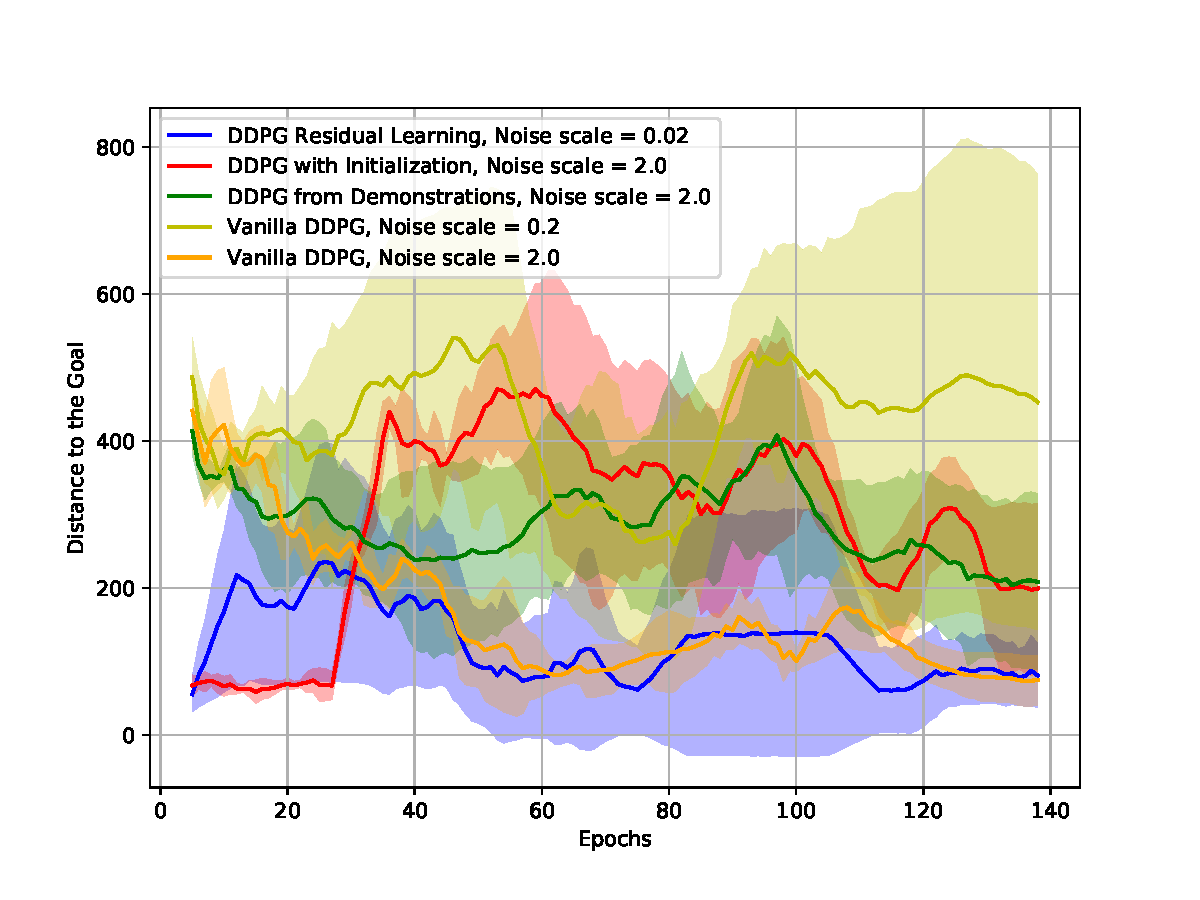
\includegraphics[scale=0.5]{img/3000step41.pdf}
	\caption{Early stage of training performances of different methods for efficient reinforcement learning (DDPG) with \textbf{dense reward} function, using different parameter settings (e.g. output layers of neural networks, noise scales, etc), including policy replacement, residual policy learning, directly feeding demonstrations into the buffer ((demonstration ratio: 0.5)) and vanilla DDPG. Each method is tested with three trials on the same environment. The overall length of training step is 3000, and there is a 600-step (28 epochs) pre-heating process for policy replacement and residual policy learning. The above figure is the mean episode reward versus the training epoch, and the one below is the final distance to goal position for each episode versus the training epoch. We can see from the second figure that the residual policy learning actually performs well with fine-tuning, as it learns upon a good initialization policy.}
	\label{fig:comparion4}
\end{figure}

\textbf{Experiment with Sparse Reward}

Experiments above uses dense reward function as in Eq.(\ref{equ:dense_reward}). In this section, we show comparisons of different methods with the sparse reward function defined as follows (mentioned in former sections):
\begin{equation}
    R =
\begin{cases}
R_T& \sqrt{(x_3-x_T)^2+(y_3-y_T)^2}<r_T\\
R_P& \sqrt{(x_3-x_P)^2+(y_3-y_P)^2}<r_P\\
-1& \text{Otherwise}
\end{cases}
\end{equation}
where $R_T=20, R_P=-5, r_T=30$ in experiments, and $r_P$ is the radius of penalty areas equivalent to 50.
Experiment results are shown in Fig. \ref{fig:comparion5} with fine-tuning for each methods, including policy replacement, residual policy learning, directly feeding demonstrations into the buffer ((demonstration ratio: 0.5)) and vanilla DDPG. Basic settings of it is the same as the experiments shown in Fig. \ref{fig:comparion4} in the above section with dense reward function. The residual policy learning with fine-tuning still performs the best as shown in the distance figure. And both methods of directly feeding demonstrations into memory and policy replacement show improvement in learning performance, the former one is better in learning effective trajectories. 

Note that there are two unusual points in the Fig. \ref{fig:comparion5}: (1). the large reward with the approach of feeding demonstrations in the above figure is because of its $30*$ Tanh (a relatively large action value makes the agent reach the goal faster) activation function for output layer. (2). as the noise scale is different in different methods, the final distance to the goal position is supposed to be larger on average in training with methods using relatively large noise scale like policy replacement and demonstrations feeding approaches, compared with residual policy learning, even their policy performances may be similar in test without noise (e.g. they can all reach the goal quickly). 

As for vanilla DDPG, it generally cannot learn anything useful in a training scope of 3000 steps. Therefore, above three methods for leveraging demonstrations actually have more significant improvement in learning performance with sparse reward than with dense reward.

\begin{figure}[H]
	\centering
	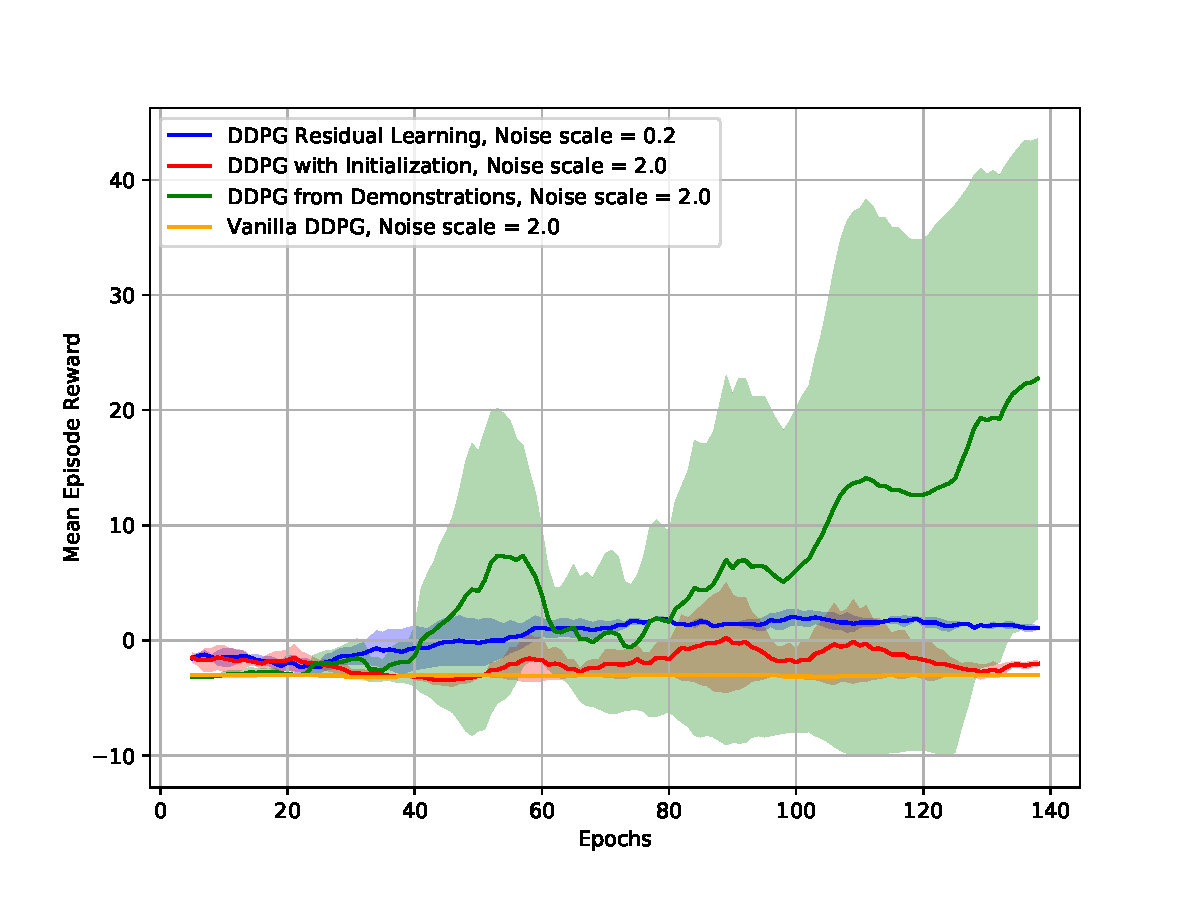
\includegraphics[scale=0.5]{img/3000step_sparse1.pdf}
	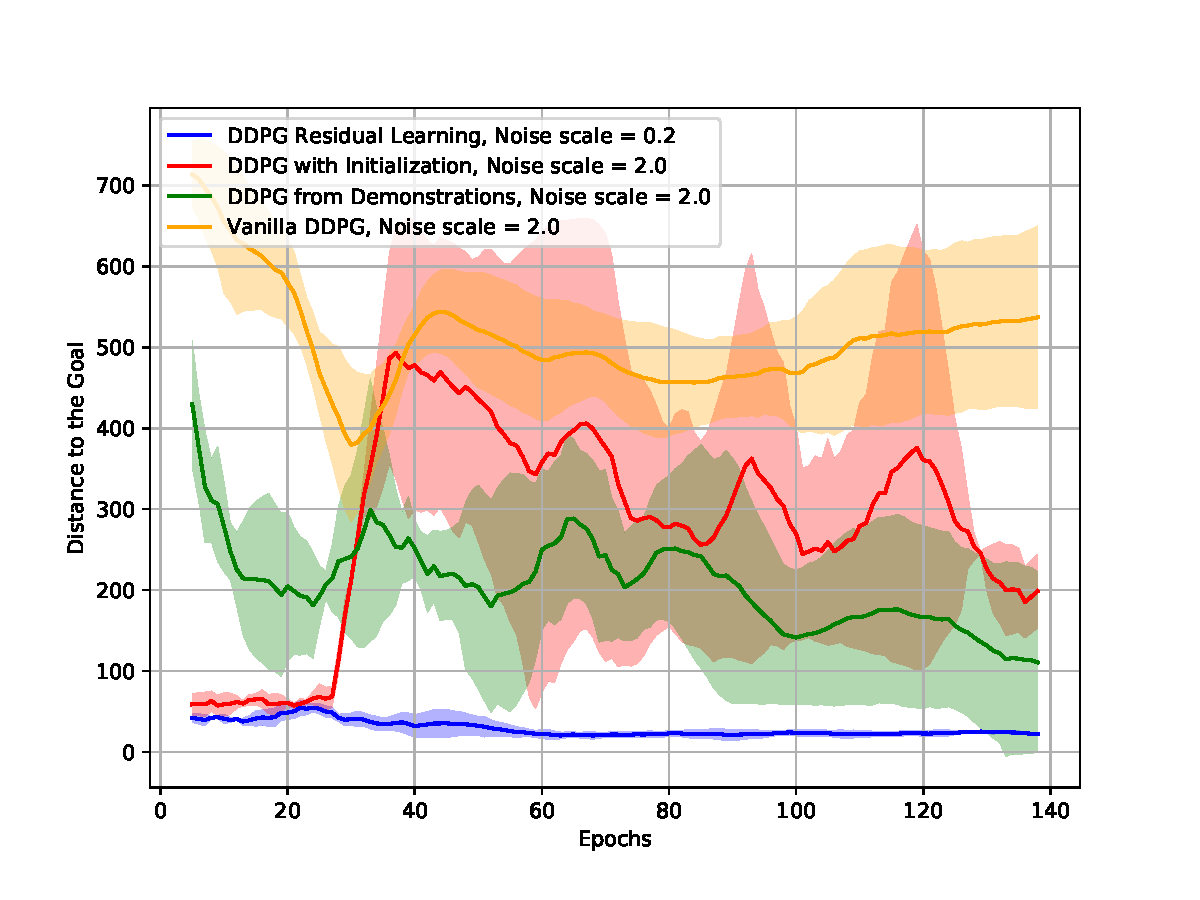
\includegraphics[scale=0.5]{img/3000step_sparse2.pdf}
	\caption{Early stage of training performances of different methods for efficient reinforcement learning (DDPG) with \textbf{sparse reward} function, using different parameter settings (e.g. output layers of neural networks, noise scales, etc), including policy replacement, residual policy learning, directly feeding demonstrations into the buffer ((demonstration ratio: 0.5)) and vanilla DDPG. Each method is tested with three trials on the same environment. The overall length of training step is 3000, and there is a 600-step (28 epochs) pre-heating process for policy replacement and residual policy learning. The above figure is the mean episode reward versus the training epoch, and the one below is the final distance to goal position for each episode versus the training epoch. }
	\label{fig:comparion5}
\end{figure}

\textbf{Experiment with Small Set of Demonstrations}

We use the large dataset with 1000 demonstrations in above experiments. And in this section we wonder if there is any bad effects if we use a smaller dataset, containing only 50 demonstrations, which can be derived easily even in real world scenario with human experts. All experiment settings are remained the same as above sections. And the reduction in demonstration dataset actually only affects the method with policy replacement as initialization and the residual policy learning, because the initialization policy will be different for these two approaches. As for the approach of feeding demonstrations into memory, it should not be affected as long as the number of demonstrations fed into the memory is sufficient for the sampling process of training, because those demonstrations are all generated by expert policy with random noise and the number of it does not matter. We also use sparse reward function in this experiment.

Experiment results are shown in Fig. \ref{fig:comparion6}. Compared with applying a large demonstration dataset in Fig. \ref{fig:comparion5}, no prominent bad effects are displayed through the experiments for those initialized policy methods.

\begin{figure}[htbp]
	\centering
	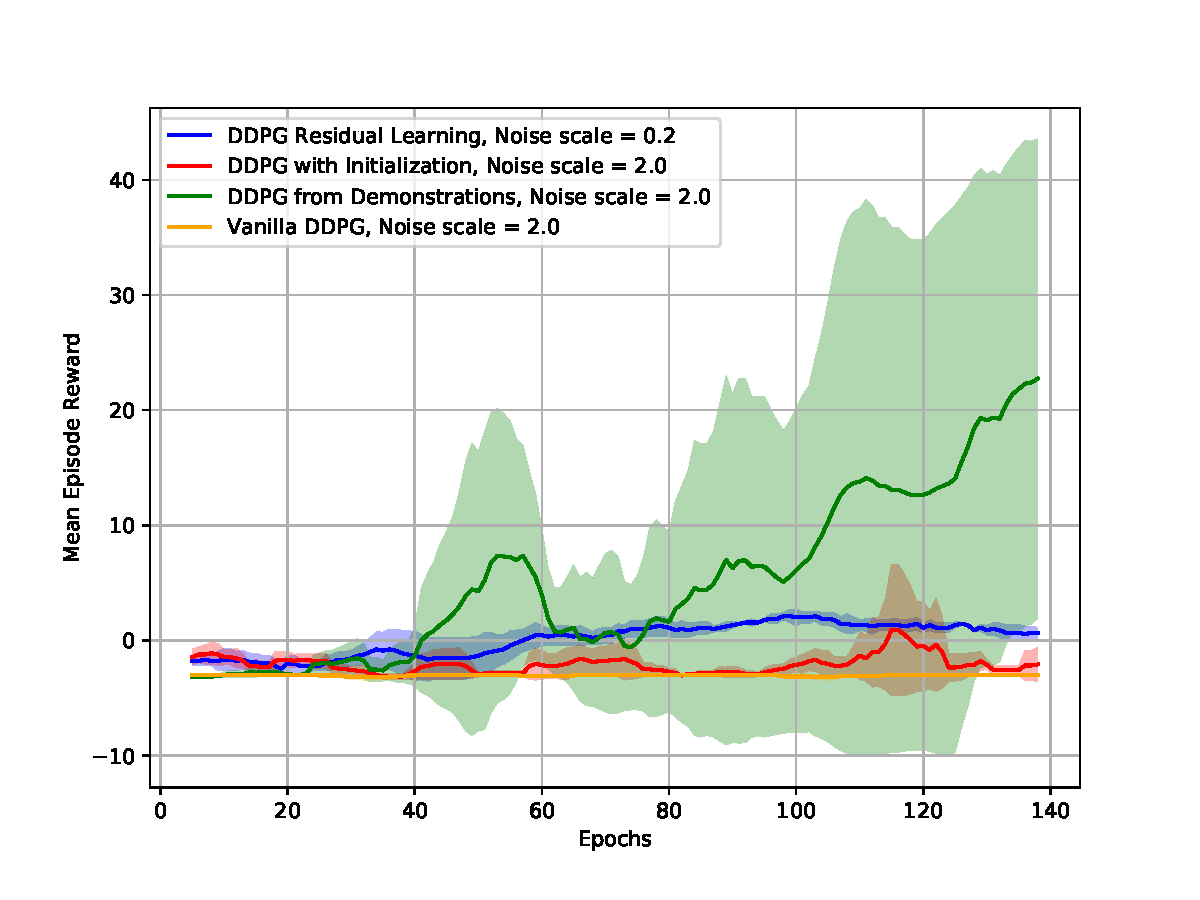
\includegraphics[scale=0.5]{img/3000step_smalldemon1.pdf}
	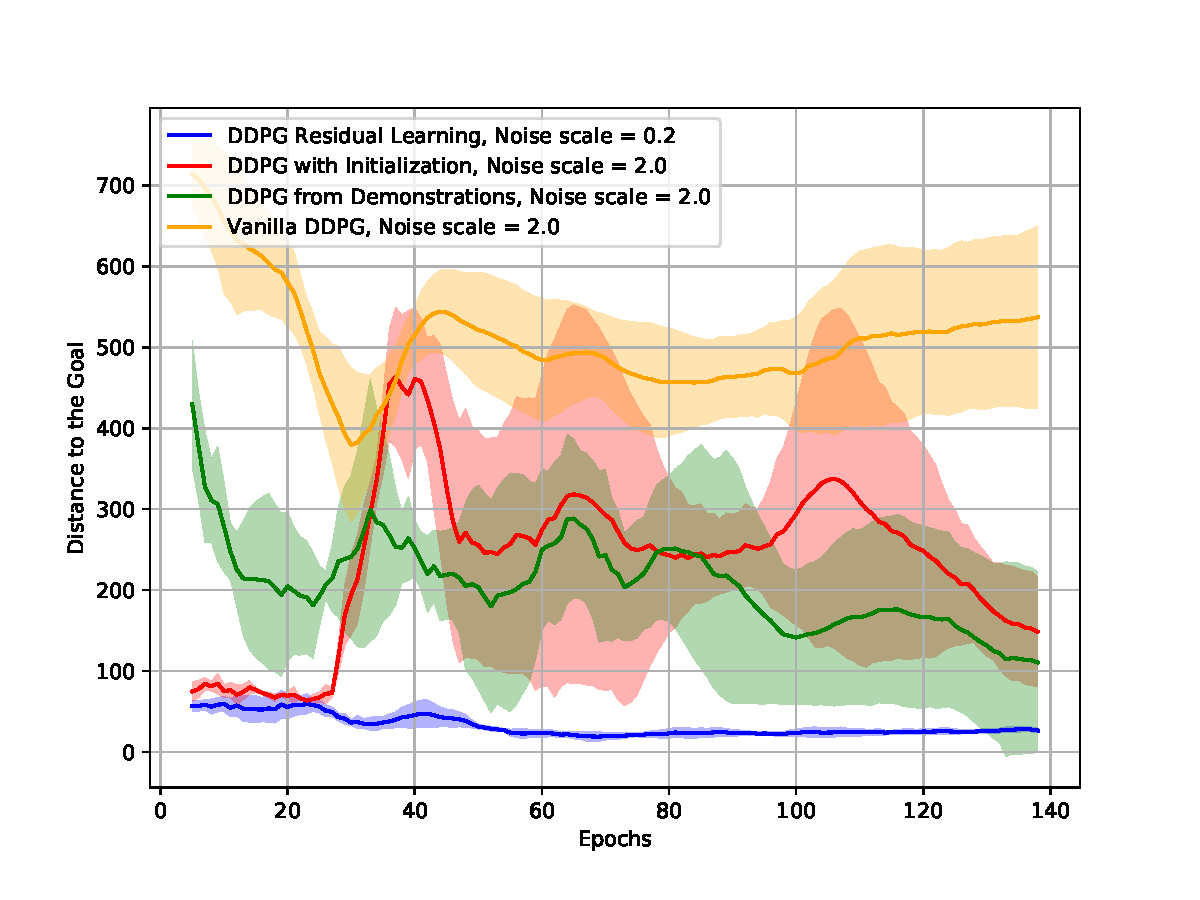
\includegraphics[scale=0.5]{img/3000step_smalldemon2.pdf}
	\caption{Early stage of training performances of different methods for efficient reinforcement learning (DDPG) with sparse reward function and \textbf{small dataset of demonstrations (50)}, using different parameter settings (e.g. output layers of neural networks, noise scales, etc), including policy replacement, residual policy learning, directly feeding demonstrations into the buffer (demonstration ratio: 0.5) and vanilla DDPG. Each method is tested with three trials on the same environment. The overall length of training step is 3000, and there is a 600-step (28 epochs) pre-heating process for policy replacement and residual policy learning. The above figure is the mean episode reward versus the training epoch, and the one below is the final distance to goal position for each episode versus the training epoch. We can see from the second figure that the residual policy learning actually performs well with fine-tuning, as it learns upon a good initialization policy.}
	\label{fig:comparion6}
\end{figure}



\subsubsection{Conclusions from Experiments}

Some conclusions can be derived from above experiments using described three approaches for leveraging demonstrations in RL process, as listed in the following:

1. The approach of learning with demonstrations fed directly into the memory buffer shows robust improvement in performance with general experiment settings;

2. The approach of residual policy learning works the best with fine-tuning and good initialization policy, benefiting from the restricted exploration range (sometimes manually set according to the performance of initialization policy) of the residual policy;

3. Vanilla DDPG could work well with dense reward function, but much worse with sparse reward function, even learn nothing useful in the early training stage;

4. The effect of improvement in learning performance using above methods for leveraging demonstrations, including policy replacement, residual policy learning and directly feeding demonstrations into memory, is more prominent with sparse reward function than with dense reward.

5. There is no prominent bad effects when the demonstration dataset for training the initialization policy using supervised imitation learning is small, for the case of sparse reward function. And the case of dense reward function is supposed to be similar. But of course, if the demonstration dataset is too large (if covering most cases of the action space, it could be directly used as the policy without RL) or too small (e.g. 1 or 2 demonstrations), it could make some differences.

\subsection{Other Methods for Efficient Reinforcement Learning with Demonstrations}

\subsubsection{Deep Q-Learning from Demonstrations}
Deep Q-Learning from Demonstrations (DQfD) \cite{hester2018deep} is a method similar with the DDPGfD method as described in the above sections, but applies DQN for only discrete action space applications. DQfD also applies the prioritized experience replay to leverage a small set of demonstrations, and DQfD trains the policy using a combination of a supervised hinge loss for imitating the demonstrations and a general TD loss.

\subsubsection{Normalized Actor-Critic}
Normalized Actor-Critic (NAC) \cite{gao2018reinforcement} is another method for efficient RL with demonstrations, and it pre-train a policy as initialization for a refinement RL process. The key difference of NAC from other methods is that it uses exactly the same objective for the processes of pre-training an initialization policy with demonstrations and the refinement RL learning process (not like a combination of supervised loss and RL loss in DQfD, or two separate training processes with different loss in policy replacement and behavioral cloning methods), which makes NAC robust to suboptimal demonstrations data.

NAC method is similar to methods of DDPGfD or DQfD, but trains the policy sequentially from demonstrations and samples from interactions instead of using samples from both sources at the same time.

\subsubsection{Reward Shaping with Demonstrations}
Reward shaping with demonstrations \cite{brys2015reinforcement} is a method focusing on the initialization of value-evaluation function instead of the action policy for RL. It provides the agent an intermediate reward for enriching the sparse reward signals:
\begin{equation}
    R_F(s,a,s')=R(s,a,s')+F^D(s,a,s')
\end{equation}
where the shaping reward $F^D$ from demonstrations $D$ is defined with potential function $\phi$ in the following form to guarantee the convergence:
\begin{equation}
    F^D(s,a,s',a')=\gamma \phi^D(s',a')-\phi^D(s,a)
\end{equation}
and $\phi^D$ is defined as:
\begin{equation}
    \phi^D(s,a)=\max_{(s^d, a)}e^{-\frac{1}{2}(s-s^d)^T\Sigma^{-1}(s-s^d)}
\end{equation}
which is to maximize the value of the potential for the state $s$ that is most similar as the demonstration state $s^d$. And the optimized potential function is used to initialize the action-value function $Q$ in RL:
\begin{equation}
 Q_0(s,a)=\phi^D(s,a)   
\end{equation}
The intuition of reward shaping method is to bias the exploration in favour of those state-action pairs in demonstrations or close to those in demonstrations for accelerating the training process of RL. Reward shaping provides a good approach of initialization for the value-evaluation function in RL process. 

Other methods like unsupervised perceptual rewards \cite{sermanet2016unsupervised} also learns a dense and smooth reward functions with the demonstrations, using features in a pre-trained deep models.

\subsubsection{Optimistic Initialization}
Optimistic initialization is usually used in RL for boosting explorations \cite{sutton2018reinforcement}, which helps trade off between exploration and exploitation in the training stage of RL. Domain-independent optimistic initialization \cite{machado2015domain} shifts the reward function $r_t$ with the first reward $r_{1st}$ in an episode as $r_t/|r_{1st}|$ and downward it by $\gamma-1$, where $\gamma$ is the factor for reward discounting. Therefore $\Tilde{r_t}=\frac{r_t}{r_{1st}}+(\gamma-1)$, and the corresponding value function is:
\begin{equation}
\begin{aligned}
    \Tilde{Q}_\pi(s_t,a_t)&=\mathbb{E}_\pi[\sum_{k=0}^\infty\gamma^k\Tilde{r}_{t+k+1}]\\
    &=\mathbb{E}_\pi[\sum_{k=0}^\infty\gamma^k\frac{r_{t+k+1}}{|r_{1st}}+\sum_{k=0}^\infty\gamma^k(\gamma-1)]
\end{aligned}
\end{equation}
Above domain-independent optimistic initialization provides an approach to normalize the reward function without domain knowledge. However, we can also apply demonstrations data for optimistic initialization for better learning performance in a specific task domain. 


\section{Efficient Reinforcement Learning without Demonstrations}
\subsection{Meta-learning as Initialization for Reinforcement Learning}
Meta-learning is also called learning to learn, lifelong learning, transfer learning, multi-task learning, etc. The goal of meta-learning is to learn transferable knowledge which can be generalized in multi-tasks, so as to accelerate the learning process in some computationally expensive tasks especially like reinforcement learning. Present meta-learning algorithms in reinforcement learning domain include model-agnostic meta-learning (MAML) \cite{finn2017model}, Reptile \cite{nichol2018first}, E-MAML \cite{stadie2018some} and E-RL$^2$ \cite{stadie2018some}, probabilistic MAML \cite{finn2018probabilistic}, Multi-Modal Model-Agnostic Meta-Learner (MuMoMAML) \cite{vuorio2018toward}, Meta-Imitation Learning with MAML \cite{finn2017one}\cite{yu2018one}, and LSTM based methods \cite{ravi2016optimization} like RL$^2$ \cite{duan2016rl}, Learn to RL \cite{wang2016learning}, Learning to Learn by Gradient Descent by Gradient Descent \cite{andrychowicz2016learning}, and meta-leaner with attention strategy like Simple Neural Attentive Learner (SNAIL) \cite{mishra2017simple}, etc. Some works point out potential problems of MAML like negative adaptation problem \cite{deleu2018effects} and unstable training problems of MAML \cite{antoniou2018train}. Modifications of MAML like MAML++ \cite{antoniou2018train} for better performance and more stable training process are on the way.

Meta-learning can not only be applied on supervised learning problems, but also on RL problems, which is meta-RL. And meta-RL can be used in tasks like robotic control for improving the learning efficiency.

Task settings: as meta-learning is to learn across tasks, it is usually computationally expensive, especially for reinforcement learning tasks. In order to simplify the tasks, we reduce the number of joints in $\textit{Reacher}$ from 3 to 2 in experiments. And the difference of tasks in a specific task domain is set to be the different positions of the target point. 
\subsubsection{First and Second Order Modal-Agnostic Meta-Learning Algorithms}
\textbf{MAML}

MAML \cite{finn2017model} is meta-learning method to unroll the computation graph with second derivatives for updating the meta policy across tasks. And it has an approximate version called first-order MAML (FOMAML) by just ignoring the second-order term. The updated policies of MAML contains an inner policy, which is a task-specific policy, and an outer policy, which is the meta policy. The goal of MAML is to learn a better meta policy for accelerating the learning process of every task-specific policies. 

MAML can be regarded as updating the meta-policy according to the test error with updated parameters (according to the training error on old samples) on new samples. The update rule of the inner policy is a general one (w.r.t. the training error), for task $\mathcal{T}_i$ sampled from the task domain:
\begin{equation}
    \theta_i' = \theta - \alpha \nabla_{\theta}L_{\mathcal{T}_i}(f_{\theta})
\end{equation}
and for the outer policy update (w.r.t. the test error on the new samples with updated parameters in inner update):
\begin{equation}
\label{equ:maml_update}
    \theta \leftarrow \theta - \beta\nabla_{\theta}\sum_{\mathcal{T}_i\sim p(\mathcal{T})}L_{\mathcal{T}_i}(f_\theta_i')
\end{equation}
where the $\alpha, \beta$ are stepsize variables, the $\theta, \theta_i$ are parameters of the parameterization function $f$ for the meta policy and policy of task $\mathcal{T}_i$ respectively (e.g. $f_\theta$ is policy $\pi_\theta$ parameterized by $\theta$). 
The loss function $L$ for task $\mathcal{T}_i$ with parameterized policy $f_\theta$ is generally:
\begin{equation}
    L_{\mathcal{T}_i}(f_\theta) =\int R_{\mathcal{T}_i}(t) f_\theta(t) dt
\end{equation}
and in RL algorithms like PPO:
\begin{equation}
\label{equ:1}
     L_{\mathcal{T}_i}(\pi_\theta) = \mathbb{E}[\log \pi_\theta(a|s)\cdot A_{\mathcal{T}_i}(s)]
\end{equation}
where $A(s)$ is advantage function of state $s$.

\textbf{FOMAML}

FOMAML is a simplified version of MAML with only the first order derivatives of MAML. Therefore it is computationally more efficient than MAML. The update rules for FOMAML are:
\begin{equation}
    \theta_i' = \theta - \alpha \nabla_{\theta}L_{\mathcal{T}_i}(f_{\theta})
\end{equation}
\begin{equation}
    \theta \leftarrow \theta - \beta\sum_{\mathcal{T}_i\sim p(\mathcal{T})} \nabla_{\theta_i'}L_{\mathcal{T}_i}(f_\theta_i')
\end{equation}
for inner policy and outer policy update respectively.

\textbf{Reptile}

Reptile \cite{nichol2018first} is another meta-learning algorithm with only first-order derivatives similar to FOMAML for meta-learning with only first-order gradients. The update rule for Reptile is as follows:

For task $\mathcal{T}_i$, 
\begin{equation}
        \theta_i' = \theta - \alpha \nabla_{\theta}L_{\mathcal{T}_i}(f_{\theta})
\end{equation}
\begin{equation}
   \theta \leftarrow \theta + \epsilon ( \theta_i'-\theta)
\end{equation}
Note that the first step of above update in Reptile is usually a k-step update and here just show a one-step update. 

\textbf{MuMoMAML}

MuMoMAML \cite{vuorio2018toward} applies an extra model-based meta-learner on top of the gradient-based meta-learner in general MAML algorithms, which consists of an additional update of the modulation parameters $\omega$ in the outer policy update step :
\begin{equation}
    \omega \leftarrow \omega - \beta\nabla_{\omega}\sum_{\mathcal{T}_i\sim p(\mathcal{T})}L_{\mathcal{T}_i}(f_\theta_i', \tau)
\end{equation}
where $\tau = g(\{x,y\}; \omega)$ and it is used for modulating the prior parameters of the gradient-based meta-learner with respect to the task specification data $\{x,y\}$, using the following equations:
\begin{equation}
    \phi_i = \theta_i \bigdot \tau_i 
\end{equation}
and in MuMoMAML the gradient-based meta-learner uses the
modulated prior parameters $\phi_i$ instead of the original parameters $\theta_i$. The intuition of the MuMoMAML is to let the gradient-based meta-learner in MAML be aware of the task specification with the help of the model-based meta-learner. 

\textbf{E-MAML}

The E-MAML \cite{stadie2018some} algorithm changes the meta-policy loss function of MAML to be:
\begin{equation}
     L_{\mathcal{T}_i}(\pi_{\theta '}) = \mathbb{E}[\log \pi_{\theta '}(a|s)\cdot A_{\mathcal{T}_i}(s)
     + \lambda\cdot A_{\mathcal{T}_i}(s) \cdot \sum_{s\sim \pi_\theta}\log \pi_\theta (a|s)]
\end{equation}
in which it applies an interpretation of a stochastic gradient update of inner policy instead of the deterministic one in conventional MAML. And the $\lambda$ is a trade-off parameter for smoothly tuning between the stochastic treatment and non-stochastic treatment of the inner loop policy update.

Directly optimizing original MAML loss function like Eq.(\ref{equ:1}) will not account for the impact of the original sampling distributions $\pi_\theta$ on the future rewards $R(t)$ on trajectories with updated (in inner loop) policy $\pi_{\theta '}$. The effect of the additional second term in E-MAML is to make the policy more exploratory.

\textbf{Meta-Imitation Learning with MAML}

Meta-Imitation Learning with MAML \cite{finn2017one} is a another version of MAML algorithm for imitation learning with expert demonstrations. The difference of Meta-Imitation Learning with MAML from MAML is just the learning samples are from expert demonstrations instead of samples with current policy. The test error (outer policy) on expert demonstrations is the training error of the meta-learning.

\textbf{Negative Adaptation in MAML}

Tristan et al. \cite{deleu2018effects} points out the adaptation phase (the inner policy update) in MAML update as in Eq.(\ref{equ:maml_update})has no guarantee to show improvement on an individual task,  which could significantly decrease the performance on continuous control problems. The reason of it is that the meta-update in MAML encourages the adapted policy $\pi_{\theta'_\mathcal{T}}$ to have larger expected return while not considering the initial policy $\pi_{\theta_\mathcal{T}}$ before the adaptation phase. Therefore \textbf{the adapted policy $\pi_{\theta'_\mathcal{T}}$ may perform worse than the initial policy $\pi_{\theta_\mathcal{T}}$, which is called the negative adaptation}. And the authors propose a constraint on the meta-policy update:
\begin{equation}
    \min_\theta\mathbb{E}_{\mathcal{T}\sim P(\mathcal{T})}[L(g(\mathcal{D_{\mathcal{T}};\theta});\mathcal{D}'_{\mathcal{T}})] \quad \text{s.t.} P(P(\Gamma_\mathcal{T}(\theta)\leq 0)\leq 1-\beta)\leq 1-\delta
\end{equation}
where $\mathcal{D_{\mathcal{T}}}, \mathcal{D‘_{\mathcal{T}}}$ are data trajectories sampled from before and after the adaptation phase for task $\mathcal{T}$, $g$ is the gradient function, and $\beta, \delta$ are improvement factors for the level of a specific task and for overall tasks respectively. $\Gamma_{\mathcal{T}}(\theta)$ is a function measuring the update of policy:
\begin{equation}
    \Gamma_{\mathcal{T}}(\theta)=G_0(\pi_{\theta_\mathcal{T}})-G_0(\pi_{\theta'_\mathcal{T}})
\end{equation}
and $G_0$ is a value function for measuring the expected return.

\subsubsection{Understandings about Meta-Learning}
We first need to clarify two types of policies that may be confusing: 

1. an across-task policy, which is a single policy for all tasks without further training; 

2. a meta-policy as initialization policy for the training process (sometimes few-shot learning) of each specific task. 

The definition of these two different policies or say different formalization of tasks can be understood with the example of \textit{Reacher} task with multi-goal positions. The former one can be considered as a powerful policy as a solution to \textit{Reacher} task with whatever valid goal positions, and it can give effective actions for different goals and input states without further training for different goals. And the latter one can be considered a meta-learned policy as an initialization of further training for each specific goal position, therefore the policy will end up to be able to predict effective actions with input states for the specific goal position. It is easy to see that the first policy is a more generalized one and therefore needs more pareameters or larger neural networks as sufficient approximators, while the second policy is only a single-task level policy but with a meta-initialization, and therefore needs a much smaller neural network as a function approximator.

For meta-learning as an initialization like MAML and in this paper, we \textbf{only consider the second initialization policy}. However, if we need a more generalized policy like the first one, we could train a policy across task using techniques like hindsight experience replay and update the policy with only first order gradients and averaging the gradients across tasks. But for MAML, we use a second order gradients update, \textbf{the intuition of MAML is just the difference of these two different kinds of policy}. And we use the way the MAML update the parameters to achieve our goal of updating a meta-initialization policy properly.

\textbf{Optimization with neural network approximators is just a descent process on reward-parameters map with descent direction determined by the gradients of the loss function}. So we can use the reward-parameter map for illustrations of the difference of above mentioned two-kind of policies.

We consider a simplified case with only two tasks (e.g. \textit{Reacher} with two goal positions), a discrete task domain unlike the continuous task domain of random goal positions of \textbf{Reacher}. The reward-parameter map is also simplified to have only two parameter dimensions for visualization. And the parameters are actually the parameters of the policy (usually large dimensions), i.e. the parameters of neural networks if using the neural networks as approximator of the policy. The reward is actually the policy value function with different parameter values.

\textbf{Reward-Parameter Map of the General Policy Across Tasks (First Type of Policy)}

As the policy uses a large neural network as its policy approximator, we can suppose that the parameter space is sufficiently large to always contain a point (a set of parameter values) that is optimal for both of the tasks. It can be understood with the Fig. \ref{fig:understand1}, where the policy for single task is supposed to have one parameter and the general policy for two tasks contains two parameters. It indicates that a larger parameter space with a universal approximator like neural network will always have a set of parameter values for the optimal policy across tasks. Just the reward map could be much more complicated than a single-task policy.
\begin{figure}[htbp]
	\centering
	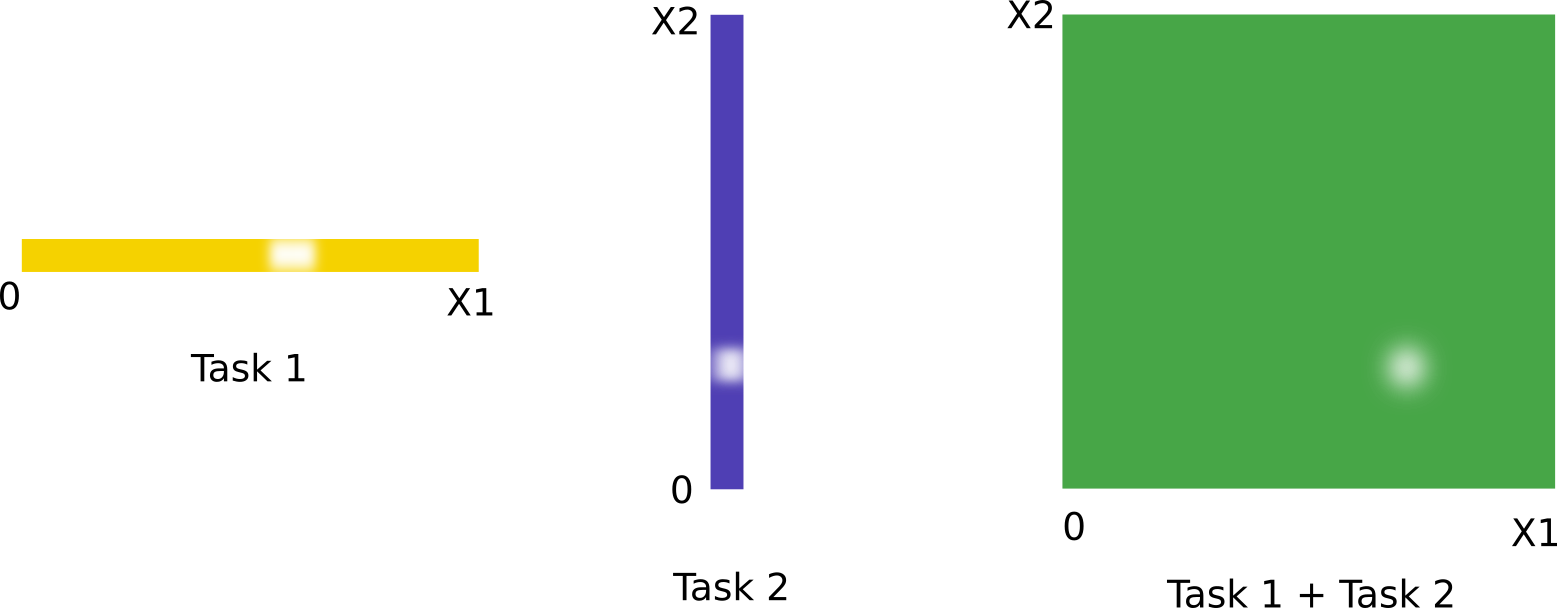
\includegraphics[scale=0.3]{img/understand1.png}
	\caption{Figure of reward-parameter map for general policy across tasks. $X_1, X_2$ are parameters for policy in Task 1 and Task 2 respectively. The color represent the reward value of parameterized policy with corresponding parameter values. The brighter it is, the larger the value is. And for a general policy across tasks with more parameters than a single task, there will always be a point for optimal policy across tasks.}
	\label{fig:understand1}
\end{figure}

\textbf{Reward-Parameter Map of the Meta-Initialization Policy (Second Type of Policy)}

For the meta-initialization policy, the neural network is supposed to contain the same numbers of parameters as a policy for single task, different from above general policy. Therefore there may not be an global optimal point across tasks but only some suboptimal points for each task, as shown in Fig. \ref{fig:understand2}.
\begin{figure}[htbp]
	\centering
	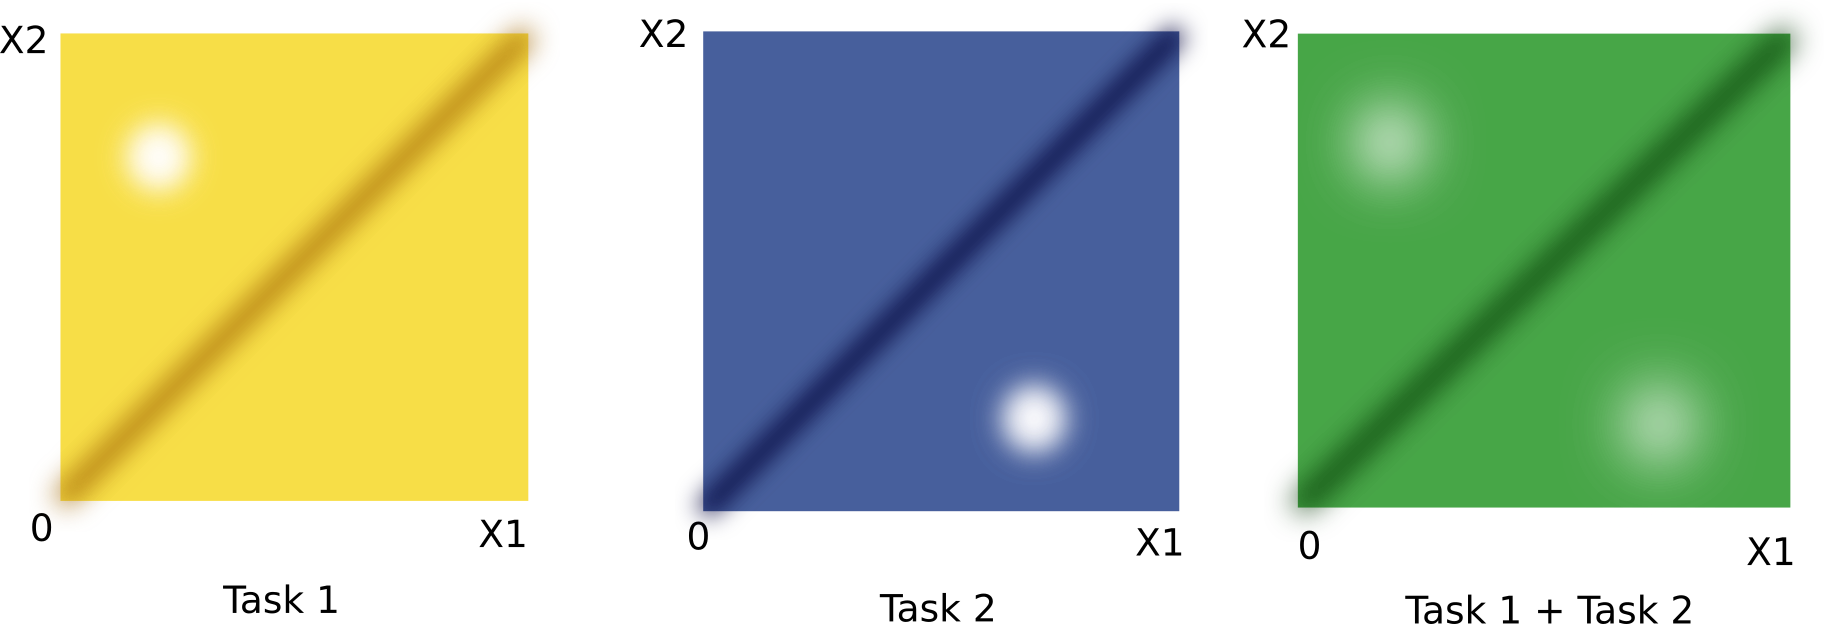
\includegraphics[scale=0.3]{img/understand2.png}
	\caption{Figure of reward-parameter map for meta-initialized policy across tasks. $X_1, X_2$ are parameters for single-task policy. The left and middle are reward maps for each of two tasks. And the right one is the reward map of the meta-initialization policy. The color represent the reward value of parameterized policy with corresponding parameter values. The brighter it is, the larger the value is. For meta-initialization policy, there may not be an global optimal point across tasks, but some suboptimal points for each task.}
	\label{fig:understand2}
\end{figure}

Fig. \ref{fig:understand3} shows how meta-learning makes the problem of learning across tasks easier with the meta-policy as initialization instead of a random initialization. We can also see that the meta-update could end up with a bad policy for every task but close to every optimal policy of each task in parameter space. \textbf{The meta-update in MAML actually tends to drift the initial policy to a point in parameter space where all optimal policies of each tasks in the task domain are isotropic for the meta-policy}.

\begin{figure}[htbp]
	\centering
	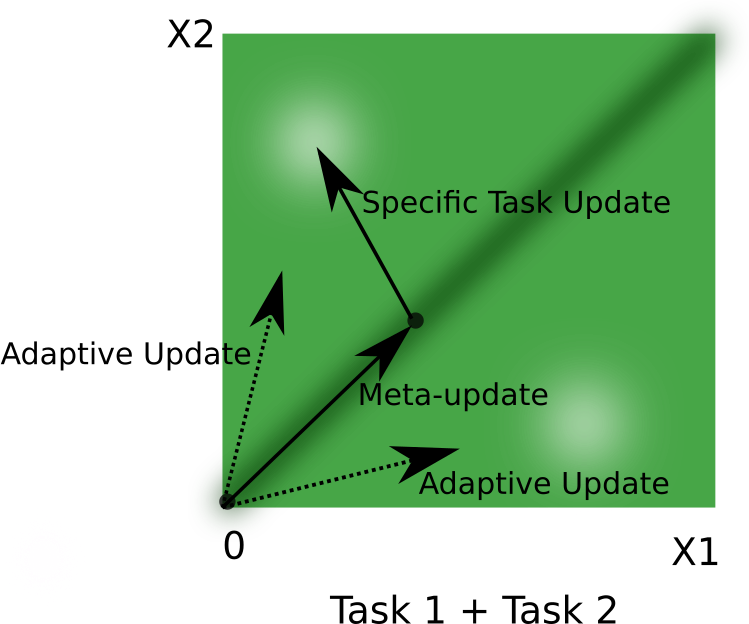
\includegraphics[scale=0.3]{img/understand3.png}
	\caption{Figure of reward-parameter map for meta-initialized policy across tasks using MAML with fixed-step stochastic gradient descent . $X_1, X_2$ are parameters for meta-initialized policy. The color represent the reward value of parameterized policy with corresponding parameter values. The brighter it is, the larger the value is. The dashed arrows shows the adaptive phase update for each task, and the solid arrow shows the possible meta-update. And the final solid arrow shows the update for a specific task after the initialization using the meta-policy. It shows how meta-learning makes the problem of learning across tasks easier with the meta-policy as initialization instead of a random initialization.}
	\label{fig:understand3}
\end{figure}

\subsubsection{A Potential Framework of Modified MAML}

Current MAML only keeps track of one step of adaptive updates, and update the initial policy parameter $\theta$ to be $\theta'_\mathcal{T}$. \textbf{The goal of MAML is to make the adaptively updated policy $\pi_{\theta'_\mathcal{T}}$ to have lower averaged loss value, instead of the initial policy $\pi_{\theta}$. Therefore, the resulting policy of this objective is a policy with a one-step update for a specific task to have lowest loss}. 

However, in practice, we do not expect the initialized policy to learn to be optimal policy with only one-step update, but $N$ steps. We can keep track of N-step adaptive updates and unroll the gradients for $N$th orders in the training phase for a more practical use. The resulting policy under this modified N-step MAML will be a policy with a N-step update for a specific task to have lowest loss.

Fig. \ref{fig:potential} shows a demo of computation graph for simple multiplication operations with a 4th order (4-step) MAML using Tensorflow.
\begin{figure}[htbp]
	\centering
	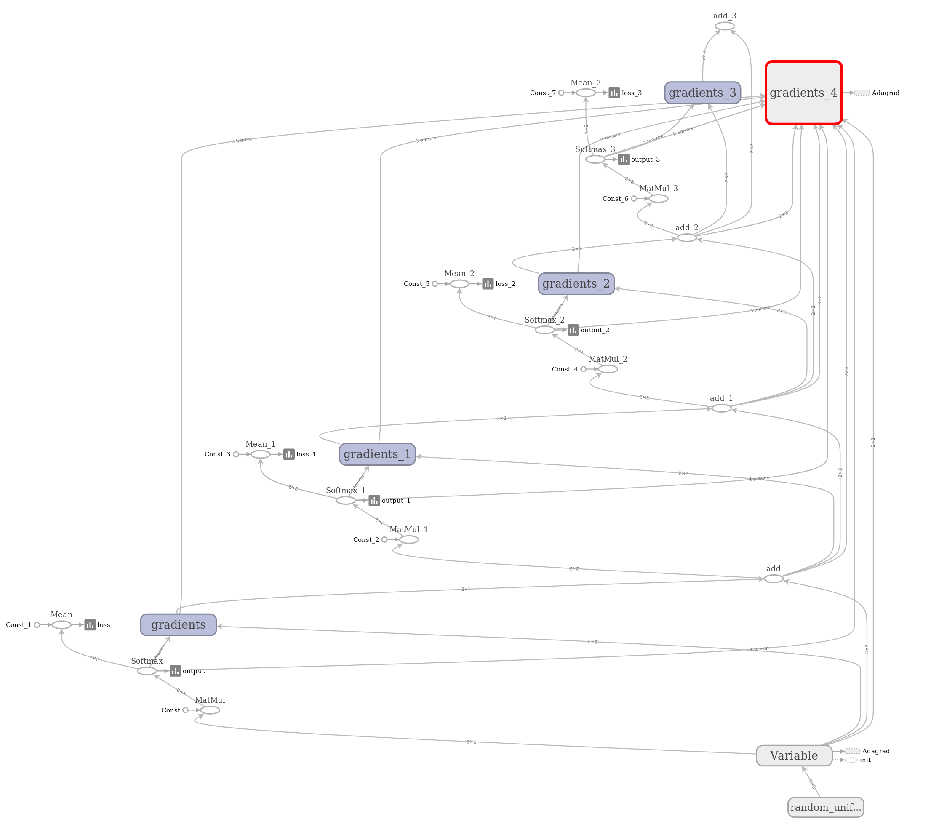
\includegraphics[scale=0.5]{img/potential.png}
	\caption{A demo computation graph of a 4th order MAML with Tensorflow.}
	\label{fig:potential}
\end{figure}

\subsubsection{Reptile + PPO}
The first order meta-learning method Reptile \cite{nichol2018first} can be applied in RL tasks as an initialization of the policy. The meta-RL methods can improve the learning efficiency of RL for a task domain without leveraging expert demonstrations. We experimentally first combine the Reptile method with PPO algorithm on a task domain of \textit{Reacher}, to compare the learning performances of meta-initialized PPO with PPO method from scratch.

\textbf{Experiment Settings:}

To alleviate computational burden for meta-training across tasks, we reduce the number of joints in \textit{Reacher} from 3 to 2. And the positions of the goal are randomly set in the 4th session of the screen as a task domain with different tasks of different goal positions. The range of the goal positions is shown in Fig. \ref{fig:meta_env}. 

\begin{figure}[htbp]
	\centering
	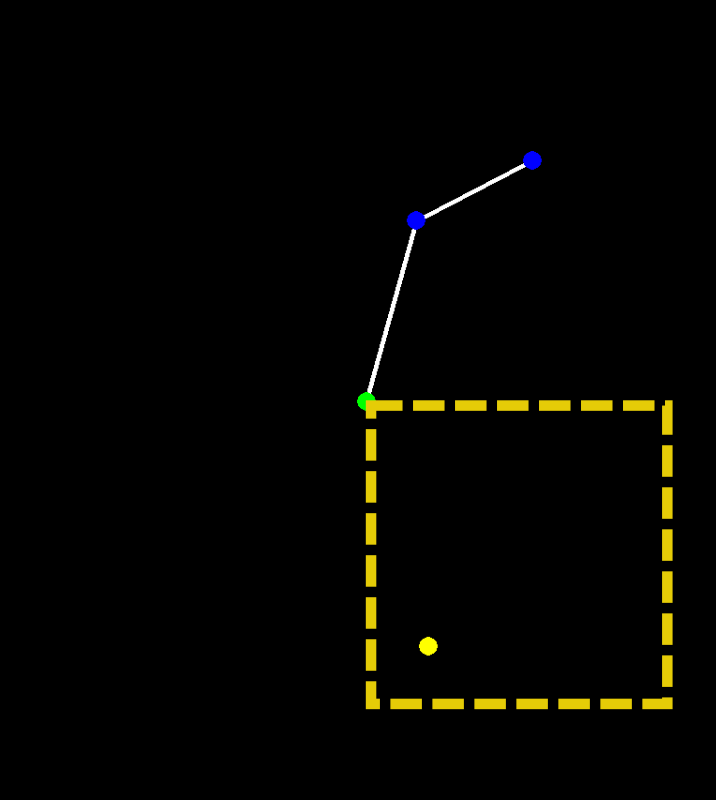
\includegraphics[scale=0.3]{img/meta_env.png}
	\caption{The two-joint \textit{Reacher} task domain with random goal positions in range of the yellow dashed square.}
	\label{fig:meta_env}
\end{figure}

The PPO algorithm contains an action policy and a value-evaluation policy which is also called the critic. There is only one hidden layer of size 100 for both the actor and the critic neural networks. The output activation function for the critic is the ReLu activation (keep positive), and for the actor are leakyReLu for the mean term and sigmoid for the variance term, as PPO is a nondeterministic policy with action values sampled from a normal distribution parameterized by the outputs of actor neural network. And we use a minimal value of $0.5$ for the variance term to boost explorations. The learning rates of the actor and the critic are $1\times10^{-4}, 2\times10^{-4}$ respectively. In practice, there are at least two approaches of implementing the PPO: (1). the clipping approach \cite{schulman2017proximal}; and (2). the KL-divergence penalty approach \cite{heess2017emergence}. We use the second one for experiment in this part.

The meta-learning process is set to have 10 random goals for 10 tasks in the regions we set, and each task is trained with a maximum of 1000 steps. And the meta-learned policy is used to initialize the policy for another task with a random goal position in range for test.

\textbf{Results:}

The comparison of learning performances of meta-initialized PPO with PPO method from scratch is shown in Fig. \ref{fig:reptile}. It clearly shows that the learning process with PPO initialized by meta-learned policy using Reptile have a better learning performances than PPO from scratch. Specifically, the starting point of the meta-initialized policy is much higher in reward than a random initialized policy, therefore ends up with a much faster learning process to achieve a higher averaged reward after the training process.

\begin{figure}[htbp]
	\centering
	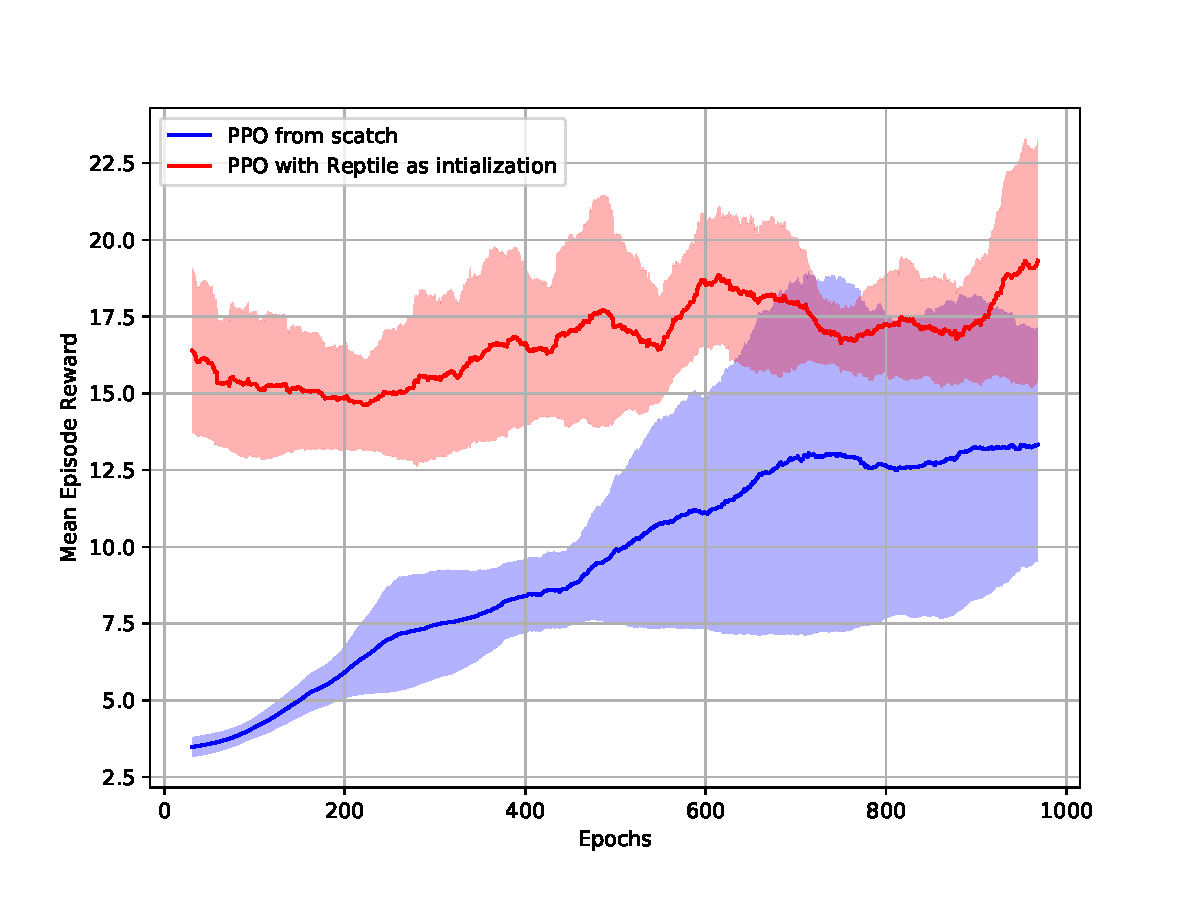
\includegraphics[scale=0.5]{img/Reptile.pdf}
	\caption{The comparison of learning performances of meta-initialized (Reptile) PPO with PPO from scratch on a two-joint \textit{Reacher} task.}
	\label{fig:reptile}
\end{figure}

\subsubsection{MAML + PPO}
We also applied MAML method for learning an initialization policy. The basic experiment settings are the same as the Reptile with PPO in the above section, and we use fisrt-order MAML (FOMAML) in practice. We use both two approaches for PPO implementation in this part.

Experiment results of PPO with FOMAML initialization and PPO from scratch are shown in Fig. \ref{fig:fomaml} with two versions of PPO. In both implementations, the MAML initialized PPO shows predominance over PPO from scratch for a random task in the domain.

\begin{figure}[htbp]
	\centering
	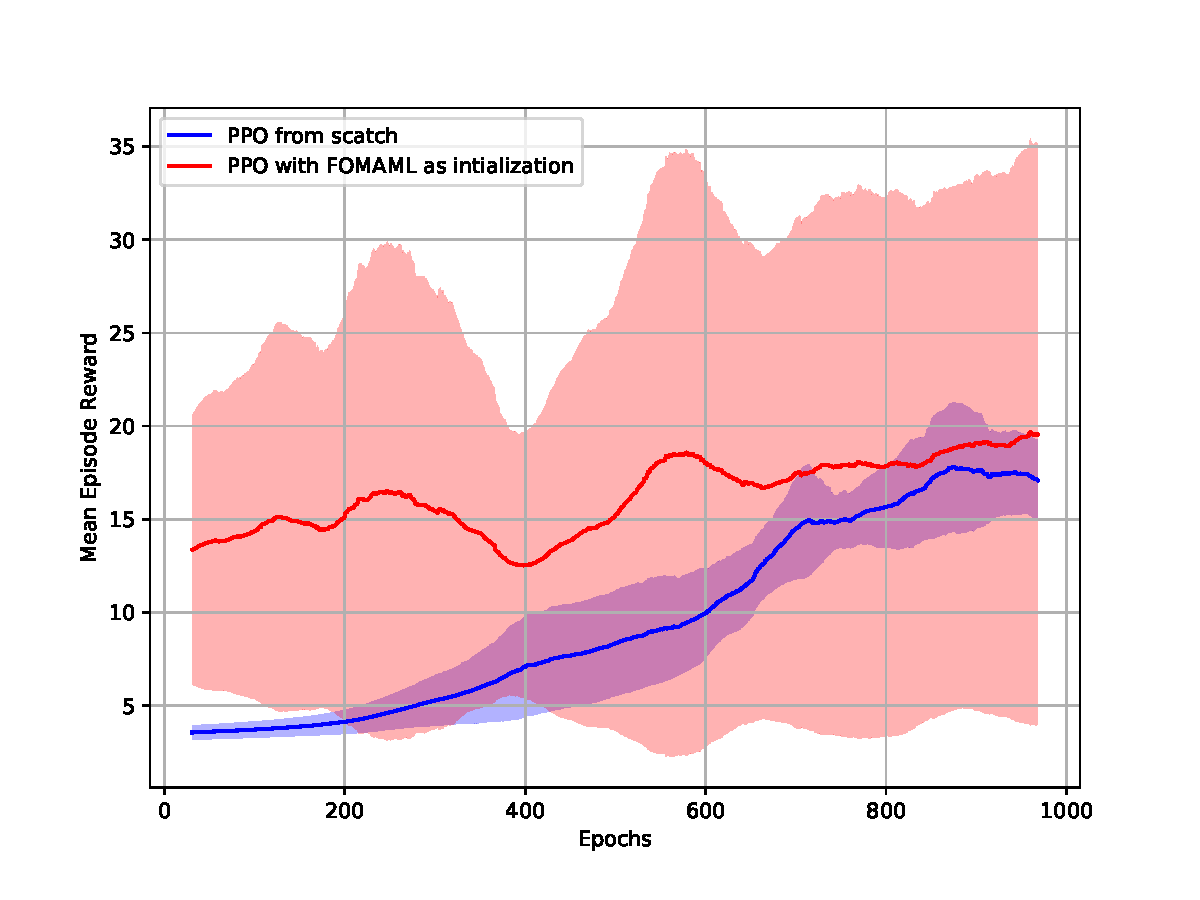
\includegraphics[scale=0.5]{img/fomaml.pdf}
	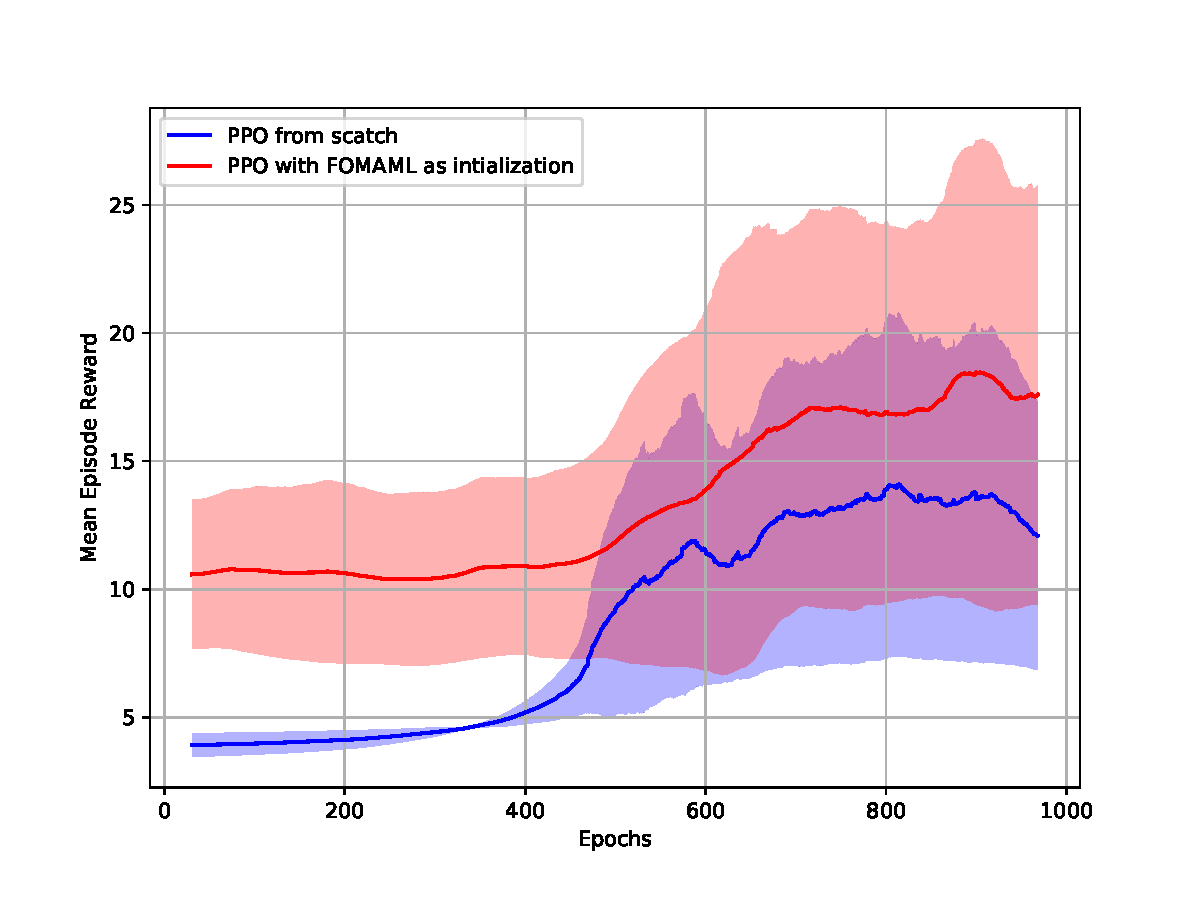
\includegraphics[scale=0.5]{img/fomaml2.pdf}
	\caption{The comparison of learning performances of meta-initialized (FOMAML) PPO with PPO from scratch on a two-joint \textit{Reacher} task. The top one is PPO with KL-divergence penalty, and the bottom one is PPO with clipping loss.}
	\label{fig:fomaml}
\end{figure}

\subsection{Universal Successor Representation for Efficient Reinforcement Learning}
Universal Successor Representation \cite{ma2018universal} provides a way to learn a universal value function approximator $V(s,g;\theta)$ for transfer learning across tasks in a task domain,where $s,g, \theta$ are state, goal and policy parameters respectively. It works for tasks with the same dynamics but different goals.

The reward function is factorized to be:
\begin{equation}
    r_g(s_t,a_t,s_{t+1})=\phi(s_t,a_t,s_{t+1})^T w_g
\end{equation}
where $\phi, w_g$ are features of state and goal-specific features of the reward. The value function can then be represented as:
\begin{equation}
\begin{aligned}
    V^\pi_g(s)&=\mathbb{E}^\pi[\sum_{t=0}^\infty r_g(s_t,a_t,s'_t)\gamma^t]\\
    &=\mathbb{E}^\pi[\sum_{t=0}^\infty \phi(s_t,a_t,s'_t)\gamma^t]^T w_g\\
    &=\Phi_g^\pi(s)^T w_g
\end{aligned}
\end{equation}
The Bellman equation for updating the value function is then transformed to the updating of the universal successor representations (USR) of state s:
\begin{equation}
    V_g^\pi=\mathbb{E}^\pi[r_g(s,a,s')+\gamma(s)V_g^\pi(s')],\quad \Phi_g^\pi(s)=\mathbb{E}^\pi[\phi(s,a,s')+\gamma(s)\Phi_g^\pi(s')]
\end{equation}
The $w_g$ is used as a mapping from the goal to corresponding goal-specific values, which can be parameterized by a neural network $w_g=w(g;\theta_w)$.

Through training across tasks with different goals, the learned universal value function approximator $V(s,g;\theta)$ is able to transfer quickly from general to a specific value function for the task. The method of USR is very similar to MuMoMAML \cite{vuorio2018toward} and methods in \cite{ammar2015autonomous} for knowledge transfer, all of which apply linear matrix multiplication and a trained mapping function to predict task-specific coefficients for fast adaptation to a task with new goal. The difference is only that they place the mapping on different function, i.e. on action policy for MuMoMAML, on the knowledge base for \cite{ammar2015autonomous} and on the value function with USR.

\newpage
\section{Conclusion}
\begin{table}
    \centering
\begin{tabular}{ |p{2.5cm}<{\centering}|p{3cm}<{\centering}|p{2cm}<{\centering}|p{3cm}<{\centering}|p{3cm}<{\centering}|}
\hline
Methods & Expert Demonstrations / Amounts & Pre-training & Improvement of Final Performances & Sensitivity to Hyperparameters\\
\hline
\hline
{Policy Replacement (DDPG)} & Needed / Large & Needed & 63\% (Distance) & Sensitive (Noise Scale, etc)\\
\hline 
{Residual Policy Learning (DDPG)} & Needed / Large  & Needed & 96\% (Distance) & Very Sensitive (Value Range, Noise Scale, etc)\\
\hline 
{DDPG from Demonstrations} & Needed / Small & Not Needed & 81\% (Distance) & Sensitive (Ratio of Demonstrations)\\
\hline
\hline 
Reptile + PPO & Not Needed & Needed & 46\% (Reward) & Not Sensitive\\
\hline 
FOMAML + PPO (KL-Penalty) & Not Needed & Needed & 18\% (Reward) & Not Sensitive\\
\hline
FOMAML + PPO (Cipping) & Not Needed & Needed & 35\% (Reward) & Not Sensitive\\
\hline 
\end{tabular}
\caption{Different methods for efficient reinforcement learning with or without demonstrations in experiments.}
\label{table:2}
\end{table}

In this paper, we investigate methods for improving the efficiency of reinforcement learning process in different approaches, including the approach of leveraging expert demonstrations and another approach of meta-learning across tasks without demonstrations. Experiments are conducted for both approaches, and a conclusive comparison of different methods in experiments is shown in Table \ref{table:2}. The contents of the table include: (1). whether the expert demonstrations are needed, and if so, the amount of demonstration data needed to guarantee a significant improvement; (2). whether pre-training a policy is needed in the methods before the RL process; (3). the improvement in the final performances of RL process with those methods, represented as a percentage, and the `Distance' and `Reward' indicates which measurement is used. The percentage denotes how much the increment is in final average reward ($R'/R_0-1$) if with `Reward', or how much the average final distance to the goal position is reduced ($1-D'/D_0$) if with `Distance'. And (4). whether the method is sensitive to hyperparameters in the tuning process of experiments. What kinds of hyperparameters could be of great effects are also shown in the brackets, if the method is sensitive to hyperparameters.

For the approach with expert demonstrations, the method with demonstrations directly fed into the memory buffer could lead to a robust improvement for reinforcement learning without fine-tuning, as long as the demonstrations are better in performances than general samples. And the method with residual policy learning could provide a much greater improvement in learning performances with a proper setting of the hyper-parameters (like output range, exploration noise scale, etc) and a good initialization policy. The disadvantages of this approach includes the difficulties in generating demonstration data, especially in real-world applications, and the instability of applying an initialization policy pre-trained with small amounts of data. 

For another approach of meta-learning across tasks without leveraging demonstrations, methods like first-order modal-agnostic meta-learning and Reptile both accelerate the reinforcement learning process significantly when applied as an initialization policy. However, methods based on meta-learning suffers from the difficulties in training a meta-policy and the cost of the pre-training, including the time consumption and the large number of samples required in the process. 

Those methods in both approaches provide heuristic ideas about how to improve the efficiency of reinforcement learning, which could be a critical problem for learning in a human way. And it could be of significance when applied in real-world applications like robotic control.  


\newpage
\medskip
 
\bibliographystyle{unsrt}
\bibliography{ref}

\end{document}
